\documentclass[11pt,a4paper]{scrartcl}
\usepackage{gram}
\usetikzlibrary{arrows}
\usetikzlibrary{patterns}
\usepackage{svg}
\usepackage{pgfplots}
\pgfplotsset{compat=1.15}
\usetikzlibrary{arrows}
\pagecolor{fizikawhite}
\usepackage{gensymb}
\usepackage{enumitem}
\usepackage{wrapfig}






\title{FIZIKA Round-2}
\author{GRAMOLY}
\date{September 2021}

\begin{document}
\begin{tcolorbox}

The scoring criteria is as follows:
There are no negatives for integer valued problems:

In case of Multiple choice problems, partials will be awarded as follows
Marking Scheme:
Full marks, $+4$ if all the correct options are marked.
Partial marks , $+1$ for each correct option provided NO incorrect option is marked.
Zero marks, if no option is marked.
Negative marks, $-1$

The raw score of the problem is scaled based on its difficulty as follows:
In case of integer valued problems:
$$Marks = max(8.5-ln(N), 4)$$
Where N is the number of people who got the question correct

\textbf{In case of Multiple choice questions:}
$$Marks = max\left(\left(\frac{8.5\cdot A}{4}-ln(N)\right), A\right)$$
Where N is the number of people who got the question correct
A is the the aggregate marks the person has scored in the question after taking partials into account.

${\textbf{Selection criteria for round 2:}}$

After every participant has been scored the following criteria will be used for selection:

$$\textbf{Final Marks}=\frac{\text{Your marks in round $1$}}{\text{Average Marks scored in round $1$}}\cdot 10 + \frac{\text{Your marks in round $2$}}{\text{Average Marks scored in round $2$}}\cdot 90$$

The top 50 from the final mark list will be selected for round 3.
\end{tcolorbox}

\pagebreak
\vspace{10mm}
\vspace{10mm}%\section{Problem 1}

\begin{problem}

A solid paraboloid of base radius $R_0$ and height $h_0$ is having uniform volume mass density $\rho_s$ is inverted and placed just above the surface as shown, of a liquid having volume mass density $\rho_L$. When paraboloid is released from rest it has been observed that when it becomes completely submerged in the liquid the paraboloid comes to rest again. What is the ratio of $\frac{\rho_L}{\rho_s}$ for such a paraboloid. There exist a uniform gravity of $g$. Assume that the liquid body is very large so that liquid level is not changing as the paraboloid enters into liquid.\\\



\begin{center}
    

\tikzset{every picture/.style={line width=0.75pt}} %set default line width to 0.75pt        

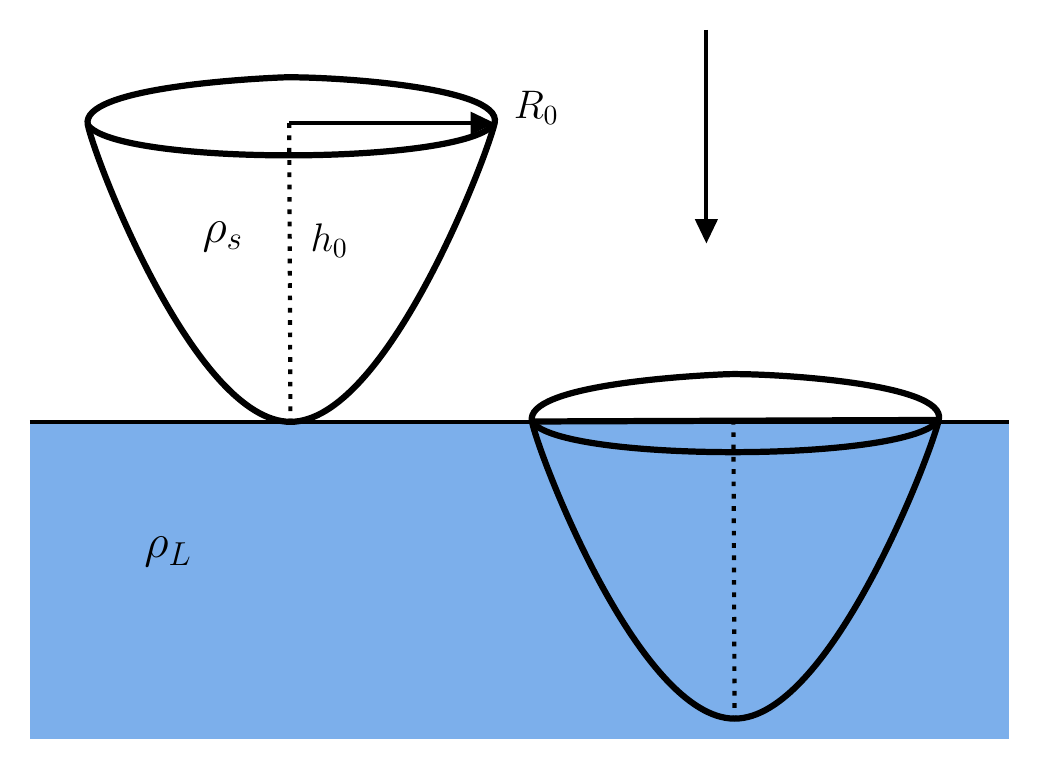
\begin{tikzpicture}[x=0.75pt,y=0.75pt,yscale=-1,xscale=1]
%uncomment if require: \path (0,484); %set diagram left start at 0, and has height of 484

%Shape: Rectangle [id:dp3471801487731352] 
\draw  [draw opacity=0][fill={rgb, 255:red, 124; green, 175; blue, 235 }  ,fill opacity=1 ] (98,262) -- (570,262) -- (570,415) -- (98,415) -- cycle ;
%Straight Lines [id:da5548236311335806] 
\draw [line width=1.5]    (98,262) -- (570,262) ;

%Shape: Polygon Curved [id:ds773303895242313] 
\draw  [line width=2.25]  (433.2,239.08) .. controls (450.08,238.34) and (540.39,242.75) .. (535.98,261.1) .. controls (531.58,279.46) and (483.12,405) .. (437.6,405) .. controls (392.08,405) and (343.63,279.46) .. (339.96,261.84) .. controls (336.28,244.21) and (416.31,239.81) .. (433.2,239.08) -- cycle ;
%Curve Lines [id:da31733221468341055] 
\draw [line width=2.25]    (339.96,261.84) .. controls (353.17,281.66) and (522.77,281.66) .. (535.98,261.1) ;
%Straight Lines [id:da21592815385663977] 
\draw [line width=2.25]    (339.96,261.84) -- (535.98,261.1) ;

%Shape: Polygon Curved [id:ds08432726498677523] 
\draw  [line width=2.25]  (219.2,96.08) .. controls (236.08,95.34) and (326.39,99.75) .. (321.98,118.1) .. controls (317.58,136.46) and (269.12,262) .. (223.6,262) .. controls (178.08,262) and (129.63,136.46) .. (125.96,118.84) .. controls (122.28,101.21) and (202.31,96.81) .. (219.2,96.08) -- cycle ;
%Curve Lines [id:da7771060739273872] 
\draw [line width=2.25]    (125.96,118.84) .. controls (139.17,138.66) and (308.77,138.66) .. (321.98,118.1) ;
%Straight Lines [id:da7259197731975575] 
\draw [line width=1.5]    (223,118.1) -- (317.98,118.1) ;
\draw [shift={(321.98,118.1)}, rotate = 180] [fill={rgb, 255:red, 0; green, 0; blue, 0 }  ][line width=0.08]  [draw opacity=0] (11.61,-5.58) -- (0,0) -- (11.61,5.58) -- cycle    ;
%Straight Lines [id:da8770684220899543] 
\draw [line width=1.5]  [dash pattern={on 1.69pt off 2.76pt}]  (223,118.1) -- (223.6,262) ;
%Straight Lines [id:da8910781285402045] 
\draw [line width=1.5]  [dash pattern={on 1.69pt off 2.76pt}]  (437,261.1) -- (437.6,405) ;
%Straight Lines [id:da08400828585401765] 
\draw [line width=1.5]    (424,73.1) -- (424,172) ;
\draw [shift={(424,176)}, rotate = 270] [fill={rgb, 255:red, 0; green, 0; blue, 0 }  ][line width=0.08]  [draw opacity=0] (11.61,-5.58) -- (0,0) -- (11.61,5.58) -- cycle    ;

% Text Node
\draw (180,164.4) node [anchor=north west][inner sep=0.75pt]  [font=\LARGE]  {$\rho _{s}$};
% Text Node
\draw (232,165.4) node [anchor=north west][inner sep=0.75pt]  [font=\Large]  {$h_{0}$};
% Text Node
\draw (152,316.4) node [anchor=north west][inner sep=0.75pt]  [font=\LARGE]  {$\rho _{L}$};
% Text Node
\draw (330,101.4) node [anchor=north west][inner sep=0.75pt]  [font=\Large]  {$R_{0}$};


\end{tikzpicture}

\end{center}

\end{problem}
\begin{flushright}
\textbf{\Large{-Proposed by Nitin Sachan}}
\end{flushright}
\begin{solution}
{\Large{\textbf{Answer: 3}}}\\
Net Force on the paraboloid:\newline
$mg-\rho_{L} \cdot \frac{1}{2} \pi x^2y \cdot g = m \cdot \frac{dv}{dt}$\newline
$v \cdot \frac{dv}{dy} = \frac{dv}{dt} = g- \frac{\rho_{L}}{\rho_{S}} \cdot \frac{x^2}{R^2} \cdot \frac{yg}{H}\
\implies g - \frac{\rho_L}{\rho_S} \cdot \frac{yR^2}{H \cdot R^2} \cdot {yg}{H}$
\begin{center}
    \tikzset{every picture/.style={line width=0.75pt}} %set default line width to 0.75pt        

\begin{tikzpicture}[x=0.75pt,y=0.75pt,yscale=-1,xscale=1]
%uncomment if require: \path (0,300); %set diagram left start at 0, and has height of 300

%Straight Lines [id:da16192514966136584] 
\draw  [dash pattern={on 4.5pt off 4.5pt}]  (259.3,42.15) -- (259.3,231.15) ;
\draw [shift={(259.3,40.15)}, rotate = 90] [color={rgb, 255:red, 0; green, 0; blue, 0 }  ][line width=0.75]    (10.93,-3.29) .. controls (6.95,-1.4) and (3.31,-0.3) .. (0,0) .. controls (3.31,0.3) and (6.95,1.4) .. (10.93,3.29)   ;
%Shape: Parabola [id:dp4832957054331293] 
\draw   (177,61.15) .. controls (232.77,280.95) and (288.53,280.95) .. (344.3,61.15) ;
%Straight Lines [id:da5837249741600998] 
\draw  [dash pattern={on 4.5pt off 4.5pt}]  (260.65,226) -- (443.3,225.16) ;
\draw [shift={(445.3,225.15)}, rotate = 539.73] [color={rgb, 255:red, 0; green, 0; blue, 0 }  ][line width=0.75]    (10.93,-3.29) .. controls (6.95,-1.4) and (3.31,-0.3) .. (0,0) .. controls (3.31,0.3) and (6.95,1.4) .. (10.93,3.29)   ;
%Straight Lines [id:da5738196907513968] 
\draw    (360.3,159.18) -- (362.24,224.18) ;
\draw [shift={(362.3,226.18)}, rotate = 268.29] [color={rgb, 255:red, 0; green, 0; blue, 0 }  ][line width=0.75]    (10.93,-3.29) .. controls (6.95,-1.4) and (3.31,-0.3) .. (0,0) .. controls (3.31,0.3) and (6.95,1.4) .. (10.93,3.29)   ;
%Straight Lines [id:da587282662068833] 
\draw    (360.3,126.18) -- (360.3,63.15) ;
\draw [shift={(360.3,61.15)}, rotate = 450] [color={rgb, 255:red, 0; green, 0; blue, 0 }  ][line width=0.75]    (10.93,-3.29) .. controls (6.95,-1.4) and (3.31,-0.3) .. (0,0) .. controls (3.31,0.3) and (6.95,1.4) .. (10.93,3.29)   ;
%Straight Lines [id:da3361261661699195] 
\draw    (262.3,61.18) -- (342.3,61.15) ;
\draw [shift={(344.3,61.15)}, rotate = 539.97] [fill={rgb, 255:red, 0; green, 0; blue, 0 }  ][line width=0.08]  [draw opacity=0] (12,-3) -- (0,0) -- (12,3) -- cycle    ;
\draw [shift={(260.3,61.18)}, rotate = 359.97] [fill={rgb, 255:red, 0; green, 0; blue, 0 }  ][line width=0.08]  [draw opacity=0] (12,-3) -- (0,0) -- (12,3) -- cycle    ;

% Text Node
\draw (353,133.4) node [anchor=north west][inner sep=0.75pt]  [font=\small]  {$H$};
% Text Node
\draw (294,43.4) node [anchor=north west][inner sep=0.75pt]    {$R$};
% Text Node
\draw (254,10.4) node [anchor=north west][inner sep=0.75pt]    {$y$};
% Text Node
\draw (450,218.4) node [anchor=north west][inner sep=0.75pt]    {$x$};


\end{tikzpicture}
\end{center}

$v\cdot \frac{dv}{dy} = g - \frac{g\cdot \rho_{L}}{H^2 \rho_{S}} \cdot y^2 $ \newline
Integrating this using $v_{i}=v{f}=0$ and putting appropriate limits we get:\newline
$\int_{0}^0 v\cdot dv = g\cdot \int_{0}^H {dy}- \frac{g \rho_{L}}{H^2 \rho_{S}} \cdot \int_{0}^H {y^2 dy}$\newline
\begin{center}
    \tikzset{every picture/.style={line width=0.75pt}} %set default line width to 0.75pt        

\begin{tikzpicture}[x=0.75pt,y=0.75pt,yscale=-1,xscale=1]
%uncomment if require: \path (0,300); %set diagram left start at 0, and has height of 300

%Shape: Parabola [id:dp1391967798733198] 
\draw   (192,27.15) .. controls (247.77,246.95) and (303.53,246.95) .. (359.3,27.15) ;
%Straight Lines [id:da09572954967849823] 
\draw    (337.3,101.44) -- (520.3,102.44) ;
%Straight Lines [id:da9217126763484371] 
\draw    (29.3,96.44) -- (212.3,97.44) ;
%Straight Lines [id:da6577982772501108] 
\draw  [dash pattern={on 4.5pt off 4.5pt}]  (212.3,97.44) -- (337.3,101.44) ;
%Straight Lines [id:da7289890606289933] 
\draw    (274.3,90.44) -- (275.27,31.43) ;
\draw [shift={(275.3,29.44)}, rotate = 450.94] [color={rgb, 255:red, 0; green, 0; blue, 0 }  ][line width=0.75]    (10.93,-3.29) .. controls (6.95,-1.4) and (3.31,-0.3) .. (0,0) .. controls (3.31,0.3) and (6.95,1.4) .. (10.93,3.29)   ;
%Straight Lines [id:da9640695780885002] 
\draw    (274.8,99.44) -- (335.3,101.37) ;
\draw [shift={(337.3,101.44)}, rotate = 181.83] [color={rgb, 255:red, 0; green, 0; blue, 0 }  ][line width=0.75]    (10.93,-3.29) .. controls (6.95,-1.4) and (3.31,-0.3) .. (0,0) .. controls (3.31,0.3) and (6.95,1.4) .. (10.93,3.29)   ;
%Straight Lines [id:da5796457891223594] 
\draw    (279.3,166.44) -- (276.39,232.44) ;
\draw [shift={(276.3,234.44)}, rotate = 272.53] [color={rgb, 255:red, 0; green, 0; blue, 0 }  ][line width=0.75]    (10.93,-3.29) .. controls (6.95,-1.4) and (3.31,-0.3) .. (0,0) .. controls (3.31,0.3) and (6.95,1.4) .. (10.93,3.29)   ;
%Straight Lines [id:da20985358944343258] 
\draw    (344.27,109.43) -- (343.33,166.44) ;
\draw [shift={(343.3,168.44)}, rotate = 270.94] [color={rgb, 255:red, 0; green, 0; blue, 0 }  ][line width=0.75]    (10.93,-4.9) .. controls (6.95,-2.3) and (3.31,-0.67) .. (0,0) .. controls (3.31,0.67) and (6.95,2.3) .. (10.93,4.9)   ;
\draw [shift={(344.3,107.44)}, rotate = 90.94] [color={rgb, 255:red, 0; green, 0; blue, 0 }  ][line width=0.75]    (10.93,-4.9) .. controls (6.95,-2.3) and (3.31,-0.67) .. (0,0) .. controls (3.31,0.67) and (6.95,2.3) .. (10.93,4.9)   ;
%Straight Lines [id:da7879694703315596] 
\draw  [dash pattern={on 4.5pt off 4.5pt}]  (195.3,139.44) -- (194.32,226.44) ;
\draw [shift={(194.3,228.44)}, rotate = 270.64] [color={rgb, 255:red, 0; green, 0; blue, 0 }  ][line width=0.75]    (10.93,-3.29) .. controls (6.95,-1.4) and (3.31,-0.3) .. (0,0) .. controls (3.31,0.3) and (6.95,1.4) .. (10.93,3.29)   ;

% Text Node
\draw (189,230.4) node [anchor=north west][inner sep=0.75pt]    {$a$};
% Text Node
\draw (262,2.4) node [anchor=north west][inner sep=0.75pt]    {$F_{u}{}_{p}$};
% Text Node
\draw (264,237.4) node [anchor=north west][inner sep=0.75pt]    {$mg$};
% Text Node
\draw (349,125.4) node [anchor=north west][inner sep=0.75pt]    {$y$};
% Text Node
\draw (302,78.4) node [anchor=north west][inner sep=0.75pt]    {$x$};


\end{tikzpicture}
\end{center}
$0 = gH - \frac{g}{3}\frac{\rho_L}{\rho_S} \cdot H$\newline
Hence,
$\boxed{ \frac{\rho_L}{\rho_S} = 3}$\\

Also an energy conservation approach can be applied to shorten the solution.
\end{solution}


\vspace{10mm}%\section{Problem 2}

\begin{problem}

You have a spectrometer of spectral resolving power $5\cdot 10^4$. Say $n_1$ is the maximum value of principal quantum number for which the resulting energy spectra can be distinguished clearly from its neighbours. Also $n_0$ denotes the minimum value of principal quantum number for which a human eye can see the atomic transition. Find the value of $\boxed{n_1-n_{0}}$. We are only working in the Balmer transitions of hydrogen atom.

Value of Rydberg constant is $R=1\cdot 10^7$ and maximum wavelength eye can see is $700 nm$
\end{problem}
\begin{flushright}
\textbf{\Large{Proposed by Abhiram Cherukupalli}}
\end{flushright}
\begin{solution}
{\Large{\textbf{Answer: 69 }}}\\

\begin{equation*}
    \boxed{\frac{1}{\lambda}=R(\frac{1}{4}-\frac{1}{n^2}),\  n \geq 3}
    \label{eq:1}
\end{equation*}
$$\frac{\Delta \lambda}{\Delta n}\approx \frac{d \lambda}{d n} $$
Note that though this is an approximate method, it can be verified by desmos, and the answers are close.

Now using this logic we can differentiate \eqref{eq:1} to get:

$$\frac{d \lambda}{d n} =-\frac{2R}{n^3} {\lambda}^2 \approx \frac{\Delta \lambda}{\Delta n}$$



The beautiful step here is to take $\Delta n = 1$, as it has to be distinguished from its neighbours.

This gives us: $$\frac{\Delta \lambda}{ \lambda} \approx \frac{2R}{{n_1}^3}\lambda $$

The spectral power $$\frac{\lambda}{\Delta \lambda}=\frac{{n_1}^3}{2}(\frac{1}{4}-\frac{1}{n^2})<5\cdot 10^4$$

$$\implies n_1 < 73.69 \implies \boxed{n_1=73}$$

Calculation of $n_0$ is straight-forward:-

\begin{equation*}
    n_0=\sqrt{\frac{4R\lambda}{R\lambda - 4}}=3.055
\end{equation*}

Hence $n_0=4$ and $\boxed{n_1-n_0=69}$

Note that we have to use the value of R mentioned in the question not the exact value also note that though the human eye data is close the value is very easy to calculate by hand as we get $\frac{4R\lambda}{R\lambda - 4} > 9$ without need of much calculation as $R\lambda=7$.






\end{solution}
\vspace{10mm}%\section{Problem 3}
\begin{problem}

We have a loop of radii 80 cm with 2 identical beads of mass 9 kg and radius 6.97 cm inserted in it, free to move without friction. The loop starts rotating along the diameter with an angular velocity $\omega=5$ rad/s. If the angle lower bead makes $\theta_1$ and upper bead makes $\theta_2$ then report $\boxed{\frac{\theta_1 + 3\theta_2}{50}}$. You may assume that both beads are displaced to the same side of loop. \\

Use $\arcsin\left(\frac{6.97}{80}\right) \approx  5\degree$,$\cos 5\degree \approx 0.9962$, $\cos 10 \degree \approx 0.9848$, $\arccos(0.5058) \approx 60 \degree $ and $\arccos(0.2529) \approx 75\degree$


\begin{center}
    

\tikzset{every picture/.style={line width=0.75pt}} %set default line width to 0.75pt        

\begin{tikzpicture}[x=0.75pt,y=0.75pt,yscale=-1,xscale=1]
%uncomment if require: \path (0,300); %set diagram left start at 0, and has height of 300

%Shape: Circle [id:dp06516168851386683] 
\draw   (235,146) .. controls (235,95.19) and (276.19,54) .. (327,54) .. controls (377.81,54) and (419,95.19) .. (419,146) .. controls (419,196.81) and (377.81,238) .. (327,238) .. controls (276.19,238) and (235,196.81) .. (235,146) -- cycle ;
%Straight Lines [id:da1653687189992059] 
\draw  [dash pattern={on 4.5pt off 4.5pt}]  (327,14) -- (327,279) ;
%Curve Lines [id:da2810346087828328] 
\draw    (309,28) .. controls (325.46,40.61) and (338.26,32.75) .. (344.13,28.49) ;
\draw [shift={(346.5,26.75)}, rotate = 505.49] [fill={rgb, 255:red, 0; green, 0; blue, 0 }  ][line width=0.08]  [draw opacity=0] (8.93,-4.29) -- (0,0) -- (8.93,4.29) -- cycle    ;
%Straight Lines [id:da15311693951538174] 
\draw    (327,146) -- (410.26,169.22) ;
\draw [shift={(415.75,170.75)}, rotate = 15.58] [color={rgb, 255:red, 0; green, 0; blue, 0 }  ][line width=0.75]      (0, 0) circle [x radius= 6.7, y radius= 6.7]   ;
%Straight Lines [id:da023184186627863035] 
\draw    (327,146.5) -- (405.8,181.68) ;
\draw [shift={(411,184)}, rotate = 24.06] [color={rgb, 255:red, 0; green, 0; blue, 0 }  ][line width=0.75]      (0, 0) circle [x radius= 6.7, y radius= 6.7]   ;
%Shape: Arc [id:dp8288399209455772] 
\draw  [draw opacity=0] (339.33,149.66) .. controls (337.11,154.07) and (333,157.41) .. (327.88,158.42) -- (324.63,141.97) -- cycle ; \draw   (339.33,149.66) .. controls (337.11,154.07) and (333,157.41) .. (327.88,158.42) ;
%Shape: Arc [id:dp39428024939745066] 
\draw  [draw opacity=0] (368.41,157.53) .. controls (365.15,171.03) and (354.3,181.92) .. (339.95,184.33) .. controls (335.38,185.1) and (330.87,184.94) .. (326.61,183.99) -- (333.98,148.81) -- cycle ; \draw   (368.41,157.53) .. controls (365.15,171.03) and (354.3,181.92) .. (339.95,184.33) .. controls (335.38,185.1) and (330.87,184.94) .. (326.61,183.99) ;
%Straight Lines [id:da6712551954498671] 
\draw    (459.33,83) -- (459.33,162.67) ;
\draw [shift={(459.33,165.67)}, rotate = 270] [fill={rgb, 255:red, 0; green, 0; blue, 0 }  ][line width=0.08]  [draw opacity=0] (8.93,-4.29) -- (0,0) -- (8.93,4.29) -- cycle    ;

% Text Node
\draw (349.83,19.9) node [anchor=north west][inner sep=0.75pt]    {$\omega $};
% Text Node
\draw (347.5,188.15) node [anchor=north west][inner sep=0.75pt]    {$\theta _{1}$};
% Text Node
\draw (332,157.65) node [anchor=north west][inner sep=0.75pt]    {$\theta _{2}$};
% Text Node
\draw (466.5,130.73) node [anchor=north west][inner sep=0.75pt]    {$g$};


\end{tikzpicture}

\end{center}







\end{problem}
\begin{flushright}
\textbf{\Large{-Proposed by Atharva Mahajan}}
\end{flushright}

\begin{solution}
{\Large{\textbf{Answer: 5}}}\\


\begin{center}
    

\tikzset{every picture/.style={line width=0.75pt}} %set default line width to 0.75pt        
\begin{tikzpicture}[x=0.75pt,y=0.75pt,yscale=-1,xscale=1]
%uncomment if require: \path (0,300); %set diagram left start at 0, and has height of 300

%Shape: Circle [id:dp24911765787641071] 
\draw   (225,145.15) .. controls (225,85.97) and (272.97,38) .. (332.15,38) .. controls (391.33,38) and (439.3,85.97) .. (439.3,145.15) .. controls (439.3,204.33) and (391.33,252.3) .. (332.15,252.3) .. controls (272.97,252.3) and (225,204.33) .. (225,145.15) -- cycle ;
%Straight Lines [id:da5018260597696493] 
\draw    (327.3,3.33) -- (331.3,289.33) ;
%Straight Lines [id:da6108274607173252] 
\draw    (329.3,146.33) -- (434,182.78) ;
%Straight Lines [id:da39106850530739945] 
\draw    (329.3,146.33) -- (438.3,165.63) ;
%Curve Lines [id:da07930156857159676] 
\draw    (329.3,159.78) .. controls (335.3,162.78) and (341.3,158.74) .. (344.3,151.78) ;
%Curve Lines [id:da8784000551384208] 
\draw    (330,176.26) .. controls (338.3,183.78) and (363.3,165.15) .. (361.3,152.15) ;
%Curve Lines [id:da7223231648834563] 
\draw    (307.3,13.85) .. controls (317.97,33) and (335.22,31.55) .. (349.94,17.22) ;
\draw [shift={(351.3,15.85)}, rotate = 493.89] [color={rgb, 255:red, 0; green, 0; blue, 0 }  ][line width=0.75]    (10.93,-3.29) .. controls (6.95,-1.4) and (3.31,-0.3) .. (0,0) .. controls (3.31,0.3) and (6.95,1.4) .. (10.93,3.29)   ;
%Shape: Circle [id:dp671132518442334] 
\draw   (426.13,181.75) .. controls (426.13,176.83) and (430.11,172.85) .. (435.03,172.85) .. controls (439.94,172.85) and (443.93,176.83) .. (443.93,181.75) .. controls (443.93,186.66) and (439.94,190.65) .. (435.03,190.65) .. controls (430.11,190.65) and (426.13,186.66) .. (426.13,181.75) -- cycle ;
%Shape: Circle [id:dp8612535744420371] 
\draw   (430.48,164.83) .. controls (430.67,160.25) and (434.54,156.68) .. (439.13,156.87) .. controls (443.72,157.06) and (447.28,160.94) .. (447.09,165.53) .. controls (446.9,170.11) and (443.03,173.68) .. (438.44,173.49) .. controls (433.85,173.3) and (430.28,169.42) .. (430.48,164.83) -- cycle ;
%Curve Lines [id:da2957584498070891] 
\draw    (390.3,162.11) .. controls (432.87,144.29) and (447.02,131.37) .. (453.12,85.51) ;
\draw [shift={(453.3,84.11)}, rotate = 457.28] [color={rgb, 255:red, 0; green, 0; blue, 0 }  ][line width=0.75]    (10.93,-4.9) .. controls (6.95,-2.3) and (3.31,-0.67) .. (0,0) .. controls (3.31,0.67) and (6.95,2.3) .. (10.93,4.9)   ;

% Text Node
\draw (335.2,154.73) node [anchor=north west][inner sep=0.75pt]  [font=\scriptsize,rotate=-359.82,xslant=0.03]  {$ \begin{array}{l}
\theta _{1}\\
\end{array}$};
% Text Node
\draw (354.3,165.21) node [anchor=north west][inner sep=0.75pt]  [font=\scriptsize]  {$\theta _{2}$};
% Text Node
\draw (451,154.4) node [anchor=north west][inner sep=0.75pt]  [font=\footnotesize]  {$2$};
% Text Node
\draw (445.93,185.15) node [anchor=north west][inner sep=0.75pt]  [font=\footnotesize]  {$7$};
% Text Node
\draw (433,43.4) node [anchor=north west][inner sep=0.75pt]  [font=\footnotesize]  {$R\ sin\Bigl(\frac{\theta _{2} -\theta _{1}}{2}\Bigr) =r\ $};
\end{tikzpicture}
\end{center}






\begin{center}
\tikzset{every picture/.style={line width=0.75pt}} %set default line width to 0.75pt        

\begin{tikzpicture}[x=0.75pt,y=0.75pt,yscale=-1,xscale=1]
%uncomment if require: \path (0,224); %set diagram left start at 0, and has height of 224

%Shape: Circle [id:dp9602804073456632] 
\draw   (228,129.5) .. controls (228,109.34) and (244.34,93) .. (264.5,93) .. controls (284.66,93) and (301,109.34) .. (301,129.5) .. controls (301,149.66) and (284.66,166) .. (264.5,166) .. controls (244.34,166) and (228,149.66) .. (228,129.5) -- cycle ;
%Shape: Circle [id:dp6257962402775974] 
\draw   (278,75.5) .. controls (278,55.34) and (294.34,39) .. (314.5,39) .. controls (334.66,39) and (351,55.34) .. (351,75.5) .. controls (351,95.66) and (334.66,112) .. (314.5,112) .. controls (294.34,112) and (278,95.66) .. (278,75.5) -- cycle ;
%Straight Lines [id:da7301828267626138] 
\draw    (264.5,129.5) -- (265.96,205.69) ;
\draw [shift={(266,207.69)}, rotate = 268.9] [color={rgb, 255:red, 0; green, 0; blue, 0 }  ][line width=0.75]    (10.93,-3.29) .. controls (6.95,-1.4) and (3.31,-0.3) .. (0,0) .. controls (3.31,0.3) and (6.95,1.4) .. (10.93,3.29)   ;
%Straight Lines [id:da4765928608165044] 
\draw    (314.5,75.5) -- (315.96,151.69) ;
\draw [shift={(316,153.69)}, rotate = 268.9] [color={rgb, 255:red, 0; green, 0; blue, 0 }  ][line width=0.75]    (10.93,-3.29) .. controls (6.95,-1.4) and (3.31,-0.3) .. (0,0) .. controls (3.31,0.3) and (6.95,1.4) .. (10.93,3.29)   ;
%Straight Lines [id:da14968766388266652] 
\draw [color={rgb, 255:red, 138; green, 71; blue, 71 }  ,draw opacity=1 ]   (314.5,75.5) -- (406,74.7) ;
\draw [shift={(408,74.69)}, rotate = 539.5] [color={rgb, 255:red, 138; green, 71; blue, 71 }  ,draw opacity=1 ][line width=0.75]    (10.93,-3.29) .. controls (6.95,-1.4) and (3.31,-0.3) .. (0,0) .. controls (3.31,0.3) and (6.95,1.4) .. (10.93,3.29)   ;
%Straight Lines [id:da9743371746679443] 
\draw [color={rgb, 255:red, 95; green, 55; blue, 55 }  ,draw opacity=1 ]   (264.5,129.5) -- (409,129.68) ;
\draw [shift={(411,129.69)}, rotate = 180.07] [color={rgb, 255:red, 95; green, 55; blue, 55 }  ,draw opacity=1 ][line width=0.75]    (10.93,-3.29) .. controls (6.95,-1.4) and (3.31,-0.3) .. (0,0) .. controls (3.31,0.3) and (6.95,1.4) .. (10.93,3.29)   ;
%Straight Lines [id:da9055772704469052] 
\draw [color={rgb, 255:red, 150; green, 167; blue, 57 }  ,draw opacity=1 ]   (215.04,181.49) -- (351.96,33.89) ;
\draw [shift={(354,31.69)}, rotate = 492.85] [fill={rgb, 255:red, 150; green, 167; blue, 57 }  ,fill opacity=1 ][line width=0.08]  [draw opacity=0] (8.93,-4.29) -- (0,0) -- (8.93,4.29) -- cycle    ;
\draw [shift={(213,183.69)}, rotate = 312.85] [fill={rgb, 255:red, 150; green, 167; blue, 57 }  ,fill opacity=1 ][line width=0.08]  [draw opacity=0] (8.93,-4.29) -- (0,0) -- (8.93,4.29) -- cycle    ;
%Shape: Arc [id:dp9840430221002501] 
\draw  [draw opacity=0] (158.71,185.78) .. controls (254.46,157.89) and (325.55,85.8) .. (351.4,0.07) -- (83.48,-63.7) -- cycle ; \draw  [color={rgb, 255:red, 97; green, 94; blue, 94 }  ,draw opacity=1 ] (158.71,185.78) .. controls (254.46,157.89) and (325.55,85.8) .. (351.4,0.07) ;

% Text Node
\draw (361,19.4) node [anchor=north west][inner sep=0.75pt]    {$N$};
% Text Node
\draw (395,49.4) node [anchor=north west][inner sep=0.75pt]    {$m\omega ^{2} R\sin \theta _{2}$};
% Text Node
\draw (399,142.4) node [anchor=north west][inner sep=0.75pt]    {$m\omega ^{2} R\sin \theta _{1}$};
\end{tikzpicture}
\end{center}


\Large{For Ball 1:}
\begin{center}
    \tikzset{every picture/.style={line width=0.75pt}} %set default line width to 0.75pt        

\begin{tikzpicture}[x=0.75pt,y=0.75pt,yscale=-1,xscale=1]
%uncomment if require: \path (0,300); %set diagram left start at 0, and has height of 300

%Shape: Circle [id:dp3645276217526201] 
\draw   (304,132.5) .. controls (304,110.68) and (321.68,93) .. (343.5,93) .. controls (365.32,93) and (383,110.68) .. (383,132.5) .. controls (383,154.32) and (365.32,172) .. (343.5,172) .. controls (321.68,172) and (304,154.32) .. (304,132.5) -- cycle ;
%Straight Lines [id:da33618800087088596] 
\draw  [dash pattern={on 4.5pt off 4.5pt}]  (246.5,132.25) -- (440.5,132.75) ;
%Straight Lines [id:da4841068789293963] 
\draw    (343.5,132.5) -- (246.67,182.13) ;
\draw [shift={(244,183.5)}, rotate = 332.86] [fill={rgb, 255:red, 0; green, 0; blue, 0 }  ][line width=0.08]  [draw opacity=0] (8.93,-4.29) -- (0,0) -- (8.93,4.29) -- cycle    ;
%Straight Lines [id:da998479975646136] 
\draw  [dash pattern={on 0.84pt off 2.51pt}]  (343,59.5) -- (344,205.5) ;
%Straight Lines [id:da2645774715967941] 
\draw    (343.5,132.5) -- (299.38,217.84) ;
\draw [shift={(298,220.5)}, rotate = 297.34000000000003] [fill={rgb, 255:red, 0; green, 0; blue, 0 }  ][line width=0.08]  [draw opacity=0] (8.93,-4.29) -- (0,0) -- (8.93,4.29) -- cycle    ;
%Straight Lines [id:da044910541799165316] 
\draw    (343.5,132.5) -- (440.32,181.15) ;
\draw [shift={(443,182.5)}, rotate = 206.68] [fill={rgb, 255:red, 0; green, 0; blue, 0 }  ][line width=0.08]  [draw opacity=0] (8.93,-4.29) -- (0,0) -- (8.93,4.29) -- cycle    ;
%Shape: Arc [id:dp7650869138313703] 
\draw  [draw opacity=0] (293.75,158) .. controls (290.41,156.2) and (287.62,153.54) .. (285.74,150.11) .. controls (282.9,144.9) and (282.7,138.87) .. (284.68,133.31) -- (307.65,138.15) -- cycle ; \draw   (293.75,158) .. controls (290.41,156.2) and (287.62,153.54) .. (285.74,150.11) .. controls (282.9,144.9) and (282.7,138.87) .. (284.68,133.31) ;
%Shape: Arc [id:dp07681669874442676] 
\draw  [draw opacity=0] (344.08,183.8) .. controls (341.31,184.86) and (338.33,185.31) .. (335.27,185.02) .. controls (329.35,184.47) and (324.25,181.26) .. (320.75,176.5) -- (337.61,160.17) -- cycle ; \draw   (344.08,183.8) .. controls (341.31,184.86) and (338.33,185.31) .. (335.27,185.02) .. controls (329.35,184.47) and (324.25,181.26) .. (320.75,176.5) ;
%Shape: Arc [id:dp6432017941348707] 
\draw  [draw opacity=0] (401.24,131.6) .. controls (403.05,135.35) and (403.73,139.54) .. (402.97,143.76) .. controls (401.91,149.6) and (398.28,154.41) .. (393.25,157.5) -- (378.4,139.32) -- cycle ; \draw   (401.24,131.6) .. controls (403.05,135.35) and (403.73,139.54) .. (402.97,143.76) .. controls (401.91,149.6) and (398.28,154.41) .. (393.25,157.5) ;
%Shape: Arc [id:dp29373123960841374] 
\draw  [draw opacity=0] (482.08,101.21) .. controls (443.85,121.44) and (395.53,133.36) .. (343.07,133) .. controls (297.6,132.69) and (255.37,123.21) .. (220.21,107.17) -- (344.1,-17.9) -- cycle ; \draw   (482.08,101.21) .. controls (443.85,121.44) and (395.53,133.36) .. (343.07,133) .. controls (297.6,132.69) and (255.37,123.21) .. (220.21,107.17) ;

% Text Node
\draw (214,133.4) node [anchor=north west][inner sep=0.75pt]    {$\frac{\theta _{2} -\theta _{1}}{2}$};
% Text Node
\draw (319,187.4) node [anchor=north west][inner sep=0.75pt]    {$\theta _{1}$};
% Text Node
\draw (408,141.4) node [anchor=north west][inner sep=0.75pt]    {$\theta _{1}$};
% Text Node
\draw (231,187.4) node [anchor=north west][inner sep=0.75pt]    {$N$};
% Text Node
\draw (288,226.4) node [anchor=north west][inner sep=0.75pt]    {$mg$};
% Text Node
\draw (434,187.4) node [anchor=north west][inner sep=0.75pt]    {$m\omega ^{2} R\sin \theta _{1}$};
% Text Node



\end{tikzpicture}
\end{center}



    
   $$ N \cos{\frac{\theta_1-\theta_2}{2}} = m {\omega}^2 R \sin{\theta_1}\cos{\theta_1} - mg\sin{\theta_1}$$





\Large{For Ball 2:}

\begin{center}
    

\tikzset{every picture/.style={line width=0.75pt}} %set default line width to 0.75pt        

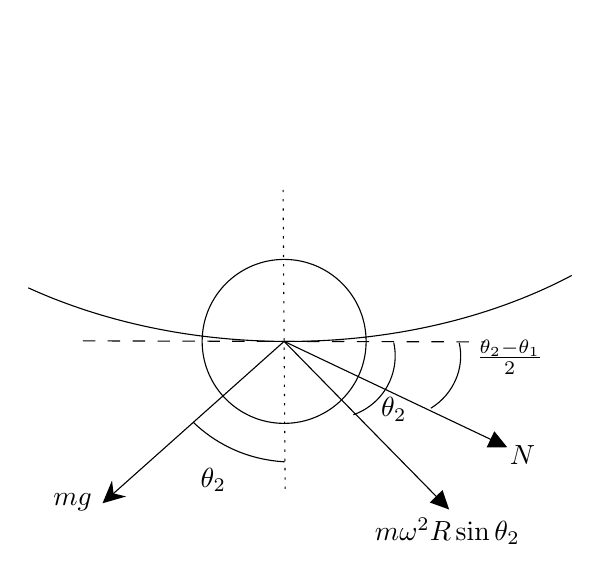
\begin{tikzpicture}[x=0.75pt,y=0.75pt,yscale=-1,xscale=1]
%uncomment if require: \path (0,300); %set diagram left start at 0, and has height of 300

%Shape: Circle [id:dp30092483561414674] 
\draw   (274,148.5) .. controls (274,126.68) and (291.68,109) .. (313.5,109) .. controls (335.32,109) and (353,126.68) .. (353,148.5) .. controls (353,170.32) and (335.32,188) .. (313.5,188) .. controls (291.68,188) and (274,170.32) .. (274,148.5) -- cycle ;
%Straight Lines [id:da04377590888362781] 
\draw  [dash pattern={on 4.5pt off 4.5pt}]  (216.5,148.25) -- (410.5,148.75) ;
%Straight Lines [id:da06469577602670684] 
\draw  [dash pattern={on 0.84pt off 2.51pt}]  (313,75.5) -- (314,221.5) ;
%Shape: Arc [id:dp8826917371364431] 
\draw  [draw opacity=0] (452.08,116.73) .. controls (413.85,136.96) and (365.53,148.88) .. (313.07,148.52) .. controls (267.6,148.21) and (225.37,138.72) .. (190.21,122.69) -- (314.1,-2.38) -- cycle ; \draw   (452.08,116.73) .. controls (413.85,136.96) and (365.53,148.88) .. (313.07,148.52) .. controls (267.6,148.21) and (225.37,138.72) .. (190.21,122.69) ;
%Straight Lines [id:da237751676993887] 
\draw    (313.5,148.5) -- (228.24,224.5) ;
\draw [shift={(226,226.5)}, rotate = 318.28999999999996] [fill={rgb, 255:red, 0; green, 0; blue, 0 }  ][line width=0.08]  [draw opacity=0] (10.72,-5.15) -- (0,0) -- (10.72,5.15) -- (7.12,0) -- cycle    ;
%Straight Lines [id:da5943969982079365] 
\draw    (313.5,148.5) -- (390.9,227.36) ;
\draw [shift={(393,229.5)}, rotate = 225.54] [fill={rgb, 255:red, 0; green, 0; blue, 0 }  ][line width=0.08]  [draw opacity=0] (8.93,-4.29) -- (0,0) -- (8.93,4.29) -- cycle    ;
%Straight Lines [id:da9852939397478429] 
\draw    (313.5,148.5) -- (418.29,198.21) ;
\draw [shift={(421,199.5)}, rotate = 205.38] [fill={rgb, 255:red, 0; green, 0; blue, 0 }  ][line width=0.08]  [draw opacity=0] (8.93,-4.29) -- (0,0) -- (8.93,4.29) -- cycle    ;
%Shape: Arc [id:dp03021420885503945] 
\draw  [draw opacity=0] (313.73,206.52) .. controls (304.47,205.99) and (295.48,203.74) .. (287.05,199.61) .. controls (280.61,196.46) and (274.84,192.37) .. (269.75,187.5) -- (344.78,81.73) -- cycle ; \draw   (313.73,206.52) .. controls (304.47,205.99) and (295.48,203.74) .. (287.05,199.61) .. controls (280.61,196.46) and (274.84,192.37) .. (269.75,187.5) ;
%Shape: Arc [id:dp5414323584167515] 
\draw  [draw opacity=0] (366.31,149.09) .. controls (367.17,152.99) and (367.26,157.13) .. (366.43,161.3) .. controls (364.3,172.14) and (356.58,180.45) .. (346.85,183.84) -- (337,155.5) -- cycle ; \draw   (366.31,149.09) .. controls (367.17,152.99) and (367.26,157.13) .. (366.43,161.3) .. controls (364.3,172.14) and (356.58,180.45) .. (346.85,183.84) ;
%Shape: Arc [id:dp19752711436542936] 
\draw  [draw opacity=0] (397.85,149.19) .. controls (400.65,161.37) and (395.04,174.05) .. (384.2,180.69) -- (368.67,156.1) -- cycle ; \draw   (397.85,149.19) .. controls (400.65,161.37) and (395.04,174.05) .. (384.2,180.69) ;

% Text Node
\draw (201,220.4) node [anchor=north west][inner sep=0.75pt]    {$mg$};
% Text Node
\draw (272,208.4) node [anchor=north west][inner sep=0.75pt]    {$\theta _{2}$};
% Text Node
\draw (359,174.4) node [anchor=north west][inner sep=0.75pt]    {$\theta _{2}$};
% Text Node
\draw (404.85,146.59) node [anchor=north west][inner sep=0.75pt]    {$\frac{\theta _{2} -\theta _{1}}{2}$};
% Text Node
\draw (356,232.4) node [anchor=north west][inner sep=0.75pt]    {$m\omega ^{2} R\sin \theta _{2}$};
% Text Node
\draw (421,197.4) node [anchor=north west][inner sep=0.75pt]    {$N$};


\end{tikzpicture}
\end{center}



\begin{center}
    $$ N \cos{\frac{\theta_1-\theta_2}{2}} =  mg\sin{\theta_2}- m {\omega}^2 R \sin{\theta_2}\cos{\theta_2}$$

$$m\omega^2 R \sin{\theta_1}\cos{\theta_1} - mg\sin{\theta_1} = mg\sin{\theta_2}- m {\omega}^2 R \sin{\theta_2}\cos{\theta_2}$$

\end{center}
\begin{center}

After solving, we get 
$\boxed{\theta_1 = 55\degree}$
and 
$\boxed{\theta_2 = 65\degree}$\\
\end{center}
\vspace{5pt}


\begin{center}
    

So, 
$\boxed{\frac{\theta_1 +3\theta_2}{50}}=5$
\end{center}
Note that we can also directly find the position of centre of mass of the two balls to find the angles easily.
\end{solution}
\vspace{10mm}%\section{Problem 4}


\begin{problem}
\begin{center}
    \textbf{The bouncing container}
\end{center}

There is a container containing two circular discs (of radii $0.5\ mm$ and $1\ mm$ respectively) which are connected by two light rigid rods of negligible area. The space between them is filled by a unknown ideal liquid, This container is dropped vertically on a table from a height $20 cm$, with which it in-elastically collides. Assume that the container loses all its kinetic energy into rest. It remains at rest for a time $t$ seconds and then it amazingly shoots back up to the same height 

Report value of $\boxed{10\cdot t}$ in seconds (round off to nearest integer).\newline

Neglect the hydro-static pressure of the liquid, assume pressure everywhere outside the space between the two discs to be ambient pressure $10^5 Pa$. Neglect all types of frictional forces i.e the discs are free to move up and down. The mass of the disc liquid system is $15\ g$. Assume the container is large enough so that the bottom piston don't fall out and also  the top piston does not reach the conical middle. \textbf{Assume the conical Portion of the container is small}

\begin{center}
    

\tikzset{every picture/.style={line width=0.75pt}} %set default line width to 0.75pt        

\begin{tikzpicture}[x=0.75pt,y=0.75pt,yscale=-1,xscale=1]
%uncomment if require: \path (0,666); %set diagram left start at 0, and has height of 666

%Shape: Rectangle [id:dp6765922522265879] 
\draw   (224.33,315) -- (415.33,315) -- (415.33,333) -- (224.33,333) -- cycle ;
%Straight Lines [id:da6762730467412184] 
\draw    (263.67,212.33) -- (224.33,315) ;
%Straight Lines [id:da46679514246897047] 
\draw    (415.33,315) -- (377,211.67) ;
%Straight Lines [id:da3821954840763684] 
\draw    (263.67,83) -- (263.67,212.33) ;
%Straight Lines [id:da31699044979410873] 
\draw    (377,82.33) -- (377,211.67) ;
%Straight Lines [id:da8140990384107647] 
\draw    (263.33,91.33) -- (376.33,91.33) ;
%Straight Lines [id:da9661505890772815] 
\draw    (264,110.67) -- (377,110.67) ;
%Straight Lines [id:da6542258080751477] 
\draw    (330.67,110.67) -- (330.67,314.33) ;
%Straight Lines [id:da6460986980892025] 
\draw    (342,111) -- (342,313.67) ;
%Straight Lines [id:da05134560291022505] 
\draw    (298,110.67) -- (298,314.33) ;
%Straight Lines [id:da3040956608276728] 
\draw    (309.33,111) -- (309.33,314.67) ;
%Straight Lines [id:da18253740333472201] 
\draw    (224.33,333) -- (224.33,432.33) ;
%Straight Lines [id:da48686026388239956] 
\draw    (415.33,333) -- (415.33,432.33) ;
%Straight Lines [id:da666427713195884] 
\draw    (320.5,78.33) -- (374,78.33) ;
\draw [shift={(377,78.33)}, rotate = 180] [fill={rgb, 255:red, 0; green, 0; blue, 0 }  ][line width=0.08]  [draw opacity=0] (8.93,-4.29) -- (0,0) -- (8.93,4.29) -- cycle    ;
%Straight Lines [id:da8499925094065273] 
\draw    (321.83,347) -- (410.67,347) ;
\draw [shift={(413.67,347)}, rotate = 180] [fill={rgb, 255:red, 0; green, 0; blue, 0 }  ][line width=0.08]  [draw opacity=0] (8.93,-4.29) -- (0,0) -- (8.93,4.29) -- cycle    ;
%Straight Lines [id:da11394745303626541] 
\draw    (395.67,87.33) -- (395.67,210.67) ;
\draw [shift={(395.67,213.67)}, rotate = 270] [fill={rgb, 255:red, 0; green, 0; blue, 0 }  ][line width=0.08]  [draw opacity=0] (8.93,-4.29) -- (0,0) -- (8.93,4.29) -- cycle    ;
\draw [shift={(395.67,84.33)}, rotate = 90] [fill={rgb, 255:red, 0; green, 0; blue, 0 }  ][line width=0.08]  [draw opacity=0] (8.93,-4.29) -- (0,0) -- (8.93,4.29) -- cycle    ;
%Straight Lines [id:da04620270285330208] 
\draw    (441,318) -- (441,426.67) ;
\draw [shift={(441,429.67)}, rotate = 270] [fill={rgb, 255:red, 0; green, 0; blue, 0 }  ][line width=0.08]  [draw opacity=0] (8.93,-4.29) -- (0,0) -- (8.93,4.29) -- cycle    ;
\draw [shift={(441,315)}, rotate = 90] [fill={rgb, 255:red, 0; green, 0; blue, 0 }  ][line width=0.08]  [draw opacity=0] (8.93,-4.29) -- (0,0) -- (8.93,4.29) -- cycle    ;

% Text Node
\draw (325.33,59.07) node [anchor=north west][inner sep=0.75pt]  [font=\small]  {$0.5mm$};
% Text Node
\draw (350.67,350.73) node [anchor=north west][inner sep=0.75pt]  [font=\small]  {$1mm$};
% Text Node
\draw (412,144.73) node [anchor=north west][inner sep=0.75pt]  [font=\small]  {$Large\ enough$};
% Text Node
\draw (458,365.4) node [anchor=north west][inner sep=0.75pt]  [font=\small]  {$Large\ enough$};


\end{tikzpicture}

\end{center}
\end{problem}
\begin{flushright}
\textbf{\Large{-Proposed by Abhiram Cherukupalli}}
\end{flushright}
\begin{solution}

{\Large{\textbf{Answer: 7}}}\\

The assumption here was to take conical section was of negligible height.\newline

When the impact happens the container comes to rest, but the pistons continue moving, since upper piston has lower area the pistons moving down will cause the volume between them to increase. As the liquid is in compressible, a vacuum will form between the pistons and the force due to pressure difference will provide the necessary impulse for bouncing.
Say $\Delta A$ is the difference in area of the pistons and $M_{total}$ is the total mass of the system then:

The upward force acting on the \textbf{water $+$ disc} system is:-
$$F=\Delta A P_0 - M_{total}\ g$$ 
Impulse equation
$$F\cdot t  = 2M_{total}\sqrt{2gh}$$

$$t = \frac{2M_{total}\sqrt{2gh}}{\Delta A P_0 - M_{total}\ g} \approx 0.7$$

\end{solution}
\vspace{10mm}%\section{Problem 5}
%hello

\begin{problem}

There is a superconducting ring,made up of perfectly conducting wire of mean radius $r=2m$ and cross-sectional area $A$ and of mass $10kg$ which floats in a gravity free space in a region of uniform magnetic field parallel to its induction vector  $\vec{B}=2T$. Inductance $L$ of the ring is so small that inertia of free electrons cannot be neglected in the current building process. The free electron density in the conductor is $n$, mass of an electron is $m_{e}$ and modulus of charge on an electron is $e$.He found that if the ring is turned slightly about a diameter and released, it will execute simple harmonic motion.If calculated time period is in form of \[\frac{\sqrt{a\left(L+\frac{ b \pi m_e}{ne^2 A}\right)}}{c}\] 
Find the value of $a+b-c$.


\begin{center}
    

\tikzset{every picture/.style={line width=0.75pt}} %set default line width to 0.75pt        

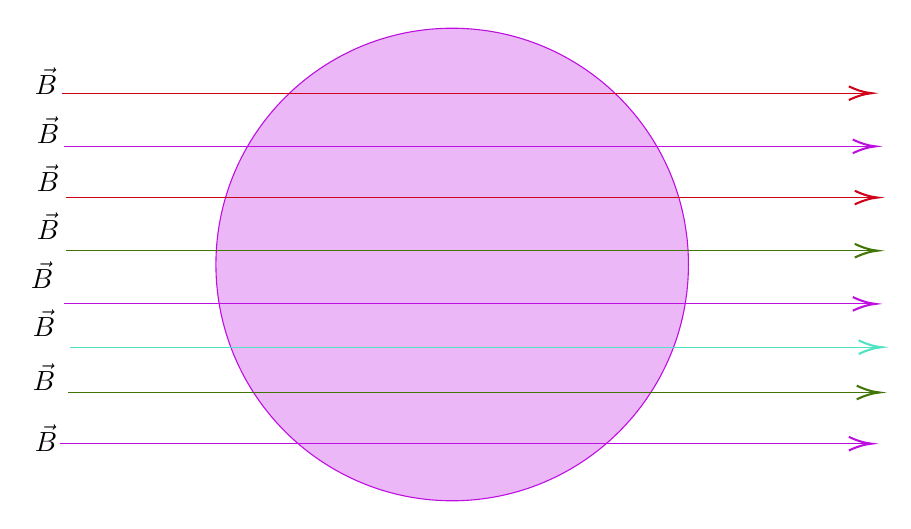
\begin{tikzpicture}[x=0.75pt,y=0.75pt,yscale=-1,xscale=1]
%uncomment if require: \path (0,445); %set diagram left start at 0, and has height of 445

%Shape: Ellipse [id:dp05979467864122956] 
\draw  [color={rgb, 255:red, 189; green, 16; blue, 224 }  ,draw opacity=1 ][fill={rgb, 255:red, 189; green, 16; blue, 224 }  ,fill opacity=0.3 ] (174.37,152.83) .. controls (174.37,89.97) and (225.33,39) .. (288.2,39) .. controls (351.07,39) and (402.03,89.97) .. (402.03,152.83) .. controls (402.03,215.7) and (351.07,266.67) .. (288.2,266.67) .. controls (225.33,266.67) and (174.37,215.7) .. (174.37,152.83) -- cycle ;
%Straight Lines [id:da38036810687504596] 
\draw [color={rgb, 255:red, 208; green, 2; blue, 27 }  ,draw opacity=1 ]   (100.37,70.3) -- (488.26,70.3) ;
\draw [shift={(490.26,70.3)}, rotate = 180] [color={rgb, 255:red, 208; green, 2; blue, 27 }  ,draw opacity=1 ][line width=0.75]    (10.93,-3.29) .. controls (6.95,-1.4) and (3.31,-0.3) .. (0,0) .. controls (3.31,0.3) and (6.95,1.4) .. (10.93,3.29)   ;
%Straight Lines [id:da2601477087726418] 
\draw [color={rgb, 255:red, 189; green, 16; blue, 224 }  ,draw opacity=1 ]   (101.32,95.92) -- (490.15,95.92) ;
\draw [shift={(492.15,95.92)}, rotate = 180] [color={rgb, 255:red, 189; green, 16; blue, 224 }  ,draw opacity=1 ][line width=0.75]    (10.93,-3.29) .. controls (6.95,-1.4) and (3.31,-0.3) .. (0,0) .. controls (3.31,0.3) and (6.95,1.4) .. (10.93,3.29)   ;
%Straight Lines [id:da10530259847828582] 
\draw [color={rgb, 255:red, 208; green, 2; blue, 27 }  ,draw opacity=1 ]   (102.27,120.58) -- (491.1,120.58) ;
\draw [shift={(493.1,120.58)}, rotate = 180] [color={rgb, 255:red, 208; green, 2; blue, 27 }  ,draw opacity=1 ][line width=0.75]    (10.93,-3.29) .. controls (6.95,-1.4) and (3.31,-0.3) .. (0,0) .. controls (3.31,0.3) and (6.95,1.4) .. (10.93,3.29)   ;
%Straight Lines [id:da07193348558462631] 
\draw [color={rgb, 255:red, 65; green, 117; blue, 5 }  ,draw opacity=1 ]   (102.27,146.19) -- (491.1,146.19) ;
\draw [shift={(493.1,146.19)}, rotate = 180] [color={rgb, 255:red, 65; green, 117; blue, 5 }  ,draw opacity=1 ][line width=0.75]    (10.93,-3.29) .. controls (6.95,-1.4) and (3.31,-0.3) .. (0,0) .. controls (3.31,0.3) and (6.95,1.4) .. (10.93,3.29)   ;
%Straight Lines [id:da4243731781989719] 
\draw [color={rgb, 255:red, 189; green, 16; blue, 224 }  ,draw opacity=1 ]   (101.32,171.81) -- (490.15,171.81) ;
\draw [shift={(492.15,171.81)}, rotate = 180] [color={rgb, 255:red, 189; green, 16; blue, 224 }  ,draw opacity=1 ][line width=0.75]    (10.93,-3.29) .. controls (6.95,-1.4) and (3.31,-0.3) .. (0,0) .. controls (3.31,0.3) and (6.95,1.4) .. (10.93,3.29)   ;
%Straight Lines [id:da47136077118995856] 
\draw [color={rgb, 255:red, 80; green, 227; blue, 194 }  ,draw opacity=1 ]   (104.17,192.68) -- (493,192.68) ;
\draw [shift={(495,192.68)}, rotate = 180] [color={rgb, 255:red, 80; green, 227; blue, 194 }  ,draw opacity=1 ][line width=0.75]    (10.93,-3.29) .. controls (6.95,-1.4) and (3.31,-0.3) .. (0,0) .. controls (3.31,0.3) and (6.95,1.4) .. (10.93,3.29)   ;
%Straight Lines [id:da709485033729087] 
\draw [color={rgb, 255:red, 65; green, 117; blue, 5 }  ,draw opacity=1 ]   (103.22,214.5) -- (492.05,214.5) ;
\draw [shift={(494.05,214.5)}, rotate = 180] [color={rgb, 255:red, 65; green, 117; blue, 5 }  ,draw opacity=1 ][line width=0.75]    (10.93,-3.29) .. controls (6.95,-1.4) and (3.31,-0.3) .. (0,0) .. controls (3.31,0.3) and (6.95,1.4) .. (10.93,3.29)   ;
%Straight Lines [id:da7157982471288351] 
\draw [color={rgb, 255:red, 189; green, 16; blue, 224 }  ,draw opacity=1 ]   (99.42,239.16) -- (488.26,239.16) ;
\draw [shift={(490.26,239.16)}, rotate = 180] [color={rgb, 255:red, 189; green, 16; blue, 224 }  ,draw opacity=1 ][line width=0.75]    (10.93,-3.29) .. controls (6.95,-1.4) and (3.31,-0.3) .. (0,0) .. controls (3.31,0.3) and (6.95,1.4) .. (10.93,3.29)   ;

% Text Node
\draw (85.83,56.86) node [anchor=north west][inner sep=0.75pt]    {$\vec{B}$};
% Text Node
\draw (86.78,80.17) node [anchor=north west][inner sep=0.75pt]    {$\vec{B}$};
% Text Node
\draw (86.78,103.47) node [anchor=north west][inner sep=0.75pt]    {$\vec{B}$};
% Text Node
\draw (86.78,126.78) node [anchor=north west][inner sep=0.75pt]    {$\vec{B}$};
% Text Node
\draw (83.94,150.09) node [anchor=north west][inner sep=0.75pt]    {$\vec{B}$};
% Text Node
\draw (84.89,199.54) node [anchor=north west][inner sep=0.75pt]    {$\vec{B}$};
% Text Node
\draw (84.89,173.4) node [anchor=north west][inner sep=0.75pt]    {$\vec{B}$};
% Text Node
\draw (85.83,228.54) node [anchor=north west][inner sep=0.75pt]    {$\vec{B}$};


\end{tikzpicture}

\end{center}
\end{problem}
\begin{flushright}
\textbf{\Large{-Proposed by AKIII}}
\end{flushright}
\begin{solution}

{\Large{\textbf{Answer: 7}}}\\


\textbf{Concept}: Given Inductance L of super conducting ring is so small that inductance due to free electrons cannot be ignored.\\


\begin{center}
    


\tikzset{every picture/.style={line width=0.75pt}} %set default line width to 0.75pt        

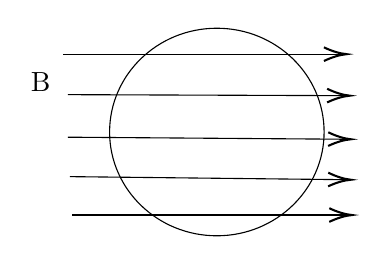
\begin{tikzpicture}[x=0.75pt,y=0.75pt,yscale=-1,xscale=1]
%uncomment if require: \path (0,300); %set diagram left start at 0, and has height of 300

%Shape: Ellipse [id:dp18773992959989738] 
\draw   (199.22,86) .. controls (199.22,58.39) and (222.35,36) .. (250.89,36) .. controls (279.43,36) and (302.57,58.39) .. (302.57,86) .. controls (302.57,113.61) and (279.43,136) .. (250.89,136) .. controls (222.35,136) and (199.22,113.61) .. (199.22,86) -- cycle ;
%Straight Lines [id:da7945784458785592] 
\draw    (177,48.5) -- (311.42,48.5) ;
\draw [shift={(313.42,48.5)}, rotate = 180] [color={rgb, 255:red, 0; green, 0; blue, 0 }  ][line width=0.75]    (10.93,-3.29) .. controls (6.95,-1.4) and (3.31,-0.3) .. (0,0) .. controls (3.31,0.3) and (6.95,1.4) .. (10.93,3.29)   ;
%Straight Lines [id:da07279399159825584] 
\draw    (179.07,68) -- (312.97,68.49) ;
\draw [shift={(314.97,68.5)}, rotate = 180.21] [color={rgb, 255:red, 0; green, 0; blue, 0 }  ][line width=0.75]    (10.93,-3.29) .. controls (6.95,-1.4) and (3.31,-0.3) .. (0,0) .. controls (3.31,0.3) and (6.95,1.4) .. (10.93,3.29)   ;
%Straight Lines [id:da6554245998310364] 
\draw    (179.07,88.5) -- (313.48,89.49) ;
\draw [shift={(315.48,89.5)}, rotate = 180.42] [color={rgb, 255:red, 0; green, 0; blue, 0 }  ][line width=0.75]    (10.93,-3.29) .. controls (6.95,-1.4) and (3.31,-0.3) .. (0,0) .. controls (3.31,0.3) and (6.95,1.4) .. (10.93,3.29)   ;
%Straight Lines [id:da6826987392486712] 
\draw    (180.1,107.5) -- (313.48,108.98) ;
\draw [shift={(315.48,109)}, rotate = 180.63] [color={rgb, 255:red, 0; green, 0; blue, 0 }  ][line width=0.75]    (10.93,-3.29) .. controls (6.95,-1.4) and (3.31,-0.3) .. (0,0) .. controls (3.31,0.3) and (6.95,1.4) .. (10.93,3.29)   ;
%Straight Lines [id:da18402007065782544] 
\draw    (181.13,126) -- (314,126) ;
\draw [shift={(316,126)}, rotate = 180] [color={rgb, 255:red, 0; green, 0; blue, 0 }  ][line width=0.75]    (10.93,-3.29) .. controls (6.95,-1.4) and (3.31,-0.3) .. (0,0) .. controls (3.31,0.3) and (6.95,1.4) .. (10.93,3.29)   ;

% Text Node

\draw (160.02,56.25) node [anchor=north west][inner sep=0.75pt]   [align=left] {B};
\end{tikzpicture}
      
      
      

  \end{center}



We'll use the concept of Kinetic inductance. \\
Here, $L'$ is the kinetic inductance. 

Kinetic energy of electron $= \frac{1}{2} L' i^2 \implies \frac{1}{2} M v_{e}^{2} = \frac{1}{2} L' i^2$
Now, we know, $i = neA v_d \implies v_d = \frac{i}{neA}$ \\
Also, by definition, $M = n m_e A \cdot 2 \pi R$ \\
Hence, from our previous equation, we can write 
\[\frac{1}{2} n m_e A \cdot 2 \pi R \frac{i^2}{n^2 e^2 A^2} = \frac{1}{2} L' i^2 \implies \boxed{L' = \frac{2 \pi R m_e}{n e^2 A}}\] \\

So, $L_{\text{net}} = L + L'$
Now the ring is rotated by a small angle, we can calculate the torque $\tau$ due to the magnetic field : \\
\[\tau = \pi R^2 \cdot i B \cos \theta = \frac{B^2 \sin \theta \cos \theta (\pi R^2)^2 }{L_{net}}\]



\centering
\tikzset{every picture/.style={line width=0.75pt}} %set default line width to 0.75pt        

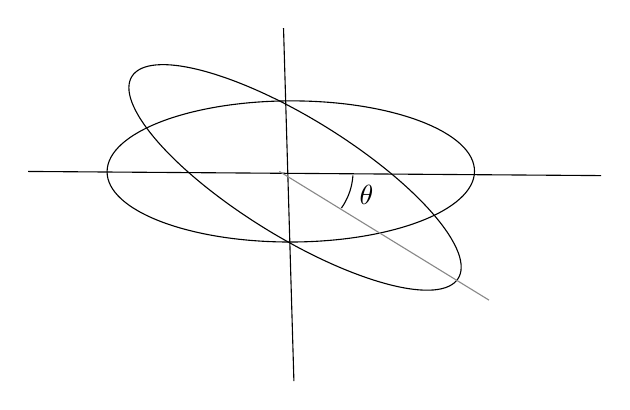
\begin{tikzpicture}[x=0.75pt,y=0.75pt,yscale=-1,xscale=1]
%uncomment if require: \path (0,300); %set diagram left start at 0, and has height of 300

%Straight Lines [id:da9132170475409473] 
\draw    (293,80) -- (298,250) ;
%Straight Lines [id:da904132178602624] 
\draw    (170,149) -- (446,151) ;
%Shape: Ellipse [id:dp46793606097635765] 
\draw   (207.99,149) .. controls (208.2,130.22) and (248,115) .. (296.88,115) .. controls (345.76,115) and (385.22,130.22) .. (385.01,149) .. controls (384.8,167.78) and (345,183) .. (296.12,183) .. controls (247.24,183) and (207.78,167.78) .. (207.99,149) -- cycle ;
%Shape: Ellipse [id:dp9743768144737246] 
\draw   (332.89,200.16) .. controls (292.96,186.41) and (245.22,153.64) .. (226.25,126.97) .. controls (207.29,100.3) and (224.28,89.84) .. (264.21,103.59) .. controls (304.13,117.35) and (351.87,150.12) .. (370.84,176.78) .. controls (389.8,203.45) and (372.81,213.92) .. (332.89,200.16) -- cycle ;
%Straight Lines [id:da5488554350772532] 
\draw [color={rgb, 255:red, 136; green, 136; blue, 136 }  ,draw opacity=1 ]   (291,149) -- (392,211) ;
%Shape: Arc [id:dp0894816958911715] 
\draw  [draw opacity=0] (320.9,166.65) .. controls (323.69,162.69) and (325.59,157.99) .. (326.26,152.82) .. controls (326.34,152.18) and (326.4,151.54) .. (326.44,150.9) -- (296.5,149) -- cycle ; \draw   (320.9,166.65) .. controls (323.69,162.69) and (325.59,157.99) .. (326.26,152.82) .. controls (326.34,152.18) and (326.4,151.54) .. (326.44,150.9) ;

% Text Node
\draw (328.44,154.3) node [anchor=north west][inner sep=0.75pt]    {$\theta $};


\end{tikzpicture}



Since its a super conducting ring, flux is constant thus, $\boxed{L_{net} i = B \sin \theta \pi R^2}$ \\
\vspace{0.4mm}

Hence for small angle $\theta$, S.H.M. : \\

\[T= 2 \pi \sqrt{\frac{\frac{mR^2}{2}L_{net}}{B^2 (\pi R^2)^2}} = \frac{2}{BR} \sqrt{\frac{m L_{net}}{2}} = \frac{\sqrt{2m L_{net}}}{BR}\]



\end{solution}
\vspace{10mm}%\section{Problem 6}

\begin{problem}
 
A square loop of negligible resistance, side length $10\ cm$, mass $0.9g$, total self inductance $4\cdot 10^{-8} H$ is left in a vertical plane where where its bottom end touches the interface of two different uniform horizontal magnetic fields ($B_{upper}>B_{lower}$) where $B_{upper}=1.5mT\ \hat{k}$ and $B_{lower}=0.6mT\ \hat{k}$. There is also a drag force, $f=-kv\ \ (k=1.8\cdot10^{-6})$ acting on it. This square loop happens to undergo a damped simple harmonic motion, mark the correct options:
\begin{enumerate}[label=\Alph*]
%\item The damping coefficient of the resulting oscillations $\gamma$ is $10^{-3} \ Ns/m$
\item The damping coefficient of the resulting oscillations $\gamma$ is $1.5\cdot 10^{-3}\ Ns/m$
%\item The angular frequency omega of the oscillations $\omega$ is  $5\ rad/s$
\item The angular frequency omega of the oscillations $\omega$ is  $10\ rad/s$
\item The maximum magnetic field of the lower region for SHM to ensue is $9\cdot 10^{-4} T$
\item The vertical position $z(t)\approx 0.1\left(1-\frac{e^{0.0015t}}{\cos \phi}\left(cos\left(5t-\phi\right)\right)\right)$, $\phi=\arctan(\frac{\gamma}{\sqrt{\omega^2-\gamma^2}})$ \newline \newline 

%item The vertical displacement $z(t)$ at $t=50s$ is approximately $0.31\ m$\newline (Useful values: $cos(250)\approx0.75,\ e^{-0.075}\approx0.93,\ e^{-0.05}\approx0.95$, $\phi \to 0$)
\end{enumerate}



\begin{center}
    

\tikzset{every picture/.style={line width=0.75pt}} %set default line width to 0.75pt        

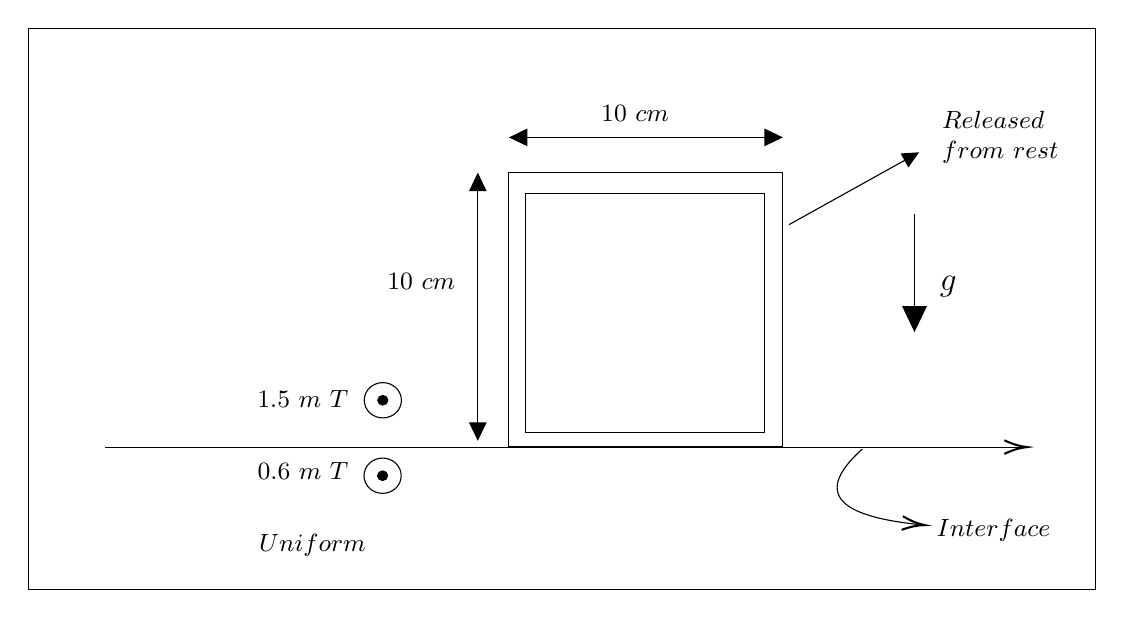
\begin{tikzpicture}[x=0.75pt,y=0.75pt,yscale=-1,xscale=1]
%uncomment if require: \path (0,342); %set diagram left start at 0, and has height of 342

%Shape: Square [id:dp5229399275176978] 
\draw   (295.4,79.8) -- (427.4,79.8) -- (427.4,211.8) -- (295.4,211.8) -- cycle ;
%Shape: Square [id:dp3120302301077711] 
\draw   (303.4,89.8) -- (418.4,89.8) -- (418.4,204.8) -- (303.4,204.8) -- cycle ;
%Straight Lines [id:da4295345134083759] 
\draw    (490.8,99.8) -- (490.8,153.6) ;
\draw [shift={(490.8,156.6)}, rotate = 270] [fill={rgb, 255:red, 0; green, 0; blue, 0 }  ][line width=0.08]  [draw opacity=0] (12.5,-6.01) -- (0,0) -- (12.5,6.01) -- cycle    ;
%Shape: Ellipse [id:dp970810654059975] 
\draw   (225.57,225.8) .. controls (225.57,230.49) and (229.58,234.3) .. (234.53,234.3) .. controls (239.48,234.3) and (243.49,230.49) .. (243.49,225.8) .. controls (243.49,221.11) and (239.48,217.3) .. (234.53,217.3) .. controls (229.58,217.3) and (225.57,221.11) .. (225.57,225.8) -- cycle ;
%Shape: Ellipse [id:dp5337405225219265] 
\draw  [fill={rgb, 255:red, 0; green, 0; blue, 0 }  ,fill opacity=1 ] (232.11,225.8) .. controls (232.11,227.07) and (233.2,228.1) .. (234.53,228.1) .. controls (235.87,228.1) and (236.95,227.07) .. (236.95,225.8) .. controls (236.95,224.53) and (235.87,223.5) .. (234.53,223.5) .. controls (233.2,223.5) and (232.11,224.53) .. (232.11,225.8) -- cycle ;


%Shape: Ellipse [id:dp5355560509346897] 
\draw   (225.69,189.45) .. controls (225.69,194.14) and (229.7,197.95) .. (234.64,197.95) .. controls (239.59,197.95) and (243.6,194.14) .. (243.6,189.45) .. controls (243.6,184.76) and (239.59,180.95) .. (234.64,180.95) .. controls (229.7,180.95) and (225.69,184.76) .. (225.69,189.45) -- cycle ;
%Shape: Ellipse [id:dp02522629369216345] 
\draw  [fill={rgb, 255:red, 0; green, 0; blue, 0 }  ,fill opacity=1 ] (232.22,189.45) .. controls (232.22,190.72) and (233.31,191.75) .. (234.64,191.75) .. controls (235.98,191.75) and (237.06,190.72) .. (237.06,189.45) .. controls (237.06,188.18) and (235.98,187.15) .. (234.64,187.15) .. controls (233.31,187.15) and (232.22,188.18) .. (232.22,189.45) -- cycle ;


%Straight Lines [id:da08588954936767434] 
\draw    (298.4,62.8) -- (424.4,62.8) ;
\draw [shift={(427.4,62.8)}, rotate = 180] [fill={rgb, 255:red, 0; green, 0; blue, 0 }  ][line width=0.08]  [draw opacity=0] (8.93,-4.29) -- (0,0) -- (8.93,4.29) -- cycle    ;
\draw [shift={(295.4,62.8)}, rotate = 0] [fill={rgb, 255:red, 0; green, 0; blue, 0 }  ][line width=0.08]  [draw opacity=0] (8.93,-4.29) -- (0,0) -- (8.93,4.29) -- cycle    ;
%Curve Lines [id:da7595553637659127] 
\draw    (465.6,213) .. controls (438.61,237.23) and (460.72,246.13) .. (494.26,249.45) ;
\draw [shift={(495.8,249.6)}, rotate = 185.31] [color={rgb, 255:red, 0; green, 0; blue, 0 }  ][line width=0.75]    (10.93,-3.29) .. controls (6.95,-1.4) and (3.31,-0.3) .. (0,0) .. controls (3.31,0.3) and (6.95,1.4) .. (10.93,3.29)   ;
%Shape: Rectangle [id:dp45327494038566263] 
\draw   (63.8,10.2) -- (578.2,10.2) -- (578.2,280.6) -- (63.8,280.6) -- cycle ;
%Straight Lines [id:da1292145509412892] 
\draw    (101,212) -- (543,212) ;
\draw [shift={(545,212)}, rotate = 180] [color={rgb, 255:red, 0; green, 0; blue, 0 }  ][line width=0.75]    (10.93,-3.29) .. controls (6.95,-1.4) and (3.31,-0.3) .. (0,0) .. controls (3.31,0.3) and (6.95,1.4) .. (10.93,3.29)   ;
%Straight Lines [id:da05076878982883226] 
\draw    (430.4,104.8) -- (490.38,71.46) ;
\draw [shift={(493,70)}, rotate = 510.93] [fill={rgb, 255:red, 0; green, 0; blue, 0 }  ][line width=0.08]  [draw opacity=0] (8.04,-3.86) -- (0,0) -- (8.04,3.86) -- cycle    ;
%Straight Lines [id:da22790768373888048] 
\draw    (280.4,82.8) -- (280.4,206) ;
\draw [shift={(280.4,209)}, rotate = 270] [fill={rgb, 255:red, 0; green, 0; blue, 0 }  ][line width=0.08]  [draw opacity=0] (8.93,-4.29) -- (0,0) -- (8.93,4.29) -- cycle    ;
\draw [shift={(280.4,79.8)}, rotate = 90] [fill={rgb, 255:red, 0; green, 0; blue, 0 }  ][line width=0.08]  [draw opacity=0] (8.93,-4.29) -- (0,0) -- (8.93,4.29) -- cycle    ;

% Text Node
\draw (501.8,128.2) node [anchor=north west][inner sep=0.75pt]  [font=\large]  {$g$};
% Text Node
\draw (338.6,51.05) node [anchor=west] [inner sep=0.75pt]  [font=\small]  {$10\ cm$};
% Text Node
\draw (500.2,251.85) node [anchor=west] [inner sep=0.75pt]  [font=\small]  {$Interface$};
% Text Node
\draw (173.78,259.37) node [anchor=west] [inner sep=0.75pt]  [font=\small]  {$Uniform$};
% Text Node
\draw (172.96,188.69) node [anchor=west] [inner sep=0.75pt]  [font=\small]  {$1.5\ m\ T$};
% Text Node
\draw (173.07,218.1) node [anchor=north west][inner sep=0.75pt]  [font=\small]  {$0.6\ m\ T$};
% Text Node
\draw (496.2,62.85) node [anchor=west] [inner sep=0.75pt]  [font=\small]  {$ \begin{array}{l}
Released\ \\
from\ rest
\end{array}$};
% Text Node
\draw (235.6,132.05) node [anchor=west] [inner sep=0.75pt]  [font=\small]  {$10\ cm$};


\end{tikzpicture}

\end{center}




\end{problem}
\begin{flushright}
\textbf{\Large{-Proposed by Abhiram Cherukupalli}}
\end{flushright}
\begin{solution}

 {\Large{\textbf{Answer: C}}}\\
 
 

\centering
\tikzset{every picture/.style={line width=0.75pt}} %set default line width to 0.75pt        

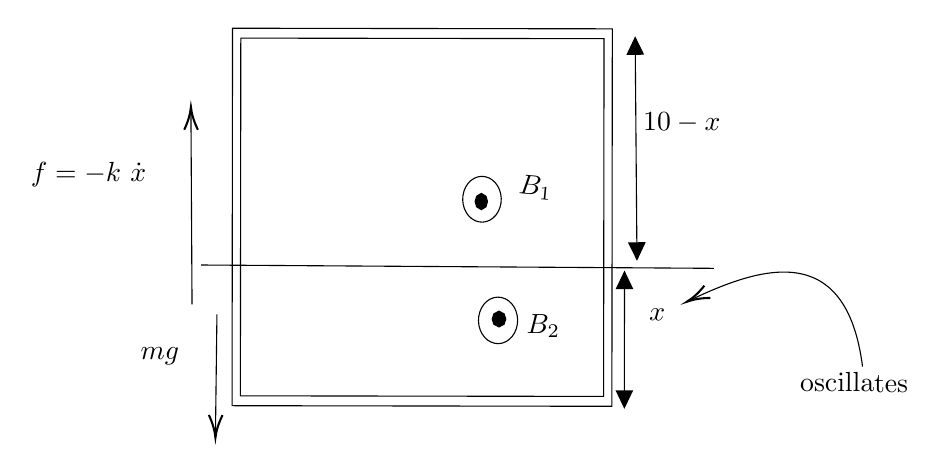
\begin{tikzpicture}[x=0.75pt,y=0.75pt,yscale=-1,xscale=1]
%uncomment if require: \path (0,241); %set diagram left start at 0, and has height of 241

%Straight Lines [id:da7999061003008845] 
\draw    (436.32,140.34) -- (189.32,138.74) ;
%Flowchart: Process [id:dp6807274744970491] 
\draw   (383.45,29.69) -- (383.23,202.05) -- (208.24,201.77) -- (208.45,29.42) -- cycle ;
%Straight Lines [id:da8174291039512145] 
\draw    (398.47,31.53) -- (399.3,133.71) ;
\draw [shift={(399.32,136.71)}, rotate = 269.54] [fill={rgb, 255:red, 0; green, 0; blue, 0 }  ][line width=0.08]  [draw opacity=0] (8.93,-4.29) -- (0,0) -- (8.93,4.29) -- cycle    ;
\draw [shift={(398.45,28.53)}, rotate = 89.54] [fill={rgb, 255:red, 0; green, 0; blue, 0 }  ][line width=0.08]  [draw opacity=0] (8.93,-4.29) -- (0,0) -- (8.93,4.29) -- cycle    ;
%Straight Lines [id:da38632814417785144] 
\draw    (393.31,144.45) -- (393.24,205.02) ;
\draw [shift={(393.24,208.02)}, rotate = 270.07] [fill={rgb, 255:red, 0; green, 0; blue, 0 }  ][line width=0.08]  [draw opacity=0] (8.93,-4.29) -- (0,0) -- (8.93,4.29) -- cycle    ;
\draw [shift={(393.31,141.45)}, rotate = 90.07] [fill={rgb, 255:red, 0; green, 0; blue, 0 }  ][line width=0.08]  [draw opacity=0] (8.93,-4.29) -- (0,0) -- (8.93,4.29) -- cycle    ;
%Shape: Ellipse [id:dp8775455151946339] 
\draw   (321.3,117.35) .. controls (316.51,115.15) and (314.14,108.76) .. (315.98,103.08) .. controls (317.83,97.4) and (323.21,94.57) .. (327.99,96.77) .. controls (332.77,98.96) and (335.15,105.35) .. (333.3,111.04) .. controls (331.45,116.72) and (326.08,119.55) .. (321.3,117.35) -- cycle ;
\draw  [line width=2.25]  (324.33,105.68) .. controls (325.26,105.68) and (326.01,106.79) .. (326.01,108.15) .. controls (326.01,109.52) and (325.25,110.63) .. (324.32,110.63) .. controls (323.39,110.62) and (322.64,109.51) .. (322.64,108.15) .. controls (322.64,106.78) and (323.4,105.68) .. (324.33,105.68) -- cycle ; \draw  [line width=2.25]  (324.33,105.68) -- (324.32,110.63) ; \draw  [line width=2.25]  (326.01,108.15) -- (322.64,108.15) ;
\draw  [line width=3]  (332.84,166.61) .. controls (333.64,166.61) and (334.29,165.79) .. (334.29,164.78) .. controls (334.29,163.77) and (333.64,162.95) .. (332.84,162.94) .. controls (332.04,162.94) and (331.39,163.76) .. (331.39,164.77) .. controls (331.39,165.79) and (332.04,166.61) .. (332.84,166.61) -- cycle ; \draw  [line width=3]  (332.84,166.61) -- (332.84,162.94) ; \draw  [line width=3]  (334.29,164.78) -- (331.39,164.77) ;
%Shape: Ellipse [id:dp6539858849154265] 
\draw   (328.99,175.87) .. controls (324.13,173.64) and (321.72,167.15) .. (323.59,161.38) .. controls (325.47,155.61) and (330.93,152.74) .. (335.79,154.97) .. controls (340.65,157.2) and (343.06,163.69) .. (341.18,169.46) .. controls (339.3,175.23) and (333.84,178.11) .. (328.99,175.87) -- cycle ;
%Straight Lines [id:da7257166116548053] 
\draw    (196.95,162.53) -- (196.24,219.96) ;
\draw [shift={(196.22,221.96)}, rotate = 270.7] [color={rgb, 255:red, 0; green, 0; blue, 0 }  ][line width=0.75]    (10.93,-3.29) .. controls (6.95,-1.4) and (3.31,-0.3) .. (0,0) .. controls (3.31,0.3) and (6.95,1.4) .. (10.93,3.29)   ;
%Straight Lines [id:da38400722113680597] 
\draw    (184.95,157.75) -- (184.42,64.65) ;
\draw [shift={(184.41,62.65)}, rotate = 449.67] [color={rgb, 255:red, 0; green, 0; blue, 0 }  ][line width=0.75]    (10.93,-3.29) .. controls (6.95,-1.4) and (3.31,-0.3) .. (0,0) .. controls (3.31,0.3) and (6.95,1.4) .. (10.93,3.29)   ;
%Shape: Rectangle [id:dp714959021762209] 
\draw   (387.45,24.95) -- (387.23,206.81) -- (204.24,206.52) -- (204.46,24.66) -- cycle ;
%Curve Lines [id:da054310102500288115] 
\draw    (508,187.66) .. controls (500.12,126.59) and (459.25,139.25) .. (424.95,155.67) ;
\draw [shift={(423.39,156.42)}, rotate = 334.15999999999997] [color={rgb, 255:red, 0; green, 0; blue, 0 }  ][line width=0.75]    (10.93,-3.29) .. controls (6.95,-1.4) and (3.31,-0.3) .. (0,0) .. controls (3.31,0.3) and (6.95,1.4) .. (10.93,3.29)   ;

% Text Node
\draw (401.06,63.93) node [anchor=north west][inner sep=0.75pt]  [rotate=-0.08]  {$10-x$};
% Text Node
\draw (404.17,158.67) node [anchor=north west][inner sep=0.75pt]  [rotate=-1.72]  {$x$};
% Text Node
\draw (341.86,93.85) node [anchor=north west][inner sep=0.75pt]  [rotate=-5.33]  {$B_{1}$};
% Text Node
\draw (344.95,161.31) node [anchor=north west][inner sep=0.75pt]  [rotate=-0.08]  {$B_{2}$};
% Text Node
\draw (158.88,177.4) node [anchor=north west][inner sep=0.75pt]    {$mg$};
% Text Node
\draw (106.03,87.81) node [anchor=north west][inner sep=0.75pt]    {$f=-k\ \dot{x}$};
% Text Node
\draw (476.79,189.18) node [anchor=north west][inner sep=0.75pt]  [rotate=-0.39] [align=left] {oscillates};


\end{tikzpicture}
 
 
 
 
 
 
Net flux passing through the loop:
$$\Phi = B_1 a^2+(B_1-B_2)ax+LI$$
$$\implies I\cdot R = -\frac{d\phi}{dt}=(B_1-B_2)a\dot{x}-L\dot{I}=0$$
$$\implies mg - m\dot{x}-(B_1-B_2)aI=m\ddot{x}$$

Differentiating and solving we get:

$$\ddot{x}+2\cdot \frac{1}{2}\frac{\eta}{m}\dot{x}+\frac{(B_1-B_2)^2a^2}{mL}x = g$$

Damping coefficient $\boxed{\gamma=\frac{1}{2}\frac{\eta}{m}=10^{-3}}$\newline
Angular frequency of oscillation $\boxed{\omega =\sqrt{\frac{(B_1-B_2)^2a^2}{mL}}=15 rad/s}$\newline
Vertical position as a function of time
$\boxed{z(t)=4.44\left(1-\frac{e^{0.001t}}{\cos \phi}(cos(15t-\phi))\right)cm}$\newline
               where $\phi=arctan(\frac{\gamma}{\sqrt{\omega^2-\gamma^2}})$
\newline
For SHM to ensue:
$$\frac{g}{\omega^2}<a\implies \left| B_1-B_2 \right|>0.6mT \implies \boxed{B_2<0.9mT}\ or \ B_2>2.1mT$$

But since $B_{upper}>B_{lower}$ we don't consider the second possibility as it is the best possible option.


\end{solution}
\vspace{10mm}%\section{Problem 7}

\begin{problem}

In this problem, we will be analysing the formation of image of ring around galaxies using Corpuscluar Theory and Universal Law of Gravitation. (Note: Do not consider any aspects of Relativity while solving this problem, i.e, solve it using only Classical Mechanics) 

\vspace{3mm}

Consider light as a collection of particles of mass m moving with a very high speed c ($c^2>>\frac{GM}{b}$, where $b$ is the impact parameter). These particles will deviate when they come under the interaction of a star as shown in figure. Consider a simple setup with one star acting as a lens. Let the distance of object and observer be $v$ and $u$ respectively. Mark the correct statements:


\begin{center}
    \tikzset{every picture/.style={line width=0.75pt}} %set default line width to 0.75pt        

\begin{tikzpicture}[x=0.75pt,y=0.75pt,yscale=-1,xscale=1]
%uncomment if require: \path (0,310); %set diagram left start at 0, and has height of 310

%Shape: Circle [id:dp8189008140498129] 
\draw   (300.25,159.95) .. controls (300.25,148.49) and (309.54,139.2) .. (321,139.2) .. controls (332.46,139.2) and (341.75,148.49) .. (341.75,159.95) .. controls (341.75,171.41) and (332.46,180.7) .. (321,180.7) .. controls (309.54,180.7) and (300.25,171.41) .. (300.25,159.95) -- cycle ;
%Straight Lines [id:da8578850848547468] 
\draw  [dash pattern={on 0.84pt off 2.51pt}]  (81,159.95) -- (519.5,159.95) ;
%Curve Lines [id:da6860115810578344] 
\draw    (81,159.95) .. controls (284.6,92.33) and (375.27,100.33) .. (519.5,159.95) ;
\draw [shift={(519.5,159.95)}, rotate = 22.46] [color={rgb, 255:red, 0; green, 0; blue, 0 }  ][fill={rgb, 255:red, 0; green, 0; blue, 0 }  ][line width=0.75]      (0, 0) circle [x radius= 3.35, y radius= 3.35]   ;
\draw [shift={(302.43,112.42)}, rotate = 357.73] [fill={rgb, 255:red, 0; green, 0; blue, 0 }  ][line width=0.08]  [draw opacity=0] (8.93,-4.29) -- (0,0) -- (8.93,4.29) -- cycle    ;
\draw [shift={(81,159.95)}, rotate = 341.63] [color={rgb, 255:red, 0; green, 0; blue, 0 }  ][fill={rgb, 255:red, 0; green, 0; blue, 0 }  ][line width=0.75]      (0, 0) circle [x radius= 3.35, y radius= 3.35]   ;
%Straight Lines [id:da2650778345953846] 
\draw  [dash pattern={on 0.84pt off 2.51pt}]  (81,159.95) -- (518.6,19.67) ;
\draw [shift={(518.6,19.67)}, rotate = 342.23] [color={rgb, 255:red, 0; green, 0; blue, 0 }  ][fill={rgb, 255:red, 0; green, 0; blue, 0 }  ][line width=0.75]      (0, 0) circle [x radius= 3.35, y radius= 3.35]   ;
%Straight Lines [id:da6424831992606801] 
\draw  [dash pattern={on 0.84pt off 2.51pt}]  (518.6,19.67) -- (519.5,159.95) ;
%Straight Lines [id:da7700477679799866] 
\draw  [dash pattern={on 0.84pt off 2.51pt}]  (321.25,114.67) -- (321.02,156.95) ;
\draw [shift={(321,159.95)}, rotate = 270.32] [fill={rgb, 255:red, 0; green, 0; blue, 0 }  ][line width=0.08]  [draw opacity=0] (8.93,-4.29) -- (0,0) -- (8.93,4.29) -- cycle    ;
\draw [shift={(321.27,111.67)}, rotate = 90.32] [fill={rgb, 255:red, 0; green, 0; blue, 0 }  ][line width=0.08]  [draw opacity=0] (8.93,-4.29) -- (0,0) -- (8.93,4.29) -- cycle    ;
%Straight Lines [id:da32502282430695995] 
\draw  [dash pattern={on 0.84pt off 2.51pt}]  (81.67,184.69) -- (314.93,186.31) ;
\draw [shift={(317.93,186.33)}, rotate = 180.4] [fill={rgb, 255:red, 0; green, 0; blue, 0 }  ][line width=0.08]  [draw opacity=0] (8.93,-4.29) -- (0,0) -- (8.93,4.29) -- cycle    ;
\draw [shift={(78.67,184.67)}, rotate = 0.4] [fill={rgb, 255:red, 0; green, 0; blue, 0 }  ][line width=0.08]  [draw opacity=0] (8.93,-4.29) -- (0,0) -- (8.93,4.29) -- cycle    ;
%Straight Lines [id:da11885840508405776] 
\draw  [dash pattern={on 0.84pt off 2.51pt}]  (328.33,187.99) -- (519.6,187.67) ;
\draw [shift={(522.6,187.67)}, rotate = 539.9] [fill={rgb, 255:red, 0; green, 0; blue, 0 }  ][line width=0.08]  [draw opacity=0] (8.93,-4.29) -- (0,0) -- (8.93,4.29) -- cycle    ;
\draw [shift={(325.33,188)}, rotate = 359.9] [fill={rgb, 255:red, 0; green, 0; blue, 0 }  ][line width=0.08]  [draw opacity=0] (8.93,-4.29) -- (0,0) -- (8.93,4.29) -- cycle    ;
%Shape: Arc [id:dp253616603242081] 
\draw  [draw opacity=0] (113.69,149.32) .. controls (113.75,149.45) and (113.8,149.57) .. (113.86,149.7) .. controls (115.34,152.99) and (116.18,156.4) .. (116.43,159.8) -- (86.5,162) -- cycle ; \draw   (113.69,149.32) .. controls (113.75,149.45) and (113.8,149.57) .. (113.86,149.7) .. controls (115.34,152.99) and (116.18,156.4) .. (116.43,159.8) ;
%Shape: Arc [id:dp5378466827484714] 
\draw  [draw opacity=0] (489.5,160.12) .. controls (489.5,159.65) and (489.51,159.17) .. (489.53,158.68) .. controls (489.68,155.08) and (490.46,151.65) .. (491.76,148.51) -- (519.5,159.95) -- cycle ; \draw   (489.5,160.12) .. controls (489.5,159.65) and (489.51,159.17) .. (489.53,158.68) .. controls (489.68,155.08) and (490.46,151.65) .. (491.76,148.51) ;

% Text Node
\draw (310.67,190.73) node [anchor=north west][inner sep=0.75pt]    {$M$};
% Text Node
\draw (528.67,73.73) node [anchor=north west][inner sep=0.75pt]    {$R$};
% Text Node
\draw (495.33,198) node [anchor=north west][inner sep=0.75pt]   [align=left] {Object};
% Text Node
\draw (88,216) node   [align=left] {\begin{minipage}[lt]{68pt}\setlength\topsep{0pt}
Observer
\end{minipage}};
% Text Node
\draw (328.67,123.07) node [anchor=north west][inner sep=0.75pt]    {$b$};
% Text Node
\draw (131,147.07) node [anchor=north west][inner sep=0.75pt]    {$\theta $};
% Text Node
\draw (178.67,191.4) node [anchor=north west][inner sep=0.75pt]    {$u$};
% Text Node
\draw (420.67,190.4) node [anchor=north west][inner sep=0.75pt]    {$v$};
% Text Node
\draw (290.67,214.4) node [anchor=north west][inner sep=0.75pt]    {$\theta ,\ \alpha \ll 1$};
% Text Node
\draw (464.42,146.57) node [anchor=north west][inner sep=0.75pt]    {$\alpha $};
% Text Node
\draw (528,12) node [anchor=north west][inner sep=0.75pt]   [align=left] {Image};


\end{tikzpicture}
\end{center}

\vspace{5mm}

\textbf{A)} The radius of ring observed will be $\sqrt{\frac{2GMv(u+v)}{c^2u}}$

\vspace{2mm}


\textbf{B)} The maximum radius of star which can create such a image is $\sqrt{\frac{4GMvu}{c^2(u+v)}}$

\vspace{2mm}

\textbf{C)} For $v>>u$, the value of angle subtended by ring at observer will be $\sqrt{\frac{4GM}{uc^2}}$

\vspace{2mm}

\textbf{D)} The value of $\alpha+\theta$ is $\frac{2GM}{bc^2}$
\end{problem}
\begin{flushright}
\textbf{\Large{-Proposed by Prerak}}
\end{flushright}
\begin{solution}
  {\Large{\textbf{Answers: (A), (D)}}}\\
First, let's find the deviation angle for impact parameter "b"

\begin{center}
    

\tikzset{every picture/.style={line width=0.75pt}} %set default line width to 0.75pt        

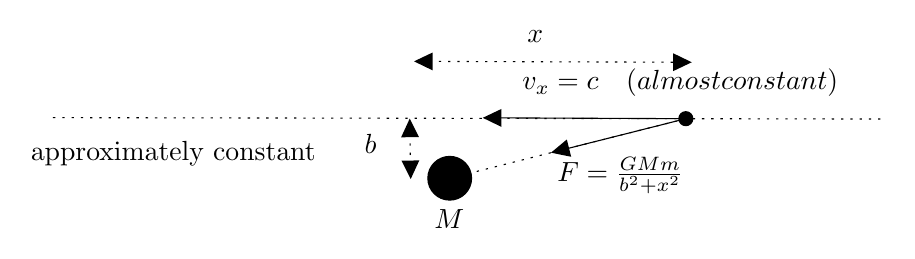
\begin{tikzpicture}[x=0.75pt,y=0.75pt,yscale=-1,xscale=1]
%uncomment if require: \path (0,300); %set diagram left start at 0, and has height of 300

%Shape: Circle [id:dp11215947071202503] 
\draw  [color={rgb, 255:red, 0; green, 0; blue, 0 }  ,draw opacity=1 ][fill={rgb, 255:red, 0; green, 0; blue, 0 }  ,fill opacity=1 ] (285.33,186.6) .. controls (285.33,180.78) and (290.05,176.07) .. (295.87,176.07) .. controls (301.68,176.07) and (306.4,180.78) .. (306.4,186.6) .. controls (306.4,192.42) and (301.68,197.13) .. (295.87,197.13) .. controls (290.05,197.13) and (285.33,192.42) .. (285.33,186.6) -- cycle ;
%Straight Lines [id:da19819751525200946] 
\draw  [dash pattern={on 0.84pt off 2.51pt}]  (104.73,157.4) -- (506.07,158.07) ;
%Shape: Circle [id:dp168965639106339] 
\draw  [fill={rgb, 255:red, 0; green, 0; blue, 0 }  ,fill opacity=1 ] (413,157.9) .. controls (413,156.04) and (411.49,154.53) .. (409.63,154.53) .. controls (407.77,154.53) and (406.27,156.04) .. (406.27,157.9) .. controls (406.27,159.76) and (407.77,161.27) .. (409.63,161.27) .. controls (411.49,161.27) and (413,159.76) .. (413,157.9) -- cycle ;
%Straight Lines [id:da596923484195554] 
\draw  [dash pattern={on 0.84pt off 2.51pt}]  (276.65,160.88) -- (277.02,184) ;
\draw [shift={(277.07,187)}, rotate = 269.08] [fill={rgb, 255:red, 0; green, 0; blue, 0 }  ][line width=0.08]  [draw opacity=0] (8.93,-4.29) -- (0,0) -- (8.93,4.29) -- cycle    ;
\draw [shift={(276.6,157.88)}, rotate = 89.08] [fill={rgb, 255:red, 0; green, 0; blue, 0 }  ][line width=0.08]  [draw opacity=0] (8.93,-4.29) -- (0,0) -- (8.93,4.29) -- cycle    ;
%Straight Lines [id:da6177416030758787] 
\draw    (314.8,157.49) -- (409.63,157.9) ;
\draw [shift={(311.8,157.48)}, rotate = 0.25] [fill={rgb, 255:red, 0; green, 0; blue, 0 }  ][line width=0.08]  [draw opacity=0] (8.93,-4.29) -- (0,0) -- (8.93,4.29) -- cycle    ;
%Straight Lines [id:da8971842810057788] 
\draw  [dash pattern={on 0.84pt off 2.51pt}]  (295.87,186.6) -- (409.63,157.9) ;
%Straight Lines [id:da6203038644998173] 
\draw    (347.59,173.55) -- (409.63,157.9) ;
\draw [shift={(344.68,174.28)}, rotate = 345.85] [fill={rgb, 255:red, 0; green, 0; blue, 0 }  ][line width=0.08]  [draw opacity=0] (8.93,-4.29) -- (0,0) -- (8.93,4.29) -- cycle    ;
%Straight Lines [id:da716098628569452] 
\draw  [dash pattern={on 0.84pt off 2.51pt}]  (281.68,130.29) -- (409.48,130.71) ;
\draw [shift={(412.48,130.72)}, rotate = 180.19] [fill={rgb, 255:red, 0; green, 0; blue, 0 }  ][line width=0.08]  [draw opacity=0] (8.93,-4.29) -- (0,0) -- (8.93,4.29) -- cycle    ;
\draw [shift={(278.68,130.28)}, rotate = 0.19] [fill={rgb, 255:red, 0; green, 0; blue, 0 }  ][line width=0.08]  [draw opacity=0] (8.93,-4.29) -- (0,0) -- (8.93,4.29) -- cycle    ;

% Text Node
\draw (287.2,200.52) node [anchor=north west][inner sep=0.75pt]    {$M$};
% Text Node
\draw (253.6,164.12) node [anchor=north west][inner sep=0.75pt]    {$b$};
% Text Node
\draw (92.8,167.52) node [anchor=north west][inner sep=0.75pt]   [align=left] {approximately constant};
% Text Node
\draw (329.6,132.8) node [anchor=north west][inner sep=0.75pt]    {$v_{x} =c\ \ \ (\text{almost constant)}$};
% Text Node
\draw (346.48,175.32) node [anchor=north west][inner sep=0.75pt]    {$F=\frac{GMm}{b^{2} +x^{2}}$};
% Text Node
\draw (332.08,114.32) node [anchor=north west][inner sep=0.75pt]    {$x$};


\end{tikzpicture}
\end{center}


Net impulse in y-direction, can be calculated as: \\
\[\int_{-\infty}^{\infty} \frac{b}{\sqrt{x^2 + b^2}} \frac{GMm}{x^2 + b^2} dt\]
Here, $x=ct$ 
\[\implies \text{Net impulse in y-direction} = \int_{-\infty}^{\infty} \frac{GMmb}{(c^2 t^2 + b^2)^{3/2}} = \boxed{\frac{2GMm}{bc}}\]

So angle of deviation $\approx \boxed{\frac{2GM}{bc^2}}$ 
\begin{center}
    \tikzset{every picture/.style={line width=0.75pt}} %set default line width to 0.75pt        

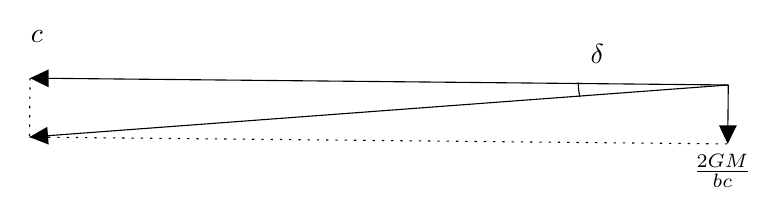
\begin{tikzpicture}[x=0.75pt,y=0.75pt,yscale=-1,xscale=1]
%uncomment if require: \path (0,300); %set diagram left start at 0, and has height of 300

%Straight Lines [id:da23728741683154375] 
\draw    (103,104.03) -- (436.4,107.3) ;
\draw [shift={(100,104)}, rotate = 0.56] [fill={rgb, 255:red, 0; green, 0; blue, 0 }  ][line width=0.08]  [draw opacity=0] (8.93,-4.29) -- (0,0) -- (8.93,4.29) -- cycle    ;
%Straight Lines [id:da3838513843201201] 
\draw    (436.4,107.3) -- (436.16,132.7) ;
\draw [shift={(436.13,135.7)}, rotate = 270.54] [fill={rgb, 255:red, 0; green, 0; blue, 0 }  ][line width=0.08]  [draw opacity=0] (8.93,-4.29) -- (0,0) -- (8.93,4.29) -- cycle    ;
%Straight Lines [id:da9554461222472377] 
\draw  [dash pattern={on 0.84pt off 2.51pt}]  (100,104) -- (99.73,132.4) ;
%Straight Lines [id:da7608816435313206] 
\draw  [dash pattern={on 0.84pt off 2.51pt}]  (99.73,132.4) -- (436.13,135.7) ;
%Straight Lines [id:da016714075583732058] 
\draw    (102.73,132.18) -- (436.4,107.3) ;
\draw [shift={(99.73,132.4)}, rotate = 355.74] [fill={rgb, 255:red, 0; green, 0; blue, 0 }  ][line width=0.08]  [draw opacity=0] (8.93,-4.29) -- (0,0) -- (8.93,4.29) -- cycle    ;
%Shape: Arc [id:dp9084521708514095] 
\draw  [draw opacity=0] (364.91,113.14) .. controls (364.49,111.33) and (364.23,109.45) .. (364.16,107.52) .. controls (364.14,107.02) and (364.13,106.52) .. (364.13,106.02) -- (394.13,106.33) -- cycle ; \draw   (364.91,113.14) .. controls (364.49,111.33) and (364.23,109.45) .. (364.16,107.52) .. controls (364.14,107.02) and (364.13,106.52) .. (364.13,106.02) ;

% Text Node
\draw (368.8,86.2) node [anchor=north west][inner sep=0.75pt]    {$\delta $};
% Text Node
\draw (99.12,79.96) node [anchor=north west][inner sep=0.75pt]    {$c$};
% Text Node
\draw (418.32,139.36) node [anchor=north west][inner sep=0.75pt]    {$\frac{2GM}{bc}$};


\end{tikzpicture}
\end{center}

Now,
\begin{center}
    \tikzset{every picture/.style={line width=0.75pt}} %set default line width to 0.75pt        

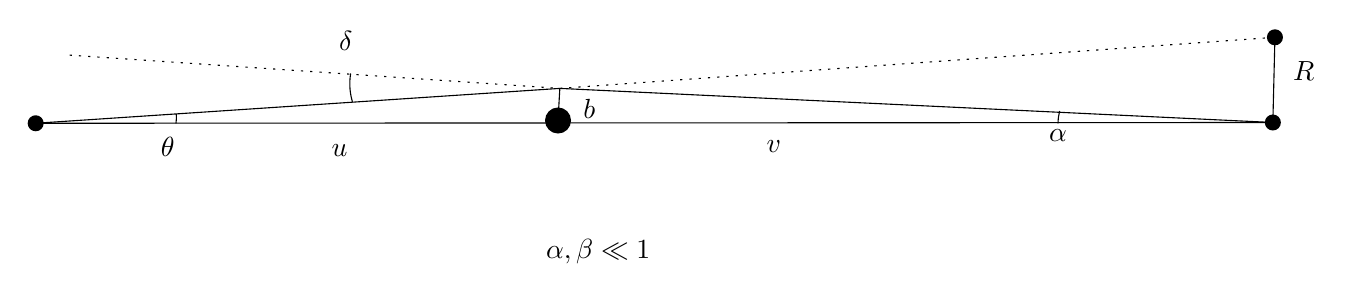
\begin{tikzpicture}[x=0.75pt,y=0.75pt,yscale=-1,xscale=1]
%uncomment if require: \path (0,300); %set diagram left start at 0, and has height of 300

%Straight Lines [id:da8020136276072414] 
\draw    (35.33,191.67) -- (631.4,191.3) ;
\draw [shift={(631.4,191.3)}, rotate = 359.96] [color={rgb, 255:red, 0; green, 0; blue, 0 }  ][fill={rgb, 255:red, 0; green, 0; blue, 0 }  ][line width=0.75]      (0, 0) circle [x radius= 3.35, y radius= 3.35]   ;
\draw [shift={(35.33,191.67)}, rotate = 359.96] [color={rgb, 255:red, 0; green, 0; blue, 0 }  ][fill={rgb, 255:red, 0; green, 0; blue, 0 }  ][line width=0.75]      (0, 0) circle [x radius= 3.35, y radius= 3.35]   ;
%Shape: Circle [id:dp7955971092661203] 
\draw  [fill={rgb, 255:red, 0; green, 0; blue, 0 }  ,fill opacity=1 ] (281,190.34) .. controls (281,187.03) and (283.68,184.34) .. (286.99,184.34) .. controls (290.3,184.34) and (292.99,187.03) .. (292.99,190.34) .. controls (292.99,193.65) and (290.3,196.33) .. (286.99,196.33) .. controls (283.68,196.33) and (281,193.65) .. (281,190.34) -- cycle ;
%Straight Lines [id:da18531049571144775] 
\draw    (35.33,191.67) -- (287.87,174.87) ;
%Straight Lines [id:da33781902485996507] 
\draw    (287.87,174.87) -- (631.4,191.3) ;
%Straight Lines [id:da8500581519465056] 
\draw    (287.87,174.87) -- (286.99,190.34) ;
%Straight Lines [id:da532342163889258] 
\draw  [dash pattern={on 0.84pt off 2.51pt}]  (51.68,158.84) -- (287.87,174.87) ;
%Shape: Arc [id:dp6303850351899705] 
\draw  [draw opacity=0] (187.95,181.33) .. controls (187.38,179.43) and (186.99,177.44) .. (186.8,175.39) .. controls (186.56,172.75) and (186.67,170.16) .. (187.09,167.67) -- (216.68,172.68) -- cycle ; \draw   (187.95,181.33) .. controls (187.38,179.43) and (186.99,177.44) .. (186.8,175.39) .. controls (186.56,172.75) and (186.67,170.16) .. (187.09,167.67) ;
%Straight Lines [id:da09107961058024316] 
\draw  [dash pattern={on 0.84pt off 2.51pt}]  (287.87,174.87) -- (632.4,150.25) ;
%Straight Lines [id:da5066586910759496] 
\draw    (632.4,150.25) -- (631.4,191.3) ;
\draw [shift={(632.4,150.25)}, rotate = 91.4] [color={rgb, 255:red, 0; green, 0; blue, 0 }  ][fill={rgb, 255:red, 0; green, 0; blue, 0 }  ][line width=0.75]      (0, 0) circle [x radius= 3.35, y radius= 3.35]   ;
%Shape: Arc [id:dp08318928063790598] 
\draw  [draw opacity=0] (103.08,187.3) .. controls (103.18,188.79) and (103.13,190.26) .. (102.94,191.71) -- (60.34,190.41) -- cycle ; \draw   (103.08,187.3) .. controls (103.18,188.79) and (103.13,190.26) .. (102.94,191.71) ;
%Shape: Arc [id:dp2619046069077702] 
\draw  [draw opacity=0] (527.9,191.71) .. controls (527.9,189.68) and (528.19,187.7) .. (528.74,185.79) -- (570.75,191.69) -- cycle ; \draw   (527.9,191.71) .. controls (527.9,189.68) and (528.19,187.7) .. (528.74,185.79) ;

% Text Node
\draw (180.28,145.88) node [anchor=north west][inner sep=0.75pt]    {$\delta $};
% Text Node
\draw (297.98,178.88) node [anchor=north west][inner sep=0.75pt]    {$b$};
% Text Node
\draw (176.68,200.68) node [anchor=north west][inner sep=0.75pt]    {$u$};
% Text Node
\draw (386.28,198.68) node [anchor=north west][inner sep=0.75pt]    {$v$};
% Text Node
\draw (639.9,160.7) node [anchor=north west][inner sep=0.75pt]    {$R$};
% Text Node
\draw (94.33,196.99) node [anchor=north west][inner sep=0.75pt]    {$\theta $};
% Text Node
\draw (522.35,193.5) node [anchor=north west][inner sep=0.75pt]    {$\alpha $};
% Text Node
\draw (280,246.4) node [anchor=north west][inner sep=0.75pt]    {$\alpha ,\beta \ll 1$};


\end{tikzpicture}
\end{center}

By exterior angle property, it's clear that \[\delta = \alpha + \theta\] 
\[\implies \frac{2GM}{bc^2} = \frac{b}{u} + \frac{b}{v} \implies b^2 = \frac{2GM}{c^2} \frac{uv}{u+v} = \theta^2 u^2\]
Hence, we can write $\theta$ as \[\theta = \sqrt{\frac{2GMv}{c^2 u (u+v)}}\]

For calculating $R$, we can use basic trigonometry. \\
\[R = (u+v) \tan \theta \approx \theta (v+u)\]
On substituting the value of $\theta$ obtained earlier 
\[R \approx \theta (v+u) = \boxed{\sqrt{\frac{2GMv(u+v)}{uc^2}}}\]

\end{solution}
\vspace{10mm}%\section{Problem 8}

\begin{problem}

A ball of $(R = 10 $m$)$ from height $h=100 m$ on a surface having coefficient of kinetic friction as $\mu_k = 0.5$. After the first collision with the surface, it rebounds (coefficient of restitution = 0.5) and also moves a maximal horizontal distance of $x=1.29 m$. Assuming the ball to be a uniform solid sphere, choose the correct options: \\
(A) It'll slip on the surface for the complete duration of impact. \\
(B) It won't slip for complete duration of impact. \\
(C) Maximum angular velocity being given is $0.1$ rad/s.\\
(D) Maximum angular velocity being given is $0.2$ rad/s.\\


\end{problem}
\begin{flushright}
\textbf{\Large{-Proposed by Atharv Shivram Mahajan}}
\end{flushright}
\begin{solution}
{\Large{\textbf{Answer: BC}}}\\


\begin{center}
    

\tikzset{every picture/.style={line width=0.75pt}} %set default line width to 0.75pt        

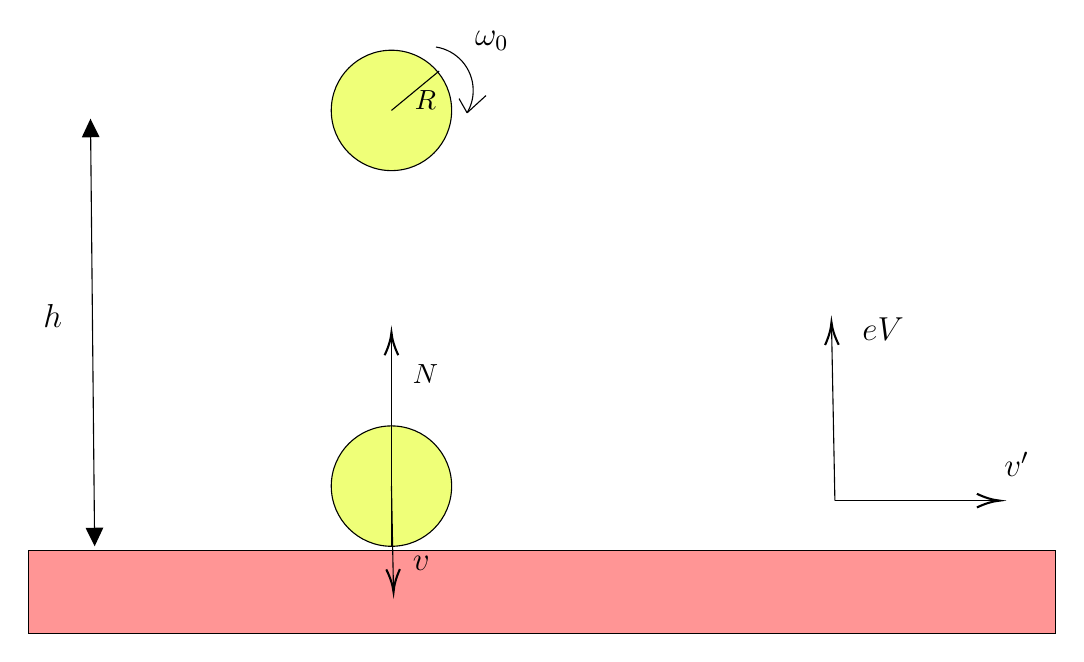
\begin{tikzpicture}[x=0.75pt,y=0.75pt,yscale=-1,xscale=1]
%uncomment if require: \path (0,300); %set diagram left start at 0, and has height of 300

%Shape: Rectangle [id:dp6418623931107614] 
\draw  [fill={rgb, 255:red, 255; green, 149; blue, 149 }  ,fill opacity=1 ] (68,258) -- (563,258) -- (563,298) -- (68,298) -- cycle ;
%Shape: Circle [id:dp9738120739595633] 
\draw  [fill={rgb, 255:red, 239; green, 255; blue, 120 }  ,fill opacity=1 ] (214,227) .. controls (214,210.98) and (226.98,198) .. (243,198) .. controls (259.02,198) and (272,210.98) .. (272,227) .. controls (272,243.02) and (259.02,256) .. (243,256) .. controls (226.98,256) and (214,243.02) .. (214,227) -- cycle ;
%Shape: Circle [id:dp1940159375606385] 
\draw  [fill={rgb, 255:red, 239; green, 255; blue, 120 }  ,fill opacity=1 ] (214,46) .. controls (214,29.98) and (226.98,17) .. (243,17) .. controls (259.02,17) and (272,29.98) .. (272,46) .. controls (272,62.02) and (259.02,75) .. (243,75) .. controls (226.98,75) and (214,62.02) .. (214,46) -- cycle ;
%Straight Lines [id:da6905653335773223] 
\draw    (243,46) -- (266,27) ;
%Shape: Arc [id:dp10080055131687193] 
\draw  [draw opacity=0] (264.47,15.46) .. controls (274.47,17.01) and (282.2,25.57) .. (282.38,36.03) .. controls (282.45,40.09) and (281.37,43.89) .. (279.45,47.15) -- (261.21,36.39) -- cycle ; \draw   (264.47,15.46) .. controls (274.47,17.01) and (282.2,25.57) .. (282.38,36.03) .. controls (282.45,40.09) and (281.37,43.89) .. (279.45,47.15) ;
%Straight Lines [id:da3659285013611038] 
\draw    (288.52,38.87) -- (279.45,47.15) ;
%Straight Lines [id:da48359158620569964] 
\draw    (275.56,40.31) -- (279.45,47.15) ;

%Straight Lines [id:da7858703833224256] 
\draw    (243,227) -- (243.96,276) ;
\draw [shift={(244,278)}, rotate = 268.88] [color={rgb, 255:red, 0; green, 0; blue, 0 }  ][line width=0.75]    (10.93,-3.29) .. controls (6.95,-1.4) and (3.31,-0.3) .. (0,0) .. controls (3.31,0.3) and (6.95,1.4) .. (10.93,3.29)   ;
%Straight Lines [id:da6003288604165082] 
\draw    (243,256) -- (243,155) ;
\draw [shift={(243,153)}, rotate = 450] [color={rgb, 255:red, 0; green, 0; blue, 0 }  ][line width=0.75]    (10.93,-3.29) .. controls (6.95,-1.4) and (3.31,-0.3) .. (0,0) .. controls (3.31,0.3) and (6.95,1.4) .. (10.93,3.29)   ;
%Straight Lines [id:da3654706704551074] 
\draw    (98.03,53) -- (99.97,253) ;
\draw [shift={(100,256)}, rotate = 269.44] [fill={rgb, 255:red, 0; green, 0; blue, 0 }  ][line width=0.08]  [draw opacity=0] (8.93,-4.29) -- (0,0) -- (8.93,4.29) -- cycle    ;
\draw [shift={(98,50)}, rotate = 89.44] [fill={rgb, 255:red, 0; green, 0; blue, 0 }  ][line width=0.08]  [draw opacity=0] (8.93,-4.29) -- (0,0) -- (8.93,4.29) -- cycle    ;
%Straight Lines [id:da7417223204793537] 
\draw    (456.65,234) -- (455.04,150.04) ;
\draw [shift={(455,148.04)}, rotate = 448.9] [color={rgb, 255:red, 0; green, 0; blue, 0 }  ][line width=0.75]    (10.93,-3.29) .. controls (6.95,-1.4) and (3.31,-0.3) .. (0,0) .. controls (3.31,0.3) and (6.95,1.4) .. (10.93,3.29)   ;
%Straight Lines [id:da9320121111232484] 
\draw    (456.65,234) -- (534,234) ;
\draw [shift={(536,234)}, rotate = 180] [color={rgb, 255:red, 0; green, 0; blue, 0 }  ][line width=0.75]    (10.93,-3.29) .. controls (6.95,-1.4) and (3.31,-0.3) .. (0,0) .. controls (3.31,0.3) and (6.95,1.4) .. (10.93,3.29)   ;


% Text Node
\draw (253,35.4) node [anchor=north west][inner sep=0.75pt]    {$R$};
% Text Node
\draw (282,6.4) node [anchor=north west][inner sep=0.75pt]  [font=\large]  {$\omega _{0}$};
% Text Node
\draw (252,259.4) node [anchor=north west][inner sep=0.75pt]  [font=\large]  {$v$};
% Text Node
\draw (252,167.4) node [anchor=north west][inner sep=0.75pt]    {$N$};
% Text Node
\draw (74,138.4) node [anchor=north west][inner sep=0.75pt]  [font=\large]  {$h$};
% Text Node
\draw (462,142.4) node [anchor=north west][inner sep=0.75pt]  [font=\large]  {$ \begin{array}{l}
eV\\
\end{array}$};
% Text Node
\draw (537,209.4) node [anchor=north west][inner sep=0.75pt]  [font=\large]  {$v'$};

\end{tikzpicture}
\end{center}


$$\int Ndt = mv(1+e)$$
Now first lets say it slips for all the time during collision.
$$\mu \int Ndt = mv'$$
$\implies$Time of flight before $2nd$ collision = $\frac{2eV}{g}$\\
$\implies$Range = $x$ = $\frac{mu \int Ndt}{m}.\frac{2eV}{g}$\\
On substituting with values and simplifying, we get: $x  = 100m$
but $x=1.29m$ is given.\\
Hence, it can't slip for all the time.
$$\therefore \mu.R.\int_{0}^{t} Ndt = I\left(\omega_0 - \frac{v'}{R}\right)$$
$$ \text{and} \mu \int_{0}^{t}N.dt = mv'$$
Using these two equations, we get:
$$R = \frac{I}{mv'}\left(\omega_0 - \frac{v'}{R}\right)$$
So,
$$\omega_0 = v' \left(\frac{mR^2}{IR}+\frac{1}{R}\right)$$
$$\omega_0 = \frac{7v'}{2R}$$
Also:
$$v' = \frac{xg}{2eV} = \frac{1.29 \times g}{\sqrt{2gh}}$$
Using this we get:
$$\boxed{\omega = 0.1 rad/s}$$


\end{solution}
\vspace{10mm}%\section{Problem 9}
\begin{problem}

\begin{center}
    \textbf{Photon gas on a carnot engine ride}
\end{center}
\vspace{5mm}


\begin{center}
    

% Pattern Info
 
\tikzset{
pattern size/.store in=\mcSize, 
pattern size = 5pt,
pattern thickness/.store in=\mcThickness, 
pattern thickness = 0.3pt,
pattern radius/.store in=\mcRadius, 
pattern radius = 1pt}
\makeatletter
\pgfutil@ifundefined{pgf@pattern@name@_1dl0yf2qx}{
\pgfdeclarepatternformonly[\mcThickness,\mcSize]{_1dl0yf2qx}
{\pgfqpoint{0pt}{0pt}}
{\pgfpoint{\mcSize+\mcThickness}{\mcSize+\mcThickness}}
{\pgfpoint{\mcSize}{\mcSize}}
{
\pgfsetcolor{\tikz@pattern@color}
\pgfsetlinewidth{\mcThickness}
\pgfpathmoveto{\pgfqpoint{0pt}{0pt}}
\pgfpathlineto{\pgfpoint{\mcSize+\mcThickness}{\mcSize+\mcThickness}}
\pgfusepath{stroke}
}}
\makeatother
\tikzset{every picture/.style={line width=0.75pt}} %set default line width to 0.75pt        

\begin{tikzpicture}[x=0.75pt,y=0.75pt,yscale=-1,xscale=1]
\path (0,456); %set diagram left start at 0, and has height of 456

%Shape: Rectangle [id:dp9834446001190817] 
\draw  [color={rgb, 255:red, 128; green, 120; blue, 121 }  ,draw opacity=1 ][pattern=_1dl0yf2qx,pattern size=6pt,pattern thickness=0.75pt,pattern radius=0pt, pattern color={rgb, 255:red, 68; green, 93; blue, 122}] (209,121.5) -- (234,121.5) -- (234,246.5) -- (209,246.5) -- cycle ;
%Straight Lines [id:da753188734556363] 
\draw [color={rgb, 255:red, 49; green, 49; blue, 49 }  ,draw opacity=0.67 ][line width=3]    (100,122) -- (420,122) ;
%Straight Lines [id:da8085392531859608] 
\draw [color={rgb, 255:red, 49; green, 49; blue, 49 }  ,draw opacity=0.67 ][line width=3]    (100,246.5) -- (421,246.5) ;
%Straight Lines [id:da2496628708265749] 
\draw [color={rgb, 255:red, 49; green, 49; blue, 49 }  ,draw opacity=0.67 ][line width=3]    (100,248.5) -- (100,120) ;
%Straight Lines [id:da8684195869872635] 
\draw [line width=1.5]    (212,45) -- (171.95,116.51) ;
\draw [shift={(170,120)}, rotate = 299.25] [fill={rgb, 255:red, 0; green, 0; blue, 0 }  ][line width=0.08]  [draw opacity=0] (18.57,-8.92) -- (0,0) -- (18.57,8.92) -- cycle    ;

% Text Node
\draw (145,167.4) node [anchor=north west][inner sep=0.75pt]  [font=\LARGE]  {$V$};
% Text Node
\draw (185,18.4) node [anchor=north west][inner sep=0.75pt]  [font=\LARGE]  {$T$};


\end{tikzpicture}

\end{center}
\vspace{5mm}

A container with a piston shown in the figure, has a photon gas characterised by state equations of Internal energy $U(T,V)$ and pressure $P(T)$ which are 
\[U(T,V) = b V T^4\] 
\[P(T) = \frac{1}{3} bT^4\]
where $b$ is a dimensioned constant, $V$ is the volume of system, T is its temperature. \\
Let's take the gas through a carnot cycle, starting with $V=0$ and temperature of the enclosure $T_H$ and sequentially take it through \\
\textbf{Process 1} : Isothermal expansion at temperature $T_H$ to a volume $V_1$. \\
\textbf{Process 2} : Adiabatic expansion to a volume $V_2$. \\
\textbf{Process 3} : Isothermal compression to zero volume at temperature $T_c$.\\
\textbf{Process 4} : Heating back the enclosure from $T_c$ to $T_H$ at zero volume. \\

Mark the correct option(s): \\
(a) The enclosure acts as perfect reflector for photons during process-2.\\
(b) The change in entropy of the photon gas during process 3 is $- \frac{1}{3} b T_{c}^{3} V_2$ . \\
(c) The process equation for process-2 is $PV^{4/3}=$ constant. \\
(d) Ratio of number of photons in the enclosure at same volume $\frac{V_1}{2}$ but during process-1 to process-3 is $\frac{T_{H}^{4}}{T_{C}^{4}}$.



\end{problem}
\begin{flushright}
\textbf{\Large{-Proposed by Janardanudu Thallaparthi}}
\end{flushright}
\begin{solution}
{\Large{\textbf{Answer: AC}}}\\
\
Process 1-3 is isothermal\
\
$$U=bVT^4 \rightarrow dU=bT^4dV=3PdV$$
$$P=\frac{b}{3}T^4 \rightarrow dQ=dU+dW=4PdV$$
So, $W=\frac{1}{3}bT^4\Delta V$ and $Q=\frac{4}{3}bT^4\Delta V$
Also, $S=\frac{4}{3}bVT^3$ so option $B$ is wrong.\
\rule{\textwidth}{0.4pt}
For process $2$, which is adiabatic
``$S$'' should not change $\rightarrow VT^3 = \text{constant}$
$\rightarrow PV^{\frac{4}{3}}=$constant, also number of photons remain constant as walls cannot emit or absorb photons during adiabatic process. So walls are considered perfect reflectors in process $2$

\rule{\textwidth}{0.4pt}
Also, in adiabatic process, Number of photons $N$ and entropy $S$ are constant
$$\rightarrow N=\alpha S, \text{Where} N \ \text{is a constant}$$
$$\rightarrow \frac{N_1}{N_2}=\frac{S_1}{S_2}=\frac{\frac{4}{3}b V_1 T^3_1 }{{4 \over 3}bV_2 T_2^3}=\frac{T_1^3}{T_2^3}\ \text{as same volume}$$

\end{solution}
\vspace{10mm}%\section{Problem 10}


\begin{problem}

A sphere of radius $r_1=1m$ is placed concentrically in a thin shell of radius $r_2=3m$ with emmisivities $e_1$ and $e_2$ respectively. The inner sphere generates a constant power $P$. Assume that none of the surfaces allow transmission. Also assume that space between sphere and outer shell is a vacuum.T is steady state temperature of inner sphere.Then Choose the correct option(s):\

A.If $e_1=0.30$ and $e_2=0.50$, \hspace{0.3cm}$11P=12\sigma\pi{T}^4$ \\

B.If $e_1=0.30$ and $e_2=0.50$,\hspace{0.3cm}$91P=3\sigma\pi{T}^4$ \\

C.If $e_1=0.20$ and $e_2=0.40$,\hspace{0.3cm} $49P=36 \sigma\pi{T}^4$ \\

D.If $e_1=0.20$ and $e_2=0.40$,\hspace{0.3cm} $92P=3\sigma\pi{T}^4$ \\

\begin{center}

 \includegraphics[width=0.6\textwidth]{akiii.png}
\end{center}

\end{problem}
\begin{flushright}
\textbf{\Large{-Proposed by AKIII}}
\end{flushright}
\begin{solution}

{\Large{\textbf{Answer: (A), (C)}}}\\

\Large{\textbf{Solution-1:}}\\

\begin{center}
    

\tikzset{every picture/.style={line width=0.75pt}} %set default line width to 0.75pt        

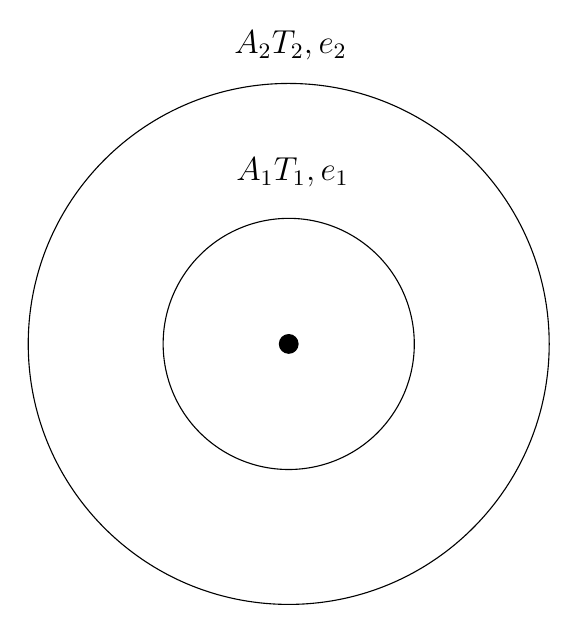
\begin{tikzpicture}[x=0.75pt,y=0.75pt,yscale=-1,xscale=1]
%uncomment if require: \path (0,750); %set diagram left start at 0, and has height of 750

%Shape: Circle [id:dp43510073183542763] 
\draw   (198,160.5) .. controls (198,91.19) and (254.19,35) .. (323.5,35) .. controls (392.81,35) and (449,91.19) .. (449,160.5) .. controls (449,229.81) and (392.81,286) .. (323.5,286) .. controls (254.19,286) and (198,229.81) .. (198,160.5) -- cycle ;
%Shape: Circle [id:dp40706058127534406] 
\draw   (273.95,125.79) .. controls (293.12,98.42) and (330.84,91.78) .. (358.21,110.95) .. controls (385.58,130.12) and (392.22,167.84) .. (373.05,195.21) .. controls (353.88,222.58) and (316.16,229.22) .. (288.79,210.05) .. controls (261.42,190.88) and (254.78,153.16) .. (273.95,125.79) -- cycle ;
%Shape: Circle [id:dp05272636104833883] 
\draw  [fill={rgb, 255:red, 0; green, 0; blue, 0 }  ,fill opacity=1 ] (319,160.5) .. controls (319,158.01) and (321.01,156) .. (323.5,156) .. controls (325.99,156) and (328,158.01) .. (328,160.5) .. controls (328,162.99) and (325.99,165) .. (323.5,165) .. controls (321.01,165) and (319,162.99) .. (319,160.5) -- cycle ;

% Text Node
\draw (297,69.4) node [anchor=north west][inner sep=0.75pt]  [font=\large]  {$A_{1} T_{1} ,e_{1}$};
% Text Node
\draw (296,8.4) node [anchor=north west][inner sep=0.75pt]  [font=\large]  {$A_{2} T_{2} ,e_{2}$};


\end{tikzpicture}

\end{center}
\normalsize{As seen from outside, net power} $P$ should be coming out.
Let $ T$ be the steady state temperature of the inner shell and $T_2$ be the steady state temperature of the outer shell.\\
$$\therefore \sigma e_2 A_2 T_{2}^4 = P$$
Let total power absorbed by the outer shell be = $k$.\\
For steady state of the outer shell:\\
$$k = 2\sigma e_2 A_2 T_{2}^4 $$
$$k=2P$$
If the outer shell absorbs power, then it must have received $\frac{k}{e_2}$ power.\\
The radiations that outer shell receives are from some of its own radiations that fall on itself, coming from the inner sphere.\\
$\therefore$It has reflected $\frac{k}{e_2}(1-e_2)$ Power.\\
\\
Out of this, \\
$\frac{k}{e_2}(1-e_2). \frac{A_1}{A_2}e_1$ is absorbed by the inner shell.\\
\\
So, for the inner shell:
$$P\frac{k}{e_2}(1-e_2). \frac{A_1}{A_2}e_1+P \frac{A_1}{A_2} e_1 = \sigma A_1 e_1 T^4$$
( $P\frac{A_1}{A_2} e_1$ is the direct radiation from the outer shell. )
$$\sigma A_1 e_1 T^4= P \frac{A_1}{A_2} e_1 \frac{2-e_2}{e_2} + P$$
$$\boxed{\sigma A_1 e_1 T^4= P \left(\frac{A_1}{A_2} e_1 \frac{2-e_2}{e_2}+1\right)}$$
\Large{\textbf{Solution-2:}}\\
\normalsize{$X$=Power falling on inner sphere}\\
$Y$=Power coming out of the inner sphere(radiated+reflected)\\
$$\implies Y-X = \sigma$$
$$Y = X(1-e_1) + e_1 A_1 \sigma T^4$$
where:\\
$X(1-e_1)$ is the reflected part and $e_1 A_1 \sigma T^4$ is the radiated part.\\
Considering the equation of the outer shell:
\begin{equation*}\label{1}
P\left(\frac{A_1}{A_2}\right)+P\left(\left(1-\frac{A_1}{A_2}\right)(1-e_2)\frac{A_1}{A_2} \cdots \right) + P =Ye_2 + Y(1-e_2) \left(1- \frac{A_1}{A_2}e_2+\cdots \right)
\end{equation*}
$$Ye_2 = P \left(2\frac{A_1}{A_2} + e_2 - \frac{A_1}{A_2}e_2\right)$$
$$Y = P \left(\frac{A_1}{A_2}\left(\frac{2-e_1}{e_2}\right)+1\right)$$
Also,
$$Ye_1 + P(1-e_1) = e_1 A_1 \sigma T^4$$
So,
$$P\left(\frac{A_1}{A_2} \left(\frac{2-e_2}{e_2}\right)e_1 + e_1 + 1 - e_1\right) = e_1 A_1 \sigma T^4$$
$$\boxed{\sigma A_1 e_1 T^4= P \left(\frac{A_1}{A_2} e_1 \frac{2-e_2}{e_2}+1\right)}$$
$\therefore$ Energy flow from the inner sphere to the outer sphere is not considered in $X$ and $Y$, we must account it separately in (\ref{1}).
\end{solution}
\vspace{10mm}%\section{Problem 11}
\begin{problem}

Consider the region $y\ge 0$ in the cartesian plane filled by a certain material whose refractive index  is a function of the vertical distance ($y$) from the $x$ axis.
\begin{equation*}
n(y)=ay \hspace{1cm} (y>0)
\end{equation*}
Where $n(0)=n_0$ and $a$ is a constant with dimension $[L]^{-1}$
A ray of light is incident to this region at the origin making an angle $\theta_0$ with the vertical.
If 
$$y(x)=K\frac{n_0\sin\theta_0
[\exp{(2ax)/(n_0\sin\theta_0)}+1]}{a\exp[(ax)/(n_0\sin\theta_0)]}$$
Report the value of $(2K+1)^{(2K+1)}$ as the answer.
If the setup is impossible, enter 0
\end{problem}
\begin{flushright}
\textbf{\Large{-Proposed by Muhammed Yaseen Nivas}}
\end{flushright}
\begin{solution}
{\Large{\textbf{Answer: 0}}}\\
As we can see $n(0)=n_0$, but $n(0^{+})\to 0$. So, Total internal refraction occurs and the setup is impossible, hence answer is 0.

But in case we assume the ray passes through to the second medium, this is how we solve it:





The angle $\theta$, that the tangent to the graph of a function $y(x)$ makes with the $y$ axis clearly satisfies
$$\tan\theta=\frac{1}{y'(x)}$$
Trigonometric manipulations leads us to 
$$\sin\theta=\frac{1}{\sqrt{1+(y')^2}}$$
Now, coming to physics; to solve this problem, we use Snell's law to write that
\begin{equation*}
    n(y)\sin\theta=c
\end{equation*}
Where $c$ is determined by the initial conditions $n(0)=n_0$, $\theta(y)=\theta_0$. Plugging them in,
$$\frac{ay}{\sqrt{1+(y')^2}}=c\iff\sqrt{\frac{a^2y^2-c^2}{c^2
}}=\dv{y}{x}$$
$$\int_0^x\frac{a\dd x}{c}=\int_0^{y}\frac{\dd y}{\sqrt{y^2-c^2/a^2}}$$

$$\frac{ax}{c}=\frac{1}{2}\ln\left|\frac{\sqrt{y^2-c^2/a^2}+y}{\sqrt{y^2-c^2/a^2}-y}\right|$$
Two cases, either the argument of the logarithm is positive, in which case we can drop the absolute values. We will consider this first.
$$\exp\left(\frac{2ax}{c}\right)=\frac{\sqrt{y^2-c^2/a^2}+y}{\sqrt{y^2-c^2/a^2}-y}$$
$$\exp\left(\frac{2ax}{c}\right)(\sqrt{y^2-c^2/a^2}-y)=\sqrt{y^2-c^2/a^2}+y$$
$$(\sqrt{y^2-c^2/a^2})(\exp(2ax/c)-1)=y(\exp(2ax/c)+1)$$
$$y^2-c^2/a^2=y^2\alpha^2$$
Where, $$\alpha(x)\equiv\frac{\exp(2ax/c)+1}{\exp(2ax/c)-1}$$
$$y^2(1-\alpha^2)=c^2/a^2$$
$$y=\frac{c}{a}\sqrt{\frac{1}{1-\alpha^2}}$$

\begin{equation*}
    \boxed{y(x)=\frac{n_0\sin\theta_0}{a}\sqrt{\frac{1}{1-\alpha^2}}}
\end{equation*}
This function is undefined, so we have to consider the other case.
$$\exp\left(\frac{2ax}{c}\right)=\frac{\sqrt{y^2-c^2/a^2}+y}{-\sqrt{y^2-c^2/a^2}+y}$$
$$\exp\left(\frac{2ax}{c}\right)(y-\sqrt{y^2-c^2/a^2})=\sqrt{y^2-c^2/a^2}+y$$
$$y(\exp\left(\frac{2ax}{c}\right)-1)=\sqrt{y^2-c^2/a^2}(\exp\left(\frac{2ax}{c}\right)+1)$$
$$y^2\beta^2=y^2-c^2/a^2$$
$$y^2(1-\beta^2)=c^2/a^2$$
Where $\beta=\frac{\exp(2ax/c)-1}{\exp(2ax/c+1)}$.
$$y=\frac{c}{a}\sqrt{\frac{1}{1-(\frac{\exp(2ax/c)-1}{\exp(2ax/c)+1})^2}}$$
$$y=\frac{c}{a}\sqrt{\frac{(\exp(2ax/c)+1)^2}{(\exp(2ax/c)+1)^2-(\exp(2ax/c)-1)^2}}$$
$$y=\frac{c}{a}\sqrt{\frac{(\exp(2ax/c)+1)^2}{4\exp(2ax/c)}}$$

$$y=\frac{n_0\sin\theta_0
(\exp(2ax/n_0\sin\theta_0)+1)}{2a\exp(ax/n_0\sin\theta_0)}$$

So in case we did assume ray to pass through this would be the trajectory equation.
\end{solution}
\vspace{10mm}%\section{Problem 12}

\begin{problem}

A cube of side $2a$ and specific gravity $s$ floats in a calm water. "Water line section" is the cross-section of cube intersecting free surface of water. \\
If the cube is given a small angular displacement about centre of water line section and released then, 

%TikZ should be added wrapping the text here. 
\begin{center}
    

\tikzset{every picture/.style={line width=0.75pt}} %set default line width to 0.75pt        

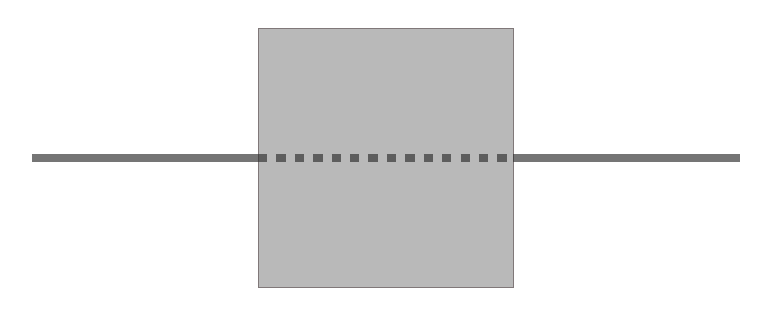
\begin{tikzpicture}[x=0.75pt,y=0.75pt,yscale=-1,xscale=1]
%uncomment if require: \path (0,456); %set diagram left start at 0, and has height of 456

%Shape: Rectangle [id:dp9834446001190817] 
\draw  [color={rgb, 255:red, 128; green, 120; blue, 121 }  ,draw opacity=1 ][fill={rgb, 255:red, 185; green, 185; blue, 185 }  ,fill opacity=1 ] (209,59.5) -- (332,59.5) -- (332,184.5) -- (209,184.5) -- cycle ;
%Straight Lines [id:da753188734556363] 
\draw [color={rgb, 255:red, 49; green, 49; blue, 49 }  ,draw opacity=0.67 ][line width=3]    (100,122) -- (209,122) ;
%Straight Lines [id:da8085392531859608] 
\draw [color={rgb, 255:red, 49; green, 49; blue, 49 }  ,draw opacity=0.67 ][line width=3]    (332,122) -- (441,122) ;
%Straight Lines [id:da6696611451756358] 
\draw [color={rgb, 255:red, 49; green, 49; blue, 49 }  ,draw opacity=0.67 ][line width=3]  [dash pattern={on 3.38pt off 3.27pt}]  (209,122) -- (332,122) ;




\end{tikzpicture}

\end{center}

(a) Volume of cube submerged is increased due to small angular displacement. \\
(b) Volume of the cube submerged remains same even after small angular displacement.\\
(c) For the stability of rotational equilibrium of cube, the condition required is $4s^2 - 4s + 1 >0$ \\
(d) For the stability of rotational equilibrium of cube, the condition required is $6s^2 - 6s + 1 >0$

\end{problem}
\begin{flushright}
\textbf{\Large{-Proposed by Janardanudu Thallaparthi}}
\end{flushright}
\begin{solution}
{\Large{\textbf{Answer: BD}}}\\
Volume submerged remains same for any arbitrary shaped water line cross section. Top view of this section is shown here: \\
\begin{center}
    \tikzset{every picture/.style={line width=0.75pt}} %set default line width to 0.75pt        

\begin{tikzpicture}[x=0.75pt,y=0.75pt,yscale=-1,xscale=1]
%uncomment if require: \path (0,300); %set diagram left start at 0, and has height of 300

%Shape: Polygon Curved [id:ds43972774673161075] 
\draw   (317.8,54.2) .. controls (333.3,59.89) and (372.01,41.71) .. (393.8,44.2) .. controls (415.59,46.69) and (408.89,69.53) .. (426.8,78.2) .. controls (444.71,86.87) and (465.55,81.88) .. (476.8,96.2) .. controls (488.05,110.52) and (459.28,140.33) .. (460.8,147.2) .. controls (462.32,154.07) and (470.84,172.34) .. (425.8,181.2) .. controls (380.76,190.06) and (394.41,189.72) .. (386.8,190.2) .. controls (379.19,190.68) and (372.65,208.23) .. (351.8,199.2) .. controls (330.95,190.17) and (316.8,193.2) .. (305.8,204.2) .. controls (294.8,215.2) and (284.83,191.3) .. (267.8,189.2) .. controls (250.77,187.1) and (243.05,185.39) .. (227.8,188.2) .. controls (212.55,191.01) and (201.2,187.09) .. (188.8,186.2) .. controls (176.4,185.31) and (167.51,170.25) .. (158.27,166.52) .. controls (149.02,162.79) and (143.87,143.66) .. (151.8,132.2) .. controls (159.73,120.74) and (168.06,116.81) .. (173.8,106.2) .. controls (179.54,95.59) and (177.94,86.61) .. (181.8,75.2) .. controls (185.66,63.79) and (198.93,59.23) .. (210.8,53.2) .. controls (222.67,47.17) and (247.79,62.05) .. (263.8,60.2) .. controls (279.81,58.35) and (302.3,48.51) .. (317.8,54.2) -- cycle ;
%Straight Lines [id:da6479538482849021] 
\draw  [dash pattern={on 4.5pt off 4.5pt}]  (303.3,17.7) -- (303.3,229.7) ;
%Shape: Circle [id:dp12930477765964143] 
\draw  [fill={rgb, 255:red, 0; green, 0; blue, 0 }  ,fill opacity=1 ] (305.8,126.2) .. controls (305.8,124.82) and (304.68,123.7) .. (303.3,123.7) .. controls (301.92,123.7) and (300.8,124.82) .. (300.8,126.2) .. controls (300.8,127.58) and (301.92,128.7) .. (303.3,128.7) .. controls (304.68,128.7) and (305.8,127.58) .. (305.8,126.2) -- cycle ;
%Straight Lines [id:da9954861417078642] 
\draw [color={rgb, 255:red, 208; green, 2; blue, 27 }  ,draw opacity=1 ]   (301.3,217.69) -- (221.8,217.21) ;
\draw [shift={(219.8,217.2)}, rotate = 360.34000000000003] [color={rgb, 255:red, 208; green, 2; blue, 27 }  ,draw opacity=1 ][line width=0.75]    (10.93,-3.29) .. controls (6.95,-1.4) and (3.31,-0.3) .. (0,0) .. controls (3.31,0.3) and (6.95,1.4) .. (10.93,3.29)   ;
\draw [shift={(303.3,217.7)}, rotate = 180.34] [color={rgb, 255:red, 208; green, 2; blue, 27 }  ,draw opacity=1 ][line width=0.75]    (10.93,-3.29) .. controls (6.95,-1.4) and (3.31,-0.3) .. (0,0) .. controls (3.31,0.3) and (6.95,1.4) .. (10.93,3.29)   ;
%Straight Lines [id:da8891529338241608] 
\draw [color={rgb, 255:red, 208; green, 2; blue, 27 }  ,draw opacity=1 ]   (403.8,218.19) -- (305.3,217.71) ;
\draw [shift={(303.3,217.7)}, rotate = 360.28] [color={rgb, 255:red, 208; green, 2; blue, 27 }  ,draw opacity=1 ][line width=0.75]    (10.93,-3.29) .. controls (6.95,-1.4) and (3.31,-0.3) .. (0,0) .. controls (3.31,0.3) and (6.95,1.4) .. (10.93,3.29)   ;
\draw [shift={(405.8,218.2)}, rotate = 180.28] [color={rgb, 255:red, 208; green, 2; blue, 27 }  ,draw opacity=1 ][line width=0.75]    (10.93,-3.29) .. controls (6.95,-1.4) and (3.31,-0.3) .. (0,0) .. controls (3.31,0.3) and (6.95,1.4) .. (10.93,3.29)   ;

% Text Node
\draw (307,112.4) node [anchor=north west][inner sep=0.75pt]  [font=\small,color={rgb, 255:red, 74; green, 144; blue, 226 }  ,opacity=1 ]  {$\mathbf{G}$};
% Text Node
\draw (212,109.4) node [anchor=north west][inner sep=0.75pt]  [color={rgb, 255:red, 74; green, 144; blue, 226 }  ,opacity=1 ]  {$\mathbf{G_{1}}$};
% Text Node
\draw (389,105.4) node [anchor=north west][inner sep=0.75pt]  [color={rgb, 255:red, 74; green, 144; blue, 226 }  ,opacity=1 ]  {$\mathbf{G_{2}}$};
% Text Node
\draw (249,218.4) node [anchor=north west][inner sep=0.75pt]    {$x_{1}$};
% Text Node
\draw (344,218.4) node [anchor=north west][inner sep=0.75pt]    {$x_{2}$};


\end{tikzpicture}
\end{center}

For small angular displacements, $G_1G$  moves up by $x_1,\theta$ and $GG_2$ moves down by $x_2 \theta$, For equilibrium initially $A_1 x_1 = A_2 x_2$ where $A_1$ and $A_2$ are areas left and right of dashed horizontal line.
So, $A_1 x_1 \theta = A_2 x_2 \theta$ represents equal volumes by Pappus' theorem. Hence, volume submerged remains unchanged. So, buoyant forces remains unchanged. 

Let's first establish an important point. \\

\begin{center}
    \tikzset{every picture/.style={line width=0.75pt}} %set default line width to 0.75pt        

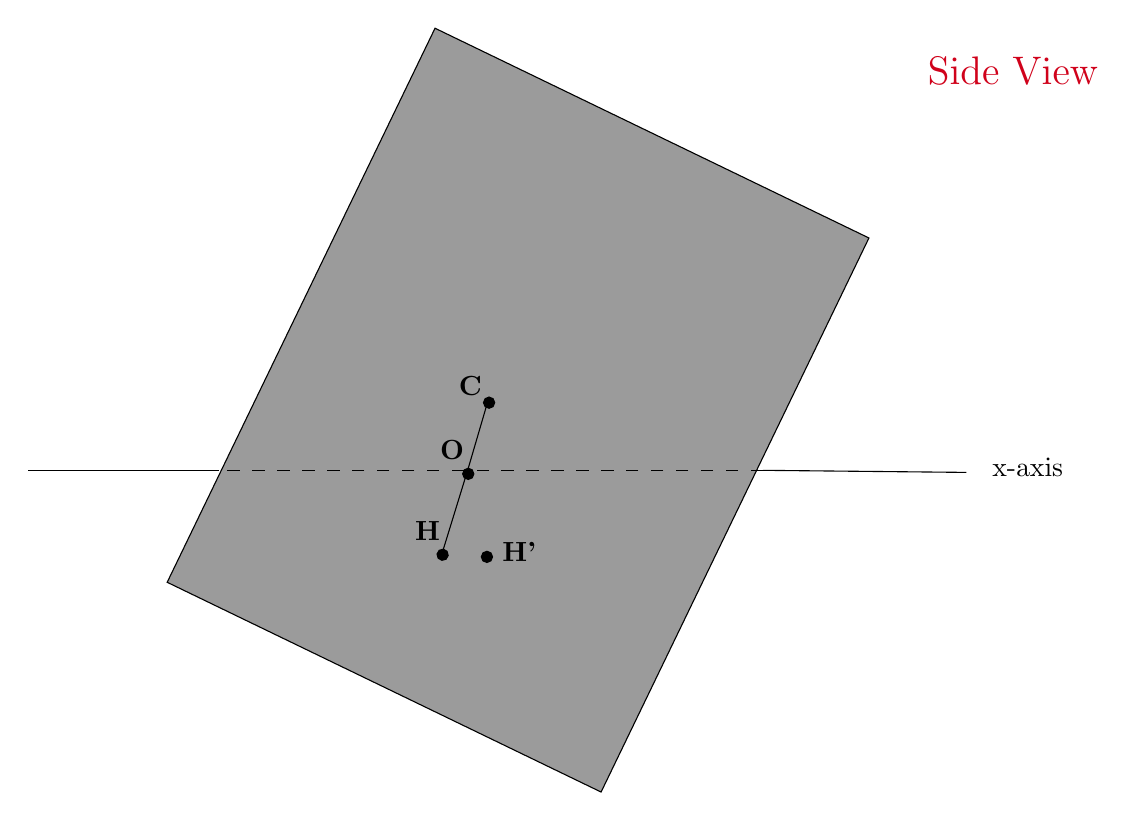
\begin{tikzpicture}[x=0.75pt,y=0.75pt,yscale=-1,xscale=1]
%uncomment if require: \path (0,413); %set diagram left start at 0, and has height of 413

%Shape: Rectangle [id:dp30156020672306183] 
\draw  [fill={rgb, 255:red, 155; green, 155; blue, 155 }  ,fill opacity=1 ] (297.8,9.4) -- (506.85,110.46) -- (377.8,377.4) -- (168.75,276.34) -- cycle ;
%Straight Lines [id:da7592983181523243] 
\draw    (101.8,222.4) -- (193.8,222.4) ;
%Straight Lines [id:da5791562889977035] 
\draw  [dash pattern={on 4.5pt off 4.5pt}]  (455.8,222.4) -- (193.8,222.4) ;
%Straight Lines [id:da9498094883394255] 
\draw    (455.8,222.4) -- (553.8,223.4) ;
%Straight Lines [id:da6773445467137911] 
\draw    (313.8,221.4) -- (301.8,260.4) ;
%Shape: Boxed Line [id:dp9563402454815142] 
\draw    (313.8,221.4) -- (323.84,187.1) ;
%Shape: Circle [id:dp04930614907590947] 
\draw  [fill={rgb, 255:red, 0; green, 0; blue, 0 }  ,fill opacity=1 ] (311.1,224.1) .. controls (311.1,222.61) and (312.31,221.4) .. (313.8,221.4) .. controls (315.29,221.4) and (316.5,222.61) .. (316.5,224.1) .. controls (316.5,225.59) and (315.29,226.8) .. (313.8,226.8) .. controls (312.31,226.8) and (311.1,225.59) .. (311.1,224.1) -- cycle ;
%Shape: Circle [id:dp6118305402832833] 
\draw  [fill={rgb, 255:red, 0; green, 0; blue, 0 }  ,fill opacity=1 ] (298.77,262.73) .. controls (298.97,261.25) and (300.32,260.21) .. (301.8,260.4) .. controls (303.28,260.59) and (304.32,261.95) .. (304.13,263.43) .. controls (303.94,264.9) and (302.58,265.95) .. (301.1,265.76) .. controls (299.63,265.56) and (298.58,264.21) .. (298.77,262.73) -- cycle ;
%Shape: Circle [id:dp38935218699000407] 
\draw  [fill={rgb, 255:red, 0; green, 0; blue, 0 }  ,fill opacity=1 ] (321.14,189.8) .. controls (321.14,188.31) and (322.35,187.1) .. (323.84,187.1) .. controls (325.33,187.1) and (326.54,188.31) .. (326.54,189.8) .. controls (326.54,191.3) and (325.33,192.5) .. (323.84,192.5) .. controls (322.35,192.5) and (321.14,191.3) .. (321.14,189.8) -- cycle ;
%Shape: Circle [id:dp18609559989998847] 
\draw  [fill={rgb, 255:red, 0; green, 0; blue, 0 }  ,fill opacity=1 ] (320.1,264.1) .. controls (320.1,262.61) and (321.31,261.4) .. (322.8,261.4) .. controls (324.29,261.4) and (325.5,262.61) .. (325.5,264.1) .. controls (325.5,265.59) and (324.29,266.8) .. (322.8,266.8) .. controls (321.31,266.8) and (320.1,265.59) .. (320.1,264.1) -- cycle ;

% Text Node
\draw (308,176) node [anchor=north west][inner sep=0.75pt]   [align=left] {\textbf{C}};
% Text Node
\draw (299,207) node [anchor=north west][inner sep=0.75pt]   [align=left] {\textbf{O}};
% Text Node
\draw (287,246) node [anchor=north west][inner sep=0.75pt]   [align=left] {\textbf{H}};
% Text Node
\draw (329,256) node [anchor=north west][inner sep=0.75pt]   [align=left] {\textbf{H'}};
% Text Node
\draw (565,215) node [anchor=north west][inner sep=0.75pt]   [align=left] {x-axis};
% Text Node
\draw (534,22) node [anchor=north west][inner sep=0.75pt]  [font=\Large,color={rgb, 255:red, 208; green, 2; blue, 27 }  ,opacity=1 ] [align=left] {{\fontfamily{helvet}\selectfont Side View}};


\end{tikzpicture}
\end{center}

$H$ and $H^{\prime}$ are centeres of buoyancy before and after the deflection. When a vertical line is drawn through $H^{\prime}$ and it meets the line $HC$ at $M$, this point '$M$' is called 'Meta center'. For stability (using torque equation), we need $HM>HC$ i.e. Meta center should lie above $C$, the center of mass. \\

Volume element = $(\delta A)(\delta x)$, its depth upon small rotation $=x \theta$ (see side-view).\
The vertical displacement of center of buoyancy is of order $\theta^2$ and to first order of $\theta$, neglected. \\

 Consider Volume moments about $y$-axis. Let $\bar{x^{\prime}}$ and $\bar{x}$ be final and initial $x$-positions of center of buoyancy. We have,
 $$V \bar{x^{\prime}}= V \bar{x} - \int_{0}^{A^{\prime}}(x \theta) dA x +\int_{0}^{B^{\prime}} x \theta (dA) x$$


$$V \underbrace{\left(\bar{x}^{\prime}-\bar{x}\right)}_{{HH^{\prime}}}=\theta \int_{A^{\prime}}^{B^{\prime}} x^{2} d A  \quad   (\text{related to radius of gyration})$$ \\

$$V(HH^{\prime})=\theta(AK^2)$$\\

\begin{center}
    \tikzset{every picture/.style={line width=0.75pt}} %set default line width to 0.75pt        

\begin{tikzpicture}[x=0.75pt,y=0.75pt,yscale=-1,xscale=1]
%uncomment if require: \path (0,471); %set diagram left start at 0, and has height of 471

%Straight Lines [id:da08996111713703314] 
\draw    (50.8,219.2) -- (618.8,221.2) ;
%Straight Lines [id:da29263175273014697] 
\draw    (317.8,116.2) -- (316.8,341.2) ;
%Straight Lines [id:da37374172548856976] 
\draw  [dash pattern={on 4.5pt off 4.5pt}]  (229.8,172.2) -- (184.8,220.2) ;
%Straight Lines [id:da3343037711776775] 
\draw  [dash pattern={on 4.5pt off 4.5pt}]  (229.8,270.2) -- (184.8,220.2) ;
%Straight Lines [id:da40179529002411374] 
\draw  [dash pattern={on 4.5pt off 4.5pt}]  (437.8,172.2) -- (229.8,172.2) ;
%Straight Lines [id:da35278914908216397] 
\draw  [dash pattern={on 4.5pt off 4.5pt}]  (437.8,270.2) -- (229.8,270.2) ;
%Shape: Arc [id:dp670994205411793] 
\draw  [draw opacity=0][dash pattern={on 4.5pt off 4.5pt}] (436.68,172.25) .. controls (480.74,172.48) and (516.31,193.48) .. (516.73,219.95) .. controls (517.16,247) and (480.69,269.52) .. (435.28,270.24) .. controls (434.78,270.25) and (434.27,270.25) .. (433.77,270.26) -- (434.5,221.25) -- cycle ; \draw  [dash pattern={on 4.5pt off 4.5pt}] (436.68,172.25) .. controls (480.74,172.48) and (516.31,193.48) .. (516.73,219.95) .. controls (517.16,247) and (480.69,269.52) .. (435.28,270.24) .. controls (434.78,270.25) and (434.27,270.25) .. (433.77,270.26) ;
%Straight Lines [id:da6038865600053731] 
\draw  [dash pattern={on 4.5pt off 4.5pt}]  (410.8,172.2) -- (410.8,269.2) ;
%Straight Lines [id:da2922002550851781] 
\draw  [dash pattern={on 4.5pt off 4.5pt}]  (433.77,173.26) -- (433.77,270.26) ;

% Text Node
\draw (412,198.4) node [anchor=north west][inner sep=0.75pt]    {$\delta A$};
% Text Node
\draw (576,200.4) node [anchor=north west][inner sep=0.75pt]    {$x\text{\mbox{-}axis}$};
% Text Node
\draw (299,341.4) node [anchor=north west][inner sep=0.75pt]    {$y\text{\mbox{-}axis}$};
% Text Node
\draw (169,202) node [anchor=north west][inner sep=0.75pt]   [align=left] {\textbf{A'}};
% Text Node
\draw (519,204) node [anchor=north west][inner sep=0.75pt]   [align=left] {\textbf{B'}};
% Text Node
\draw (547,87) node [anchor=north west][inner sep=0.75pt]  [font=\large,color={rgb, 255:red, 208; green, 2; blue, 27 }  ,opacity=1 ] [align=left] {Top View};


\end{tikzpicture}
\end{center}

$V(HM\sin{\theta})=\theta(AK^2)$ As $\sin{\theta} \approx \theta$, we get $HM=\frac{AK^2}{V}$. For stability we get $\frac{AK^2}{V} > HC$ \\
So, for cube of side $2a$, relative density $s$ $A=4a^2$, $K^2=\frac{a^2}{3}$, $V=8a^3s$ $HC=a(1-s)$, So for a stability,
$$\frac{a}{6s} > a(1-s)$$. Unstable if $6s^2-6s+1<0$

\end{solution}
\vspace{10mm}%\section{Problem 13}

\begin{problem}

A particle of mass $m$, subjected to a central force $F$ describes the following trajectory : $r ^ 2 = a \cos 2\phi$, where $a$ is a positive constant, r is distance of point from centre of force. At initial moment, $r= r_0$, speed $v=V_0$ and makes an angle $\alpha$ with straight line connecting the point with centre of force! \\

%TikZ figure here.
\begin{center}
    

\tikzset{every picture/.style={line width=0.75pt}} %set default line width to 0.75pt        

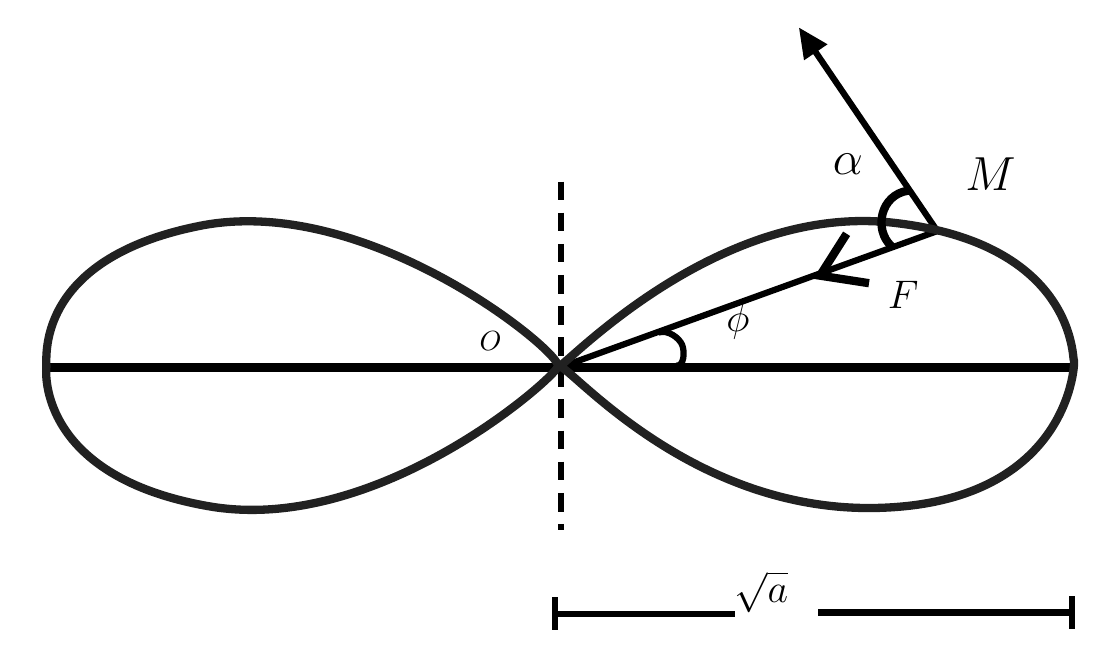
\begin{tikzpicture}[x=0.75pt,y=0.75pt,yscale=-1,xscale=1]
%uncomment if require: \path (0,718); %set diagram left start at 0, and has height of 718

%Straight Lines [id:da14907241164540275] 
\draw [line width=2.25]    (334.4,290.4) -- (421.4,290.4) ;
\draw [shift={(334.4,290.4)}, rotate = 180] [color={rgb, 255:red, 0; green, 0; blue, 0 }  ][line width=2.25]    (0,7.83) -- (0,-7.83)   ;
%Straight Lines [id:da8018641526158063] 
\draw [line width=2.25]    (461.4,289.8) -- (583.4,289.8) ;
\draw [shift={(583.4,289.8)}, rotate = 180] [color={rgb, 255:red, 0; green, 0; blue, 0 }  ][line width=2.25]    (0,7.83) -- (0,-7.83)   ;
%Straight Lines [id:da5328768952850804] 
\draw [line width=3]    (89.4,171.8) -- (296.4,171.8) -- (583.4,171.8) ;
%Straight Lines [id:da6002299620394058] 
\draw [line width=2.25]  [dash pattern={on 6.75pt off 4.5pt}]  (337.2,82.2) -- (337.2,101) -- (337.2,250.2) ;
%Straight Lines [id:da22746505400775097] 
\draw [line width=2.25]    (336.2,172) -- (451.07,130.49) -- (519.4,105.8) ;
\draw  [line width=3]  (485.76,131.19) -- (462.14,127.55) -- (474.96,107.37) ;
%Curve Lines [id:da6092247187578377] 
\draw [line width=2.25]    (384.4,154.93) .. controls (389.05,153.49) and (394.4,157.66) .. (395.73,160.93) .. controls (397.07,164.21) and (396.7,171.41) .. (392.87,170.93) ;
%Straight Lines [id:da2276044306388001] 
\draw [line width=2.25]    (517.67,104.6) -- (454.88,12.27) ;
\draw [shift={(452.07,8.13)}, rotate = 415.78] [fill={rgb, 255:red, 0; green, 0; blue, 0 }  ][line width=0.08]  [draw opacity=0] (14.29,-6.86) -- (0,0) -- (14.29,6.86) -- cycle    ;
%Shape: Polygon Curved [id:ds5559068249236452] 
\draw  [color={rgb, 255:red, 33; green, 33; blue, 33 }  ,draw opacity=1 ][line width=3]  (89.4,171.8) .. controls (89.8,168.9) and (82.4,119.65) .. (163.4,103.55) .. controls (244.4,87.45) and (338.3,164.9) .. (335.9,171.3) .. controls (333.5,177.7) and (408.65,92.05) .. (497.4,102.05) .. controls (586.15,112.05) and (583.65,168.8) .. (584.45,168.25) .. controls (585.25,167.7) and (583.65,237.05) .. (490.05,239.45) .. controls (396.45,241.85) and (337.5,165.7) .. (335.9,171.3) .. controls (334.3,176.9) and (248.9,252.8) .. (167.65,238.65) .. controls (86.4,224.5) and (89,174.7) .. (89.4,171.8) -- cycle ;
%Curve Lines [id:da9199004828768644] 
\draw [color={rgb, 255:red, 0; green, 0; blue, 0 }  ][line width=3] [line join = round][line cap = round]   (504.6,86.6) .. controls (491.27,88.5) and (487.8,105.4) .. (496.6,113.4) ;

% Text Node
\draw (419.6,268.6) node [anchor=north west][inner sep=0.75pt]  [font=\Large]  {$\sqrt{a}$};
% Text Node
\draw (493.6,129.2) node [anchor=north west][inner sep=0.75pt]  [font=\Large]  {$F$};
% Text Node
\draw (415.8,139.87) node [anchor=north west][inner sep=0.75pt]  [font=\Large]  {$\phi $};
% Text Node
\draw (467.13,67.73) node [anchor=north west][inner sep=0.75pt]  [font=\LARGE]  {$\alpha $};
% Text Node
\draw (530.87,69.73) node [anchor=north west][inner sep=0.75pt]  [font=\LARGE]  {$M$};
% Text Node
\draw (303.41,159.13) node    {$O$};
% Text Node


\end{tikzpicture}

\end{center}
If the expression for force is given as \[F = - \frac{K m V_{0}^{2} r_{0}^{2} a^2 \sin^2 \alpha}{r^7}\]
Find the value of $K$


\end{problem}
\begin{flushright}
\textbf{\Large{-Proposed by Harshit Gupta}}
\end{flushright}
\begin{solution}
{\Large{\textbf{Answer: 3}}}\\






%Type the solution here

The magnitude of central force:
$$F(r)=m({\ddot  {r}}-r{\dot  {\theta }}^{{2}})$$
Conservation of angular momentum gives us:
$$r^{{2}}{\dot  {\theta }}={\text{constant}}=L$$
$r$ can be converted into terms of $u=\frac{1}{r}$
$${\begin{aligned}&{\frac  {{\mathrm  {d}}u}{{\mathrm  {d}}\theta }}={\frac  {{\mathrm  {d}}}{{\mathrm  {d}}t}}\left({\frac  {1}{r}}\right){\frac  {{\mathrm  {d}}t}{{\mathrm  {d}}\theta }}=-{\frac  {{{\dot  {r}}}}{r^{{2}}{\dot  {\theta }}}}=-{\frac  {{{\dot  {r}}}}{L}}\\&{\frac  {{\mathrm  {d}}^{{2}}u}{{\mathrm  {d}}\theta ^{{2}}}}=-{\frac  {1}{L}}{\frac  {{\mathrm  {d}}{\dot  {r}}}{{\mathrm  {d}}t}}{\frac  {{\mathrm  {d}}t}{{\mathrm  {d}}\theta }}=-{\frac  {{{\ddot  {r}}}}{L{\dot  {\theta }}}}=-{\frac  {{{\ddot  {r}}}}{L^{{2}}u^{{2}}}}\\\end{aligned}}$$
Solving all the 3 equations we get the famous Binet Equation:

$\boxed{\displaystyle F(r) =-\frac{L^{2}}{mr^{2}}\left[ \ \frac{d^{2}}{d\phi ^{2}}\left(\frac{1}{r}\right) +\frac{1}{r}\right]}$ 

Now substituting $\displaystyle r=\sqrt{a\ \cos 2 \phi}$, $\displaystyle L=mv_{o} r_{o}\sin \alpha $ and differentiating wrt to $\phi$ we get:

$\displaystyle F=-\frac{3ma^2r_{o} v_{o}\sin^2 \alpha}{r^{3}\cos^{2}\phi}$ =$\displaystyle -\frac{3ma^2r_{o}^{2} v_{o}^{2}\sin^2 \alpha}{r^{7}}$ hence $\boxed{k=3}$









\end{solution}
\vspace{10mm}%\section{Problem 14}


\begin{problem}

We have a tesseract cubic style arrangement with voltmeters and resistances as shown in the figure. There are identical voltmeters to each side of smaller cube and side connecting to larger cube as shown in fig. below. All sides have equal resistance R, and across 2 ends of bigger cube connected with a battery of 300V. Calculate
$$\frac{7}{99}\sum_{i = 0}^{n} V_i,$$\\ where $V_i$ is reading of $i^{th}$ voltmeter

\begin{center}
    \includegraphics[width=\textwidth]{unknown.png}
\end{center}
\end{problem}
\begin{flushright}
\textbf{\Large{-Proposed by AKIII}}
\end{flushright}
\begin{solution}
{\Large{\textbf{Answer: 40}}}\\


\begin{center}
    

\tikzset{every picture/.style={line width=0.75pt}} %set default line width to 0.75pt        

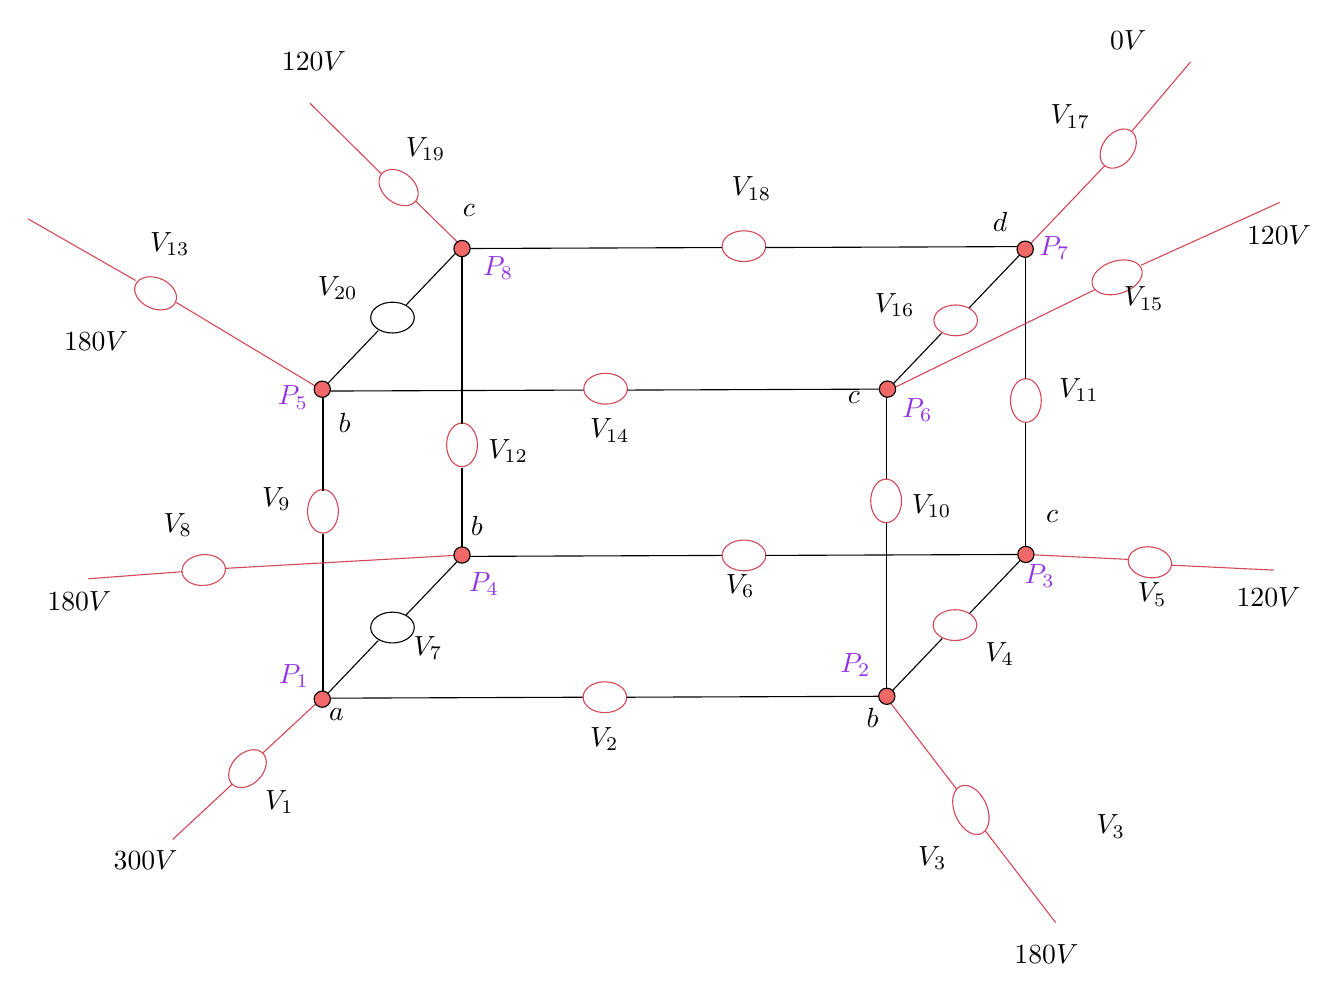
\begin{tikzpicture}[x=0.75pt,y=0.75pt,yscale=-1,xscale=1]
%uncomment if require: \path (0,486); %set diagram left start at 0, and has height of 486

%Straight Lines [id:da6650256016491007] 
\draw    (183.67,304.08) -- (156.67,332.35) ;
%Straight Lines [id:da24003330587970817] 
\draw    (224,263.56) -- (197,291.83) ;
%Shape: Ellipse [id:dp6811067019919566] 
\draw   (180,297.84) .. controls (180,293.74) and (184.7,290.42) .. (190.5,290.42) .. controls (196.3,290.42) and (201,293.74) .. (201,297.84) .. controls (201,301.94) and (196.3,305.26) .. (190.5,305.26) .. controls (184.7,305.26) and (180,301.94) .. (180,297.84) -- cycle ;
%Straight Lines [id:da5456050055817654] 
\draw    (224,263.56) -- (349.33,263.09) ;
%Shape: Ellipse [id:dp12459714298304458] 
\draw  [color={rgb, 255:red, 211; green, 73; blue, 89 }  ,draw opacity=1 ] (349.33,263.09) .. controls (349.33,258.99) and (354.03,255.67) .. (359.83,255.67) .. controls (365.63,255.67) and (370.33,258.99) .. (370.33,263.09) .. controls (370.33,267.19) and (365.63,270.51) .. (359.83,270.51) .. controls (354.03,270.51) and (349.33,267.19) .. (349.33,263.09) -- cycle ;
%Straight Lines [id:da27034180226072024] 
\draw    (370.33,263.09) -- (495.67,262.62) ;
%Straight Lines [id:da6463711208251399] 
\draw    (455.33,303.14) -- (428.33,331.41) ;
%Straight Lines [id:da3773500159043368] 
\draw    (495.67,262.62) -- (468.67,290.89) ;
%Shape: Ellipse [id:dp5921069767621325] 
\draw  [color={rgb, 255:red, 211; green, 73; blue, 89 }  ,draw opacity=1 ] (451,296.66) .. controls (451,292.56) and (455.7,289.24) .. (461.5,289.24) .. controls (467.3,289.24) and (472,292.56) .. (472,296.66) .. controls (472,300.76) and (467.3,304.08) .. (461.5,304.08) .. controls (455.7,304.08) and (451,300.76) .. (451,296.66) -- cycle ;
%Straight Lines [id:da38672178795424084] 
\draw    (157,331.88) -- (282.33,331.41) ;
%Shape: Ellipse [id:dp4287034042442355] 
\draw  [color={rgb, 255:red, 211; green, 73; blue, 89 }  ,draw opacity=1 ] (282.33,331.41) .. controls (282.33,327.31) and (287.03,323.99) .. (292.83,323.99) .. controls (298.63,323.99) and (303.33,327.31) .. (303.33,331.41) .. controls (303.33,335.51) and (298.63,338.83) .. (292.83,338.83) .. controls (287.03,338.83) and (282.33,335.51) .. (282.33,331.41) -- cycle ;
%Straight Lines [id:da44788116034739867] 
\draw    (303.33,331.41) -- (428.67,330.94) ;
%Straight Lines [id:da001164528135337406] 
\draw    (224,221) -- (224,263.56) ;
%Straight Lines [id:da8036441425111314] 
\draw    (157,253) -- (157,331.88) ;
%Straight Lines [id:da30428190136863487] 
\draw    (428.33,247.33) -- (428.33,331.41) ;
%Straight Lines [id:da839572889411367] 
\draw    (495.67,198.95) -- (495.67,262.62) ;
%Shape: Ellipse [id:dp6544178371085012] 
\draw  [color={rgb, 255:red, 211; green, 73; blue, 89 }  ,draw opacity=1 ] (495.67,177.95) .. controls (499.77,177.95) and (503.09,182.65) .. (503.09,188.45) .. controls (503.09,194.25) and (499.77,198.95) .. (495.67,198.95) .. controls (491.57,198.95) and (488.25,194.25) .. (488.25,188.45) .. controls (488.25,182.65) and (491.57,177.95) .. (495.67,177.95) -- cycle ;
%Shape: Ellipse [id:dp24605488483901028] 
\draw  [color={rgb, 255:red, 211; green, 73; blue, 89 }  ,draw opacity=1 ] (428.33,226.33) .. controls (432.43,226.33) and (435.75,231.03) .. (435.75,236.83) .. controls (435.75,242.63) and (432.43,247.33) .. (428.33,247.33) .. controls (424.23,247.33) and (420.91,242.63) .. (420.91,236.83) .. controls (420.91,231.03) and (424.23,226.33) .. (428.33,226.33) -- cycle ;
%Shape: Ellipse [id:dp36464003227716346] 
\draw  [color={rgb, 255:red, 211; green, 73; blue, 89 }  ,draw opacity=1 ] (157,231.33) .. controls (161.1,231.33) and (164.42,236.03) .. (164.42,241.83) .. controls (164.42,247.63) and (161.1,252.33) .. (157,252.33) .. controls (152.9,252.33) and (149.58,247.63) .. (149.58,241.83) .. controls (149.58,236.03) and (152.9,231.33) .. (157,231.33) -- cycle ;
%Shape: Ellipse [id:dp2614241974361393] 
\draw  [color={rgb, 255:red, 211; green, 73; blue, 89 }  ,draw opacity=1 ] (224,199.33) .. controls (228.1,199.33) and (231.42,204.03) .. (231.42,209.83) .. controls (231.42,215.63) and (228.1,220.33) .. (224,220.33) .. controls (219.9,220.33) and (216.58,215.63) .. (216.58,209.83) .. controls (216.58,204.03) and (219.9,199.33) .. (224,199.33) -- cycle ;
%Straight Lines [id:da4765245431225309] 
\draw    (224,115.23) -- (224,200) ;
%Straight Lines [id:da2681294140834023] 
\draw    (495.67,114.29) -- (495.67,177.95) ;
%Straight Lines [id:da20697589200959499] 
\draw    (428.33,183.08) -- (428.33,226.33) ;
%Straight Lines [id:da43008748521096796] 
\draw    (157,183.55) -- (157,232) ;
%Straight Lines [id:da5954636506177831] 
\draw    (183.67,154.75) -- (156.67,183.02) ;
%Straight Lines [id:da26200526156051196] 
\draw    (224,114.23) -- (197,142.5) ;
%Shape: Ellipse [id:dp7337576601229325] 
\draw   (180,148.51) .. controls (180,144.41) and (184.7,141.08) .. (190.5,141.08) .. controls (196.3,141.08) and (201,144.41) .. (201,148.51) .. controls (201,152.6) and (196.3,155.93) .. (190.5,155.93) .. controls (184.7,155.93) and (180,152.6) .. (180,148.51) -- cycle ;
%Straight Lines [id:da8709911741706231] 
\draw    (455,156.08) -- (428,184.35) ;
%Straight Lines [id:da8032089584760294] 
\draw    (495.33,115.56) -- (468.33,143.83) ;
%Shape: Ellipse [id:dp5628384963792685] 
\draw  [color={rgb, 255:red, 211; green, 73; blue, 89 }  ,draw opacity=1 ] (451.33,149.84) .. controls (451.33,145.74) and (456.03,142.42) .. (461.83,142.42) .. controls (467.63,142.42) and (472.33,145.74) .. (472.33,149.84) .. controls (472.33,153.94) and (467.63,157.26) .. (461.83,157.26) .. controls (456.03,157.26) and (451.33,153.94) .. (451.33,149.84) -- cycle ;
%Straight Lines [id:da2626860426519493] 
\draw    (224,115.23) -- (349.33,114.76) ;
%Shape: Ellipse [id:dp5933561689975362] 
\draw  [color={rgb, 255:red, 211; green, 73; blue, 89 }  ,draw opacity=1 ] (349.33,114.09) .. controls (349.33,109.99) and (354.03,106.67) .. (359.83,106.67) .. controls (365.63,106.67) and (370.33,109.99) .. (370.33,114.09) .. controls (370.33,118.19) and (365.63,121.51) .. (359.83,121.51) .. controls (354.03,121.51) and (349.33,118.19) .. (349.33,114.09) -- cycle ;
%Straight Lines [id:da9097826761403298] 
\draw    (370.33,114.76) -- (495.67,114.29) ;
%Straight Lines [id:da5311029337875597] 
\draw    (157.33,183.9) -- (282.67,183.43) ;
%Shape: Ellipse [id:dp1614656605412803] 
\draw  [color={rgb, 255:red, 211; green, 73; blue, 89 }  ,draw opacity=1 ] (282.67,182.76) .. controls (282.67,178.66) and (287.37,175.34) .. (293.17,175.34) .. controls (298.97,175.34) and (303.67,178.66) .. (303.67,182.76) .. controls (303.67,186.86) and (298.97,190.18) .. (293.17,190.18) .. controls (287.37,190.18) and (282.67,186.86) .. (282.67,182.76) -- cycle ;
%Straight Lines [id:da470404963386827] 
\draw    (303.67,183.43) -- (429,182.95) ;
%Straight Lines [id:da12307015544782818] 
\draw [color={rgb, 255:red, 211; green, 73; blue, 89 }  ,draw opacity=1 ]   (428.33,331.41) -- (462.28,375.7) ;
%Straight Lines [id:da18957502626198974] 
\draw [color={rgb, 255:red, 211; green, 73; blue, 89 }  ,draw opacity=1 ]   (495.67,262.62) -- (545,265) ;
%Straight Lines [id:da659036272011406] 
\draw [color={rgb, 255:red, 211; green, 73; blue, 89 }  ,draw opacity=1 ]   (495.33,115.56) -- (533.67,75.33) ;
%Straight Lines [id:da3572963019066744] 
\draw [color={rgb, 255:red, 211; green, 73; blue, 89 }  ,draw opacity=1 ]   (224,114.33) -- (201.67,92.39) ;
%Straight Lines [id:da13991802440153678] 
\draw [color={rgb, 255:red, 211; green, 73; blue, 89 }  ,draw opacity=1 ]   (128,358.33) -- (156.67,331.69) ;
%Straight Lines [id:da8718691787890278] 
\draw [color={rgb, 255:red, 211; green, 73; blue, 89 }  ,draw opacity=1 ]   (110,269.33) -- (224,262.89) ;
%Straight Lines [id:da2900600177210051] 
\draw [color={rgb, 255:red, 211; green, 73; blue, 89 }  ,draw opacity=1 ]   (44,274.33) -- (89.06,270.95) ;
%Shape: Ellipse [id:dp6754643203012942] 
\draw  [color={rgb, 255:red, 211; green, 73; blue, 89 }  ,draw opacity=1 ] (113.27,373.3) .. controls (110.35,370.43) and (111.28,364.75) .. (115.35,360.61) .. controls (119.41,356.48) and (125.08,355.46) .. (128,358.33) .. controls (130.92,361.21) and (129.99,366.89) .. (125.92,371.02) .. controls (121.86,375.16) and (116.19,376.18) .. (113.27,373.3) -- cycle ;
%Straight Lines [id:da647159242001045] 
\draw [color={rgb, 255:red, 211; green, 73; blue, 89 }  ,draw opacity=1 ]   (84.6,399.95) -- (113.27,373.3) ;
%Shape: Ellipse [id:dp9686971845423358] 
\draw  [color={rgb, 255:red, 211; green, 73; blue, 89 }  ,draw opacity=1 ] (476.05,395.71) .. controls (473.06,399.22) and (467.55,397.58) .. (463.75,392.05) .. controls (459.94,386.53) and (459.29,379.21) .. (462.28,375.7) .. controls (465.28,372.2) and (470.79,373.83) .. (474.59,379.36) .. controls (478.39,384.88) and (479.05,392.2) .. (476.05,395.71) -- cycle ;
%Straight Lines [id:da8173262056767658] 
\draw [color={rgb, 255:red, 211; green, 73; blue, 89 }  ,draw opacity=1 ]   (476.05,395.71) -- (510,440) ;
%Shape: Ellipse [id:dp8480539540571013] 
\draw  [color={rgb, 255:red, 211; green, 73; blue, 89 }  ,draw opacity=1 ] (565.81,267.78) .. controls (565.27,271.85) and (560.17,274.52) .. (554.42,273.75) .. controls (548.68,272.98) and (544.46,269.06) .. (545,265) .. controls (545.54,260.94) and (550.64,258.27) .. (556.39,259.04) .. controls (562.14,259.81) and (566.36,263.72) .. (565.81,267.78) -- cycle ;
%Straight Lines [id:da25314030622878847] 
\draw [color={rgb, 255:red, 211; green, 73; blue, 89 }  ,draw opacity=1 ]   (565.81,267.78) -- (615.15,270.17) ;
%Shape: Ellipse [id:dp46667010607049475] 
\draw  [color={rgb, 255:red, 211; green, 73; blue, 89 }  ,draw opacity=1 ] (546.62,58.81) .. controls (549.85,61.33) and (549.56,67.08) .. (545.99,71.65) .. controls (542.41,76.21) and (536.89,77.86) .. (533.67,75.33) .. controls (530.44,72.8) and (530.73,67.06) .. (534.3,62.49) .. controls (537.88,57.93) and (543.4,56.28) .. (546.62,58.81) -- cycle ;
%Straight Lines [id:da7804302600825126] 
\draw [color={rgb, 255:red, 211; green, 73; blue, 89 }  ,draw opacity=1 ]   (546.62,58.81) -- (575,25.33) ;
%Straight Lines [id:da8806458810644593] 
\draw [color={rgb, 255:red, 211; green, 73; blue, 89 }  ,draw opacity=1 ]   (185.22,79.34) -- (150.75,45.24) ;
%Shape: Ellipse [id:dp45205095850646204] 
\draw  [color={rgb, 255:red, 211; green, 73; blue, 89 }  ,draw opacity=1 ] (201.67,92.39) .. controls (199.12,95.6) and (193.37,95.28) .. (188.83,91.68) .. controls (184.29,88.07) and (182.67,82.55) .. (185.22,79.34) .. controls (187.76,76.13) and (193.51,76.45) .. (198.05,80.05) .. controls (202.6,83.65) and (204.21,89.18) .. (201.67,92.39) -- cycle ;
%Shape: Ellipse [id:dp4977854349690931] 
\draw  [color={rgb, 255:red, 211; green, 73; blue, 89 }  ,draw opacity=1 ] (89.06,270.95) .. controls (88.75,266.87) and (93.18,263.19) .. (98.96,262.74) .. controls (104.74,262.3) and (109.68,265.25) .. (110,269.33) .. controls (110.32,273.42) and (105.88,277.09) .. (100.1,277.54) .. controls (94.32,277.99) and (89.38,275.04) .. (89.06,270.95) -- cycle ;
%Straight Lines [id:da7385540461476401] 
\draw [color={rgb, 255:red, 211; green, 73; blue, 89 }  ,draw opacity=1 ]   (86,141) -- (157.33,183.9) ;
%Straight Lines [id:da4649749450989644] 
\draw [color={rgb, 255:red, 211; green, 73; blue, 89 }  ,draw opacity=1 ]   (15,101) -- (66.74,130.63) ;
%Shape: Ellipse [id:dp24469705711896972] 
\draw  [color={rgb, 255:red, 211; green, 73; blue, 89 }  ,draw opacity=1 ] (66.74,132.63) .. controls (68.38,128.87) and (74.01,127.69) .. (79.33,130.01) .. controls (84.65,132.32) and (87.63,137.24) .. (86,141) .. controls (84.37,144.76) and (78.73,145.93) .. (73.41,143.62) .. controls (68.09,141.31) and (65.11,136.39) .. (66.74,132.63) -- cycle ;
%Straight Lines [id:da9894389717408159] 
\draw [color={rgb, 255:red, 211; green, 73; blue, 89 }  ,draw opacity=1 ]   (428,184.35) -- (529,135) ;
%Straight Lines [id:da9010366481235499] 
\draw [color={rgb, 255:red, 211; green, 73; blue, 89 }  ,draw opacity=1 ]   (551.25,123.24) -- (618,93) ;
%Shape: Ellipse [id:dp6518702944381425] 
\draw  [color={rgb, 255:red, 211; green, 73; blue, 89 }  ,draw opacity=1 ] (550.25,123.24) .. controls (553.45,126.56) and (551.29,131.89) .. (545.42,135.13) .. controls (539.55,138.38) and (532.2,138.32) .. (529,135) .. controls (525.8,131.68) and (527.97,126.35) .. (533.84,123.11) .. controls (539.71,119.86) and (547.06,119.92) .. (550.25,123.24) -- cycle ;
%Shape: Circle [id:dp3777705919104657] 
\draw  [fill={rgb, 255:red, 240; green, 104; blue, 104 }  ,fill opacity=1 ] (152.74,332.35) .. controls (152.74,330.19) and (154.5,328.43) .. (156.67,328.43) .. controls (158.83,328.43) and (160.59,330.19) .. (160.59,332.35) .. controls (160.59,334.52) and (158.83,336.28) .. (156.67,336.28) .. controls (154.5,336.28) and (152.74,334.52) .. (152.74,332.35) -- cycle ;
%Shape: Circle [id:dp21923921461984341] 
\draw  [fill={rgb, 255:red, 240; green, 104; blue, 104 }  ,fill opacity=1 ] (424.74,330.94) .. controls (424.74,328.77) and (426.5,327.02) .. (428.67,327.02) .. controls (430.83,327.02) and (432.59,328.77) .. (432.59,330.94) .. controls (432.59,333.11) and (430.83,334.86) .. (428.67,334.86) .. controls (426.5,334.86) and (424.74,333.11) .. (424.74,330.94) -- cycle ;
%Shape: Circle [id:dp3873186337053345] 
\draw  [fill={rgb, 255:red, 240; green, 104; blue, 104 }  ,fill opacity=1 ] (491.74,262.62) .. controls (491.74,260.45) and (493.5,258.69) .. (495.67,258.69) .. controls (497.83,258.69) and (499.59,260.45) .. (499.59,262.62) .. controls (499.59,264.78) and (497.83,266.54) .. (495.67,266.54) .. controls (493.5,266.54) and (491.74,264.78) .. (491.74,262.62) -- cycle ;
%Shape: Circle [id:dp03017054547146869] 
\draw  [fill={rgb, 255:red, 240; green, 104; blue, 104 }  ,fill opacity=1 ] (220.08,262.89) .. controls (220.08,260.73) and (221.83,258.97) .. (224,258.97) .. controls (226.17,258.97) and (227.92,260.73) .. (227.92,262.89) .. controls (227.92,265.06) and (226.17,266.81) .. (224,266.81) .. controls (221.83,266.81) and (220.08,265.06) .. (220.08,262.89) -- cycle ;
%Shape: Circle [id:dp6685070910931468] 
\draw  [fill={rgb, 255:red, 240; green, 104; blue, 104 }  ,fill opacity=1 ] (491.41,115.56) .. controls (491.41,113.39) and (493.17,111.64) .. (495.33,111.64) .. controls (497.5,111.64) and (499.26,113.39) .. (499.26,115.56) .. controls (499.26,117.73) and (497.5,119.48) .. (495.33,119.48) .. controls (493.17,119.48) and (491.41,117.73) .. (491.41,115.56) -- cycle ;
%Shape: Circle [id:dp4181078302501793] 
\draw  [fill={rgb, 255:red, 240; green, 104; blue, 104 }  ,fill opacity=1 ] (425.08,182.95) .. controls (425.08,180.79) and (426.83,179.03) .. (429,179.03) .. controls (431.17,179.03) and (432.92,180.79) .. (432.92,182.95) .. controls (432.92,185.12) and (431.17,186.88) .. (429,186.88) .. controls (426.83,186.88) and (425.08,185.12) .. (425.08,182.95) -- cycle ;
%Shape: Circle [id:dp841872736630298] 
\draw  [fill={rgb, 255:red, 240; green, 104; blue, 104 }  ,fill opacity=1 ] (220.08,115.23) .. controls (220.08,113.06) and (221.83,111.31) .. (224,111.31) .. controls (226.17,111.31) and (227.92,113.06) .. (227.92,115.23) .. controls (227.92,117.4) and (226.17,119.15) .. (224,119.15) .. controls (221.83,119.15) and (220.08,117.4) .. (220.08,115.23) -- cycle ;
%Shape: Circle [id:dp9299149395422728] 
\draw  [fill={rgb, 255:red, 240; green, 104; blue, 104 }  ,fill opacity=1 ] (152.74,183.02) .. controls (152.74,180.85) and (154.5,179.1) .. (156.67,179.1) .. controls (158.83,179.1) and (160.59,180.85) .. (160.59,183.02) .. controls (160.59,185.19) and (158.83,186.94) .. (156.67,186.94) .. controls (154.5,186.94) and (152.74,185.19) .. (152.74,183.02) -- cycle ;

% Text Node
\draw (158.67,335.75) node [anchor=north west][inner sep=0.75pt]    {$a$};
% Text Node
\draw (504.17,240.25) node [anchor=north west][inner sep=0.75pt]    {$c$};
% Text Node
\draw (417.67,335.25) node [anchor=north west][inner sep=0.75pt]    {$b$};
% Text Node
\draw (227,243.18) node [anchor=north west][inner sep=0.75pt]    {$b$};
% Text Node
\draw (478.5,96.68) node [anchor=north west][inner sep=0.75pt]    {$d$};
% Text Node
\draw (408.67,182.75) node [anchor=north west][inner sep=0.75pt]    {$c$};
% Text Node
\draw (163.33,193.3) node [anchor=north west][inner sep=0.75pt]    {$b$};
% Text Node
\draw (223.17,92.75) node [anchor=north west][inner sep=0.75pt]    {$c$};
% Text Node
\draw (127.92,375.09) node [anchor=north west][inner sep=0.75pt]    {$V_{1}$};
% Text Node
\draw (284.42,344.59) node [anchor=north west][inner sep=0.75pt]    {$V_{2}$};
% Text Node
\draw (442.45,401.92) node [anchor=north west][inner sep=0.75pt]    {$V_{3}$};
% Text Node
\draw (474.92,303.59) node [anchor=north west][inner sep=0.75pt]    {$V_{4}$};
% Text Node
\draw (548.42,275.09) node [anchor=north west][inner sep=0.75pt]    {$V_{5}$};
% Text Node
\draw (349.92,271.09) node [anchor=north west][inner sep=0.75pt]    {$V_{6}$};
% Text Node
\draw (199.42,301.09) node [anchor=north west][inner sep=0.75pt]    {$V_{7}$};
% Text Node
\draw (78.92,241.59) node [anchor=north west][inner sep=0.75pt]    {$V_{8}$};
% Text Node
\draw (126.42,229.09) node [anchor=north west][inner sep=0.75pt]    {$V_{9}$};
% Text Node
\draw (439.42,232.59) node [anchor=north west][inner sep=0.75pt]    {$V_{10}$};
% Text Node
\draw (510.42,176.59) node [anchor=north west][inner sep=0.75pt]    {$V_{11}$};
% Text Node
\draw (235.42,206.09) node [anchor=north west][inner sep=0.75pt]    {$V_{12}$};
% Text Node
\draw (72.42,106.09) node [anchor=north west][inner sep=0.75pt]    {$V_{13}$};
% Text Node
\draw (284.42,196.09) node [anchor=north west][inner sep=0.75pt]    {$V_{14}$};
% Text Node
\draw (541.63,132.52) node [anchor=north west][inner sep=0.75pt]    {$V_{15}$};
% Text Node
\draw (528.45,386.92) node [anchor=north west][inner sep=0.75pt]    {$V_{3}$};
% Text Node
\draw (421.63,135.52) node [anchor=north west][inner sep=0.75pt]    {$V_{16}$};
% Text Node
\draw (506.29,44.85) node [anchor=north west][inner sep=0.75pt]    {$V_{17}$};
% Text Node
\draw (352.63,79.52) node [anchor=north west][inner sep=0.75pt]    {$V_{18}$};
% Text Node
\draw (195.63,60.52) node [anchor=north west][inner sep=0.75pt]    {$V_{19}$};
% Text Node
\draw (153.29,127.52) node [anchor=north west][inner sep=0.75pt]    {$V_{20}$};
% Text Node
\draw (54.92,404.09) node [anchor=north west][inner sep=0.75pt]    {$300V$};
% Text Node
\draw (488.92,449.09) node [anchor=north west][inner sep=0.75pt]    {$180V$};
% Text Node
\draw (595.92,277.09) node [anchor=north west][inner sep=0.75pt]    {$120V$};
% Text Node
\draw (601,103.09) node [anchor=north west][inner sep=0.75pt]    {$120V$};
% Text Node
\draw (535,9.09) node [anchor=north west][inner sep=0.75pt]    {$0V$};
% Text Node
\draw (136,19.09) node [anchor=north west][inner sep=0.75pt]    {$120V$};
% Text Node
\draw (31,154.09) node [anchor=north west][inner sep=0.75pt]    {$180V$};
% Text Node
\draw (23,279.09) node [anchor=north west][inner sep=0.75pt]    {$180V$};
% Text Node
\draw (134.5,314.4) node [anchor=north west][inner sep=0.75pt]  [color={rgb, 255:red, 146; green, 51; blue, 230 }  ,opacity=1 ]  {$P_{1}$};
% Text Node
\draw (405,308.9) node [anchor=north west][inner sep=0.75pt]  [color={rgb, 255:red, 146; green, 51; blue, 230 }  ,opacity=1 ]  {$P_{2}$};
% Text Node
\draw (493.74,266.02) node [anchor=north west][inner sep=0.75pt]  [color={rgb, 255:red, 146; green, 51; blue, 230 }  ,opacity=1 ]  {$P_{3}$};
% Text Node
\draw (226,270.21) node [anchor=north west][inner sep=0.75pt]  [color={rgb, 255:red, 146; green, 51; blue, 230 }  ,opacity=1 ]  {$P_{4}$};
% Text Node
\draw (134,180.21) node [anchor=north west][inner sep=0.75pt]  [color={rgb, 255:red, 146; green, 51; blue, 230 }  ,opacity=1 ]  {$P_{5}$};
% Text Node
\draw (434.92,186.35) node [anchor=north west][inner sep=0.75pt]  [color={rgb, 255:red, 146; green, 51; blue, 230 }  ,opacity=1 ]  {$P_{6}$};
% Text Node
\draw (500.92,108.35) node [anchor=north west][inner sep=0.75pt]  [color={rgb, 255:red, 146; green, 51; blue, 230 }  ,opacity=1 ]  {$P_{7}$};
% Text Node
\draw (232.92,117.85) node [anchor=north west][inner sep=0.75pt]  [color={rgb, 255:red, 146; green, 51; blue, 230 }  ,opacity=1 ]  {$P_{8}$};


\end{tikzpicture}

\end{center}

Applying KCL at P1:

\hspace{7.5cm}$\frac{a-300}{R}+3\left( \frac{a-b}{R}\right)=0$ 
\begin{equation*}
    \Rightarrow 4a=300+3b
\end{equation*}\\

Applying KCL at P7: 

\hspace{7.5cm}$\frac{d}{R}+3\left(\frac{d-c}{R}\right)=0$
\begin{equation*}
   \hspace{-1cm} \Rightarrow 4d=3c
\end{equation*}

Applying KCL at P2:

\hspace{7.5cm} $\frac{b-180}{R}+2\left(\frac{b-c}{R}\right)+\frac{b-a}{R}=0$
\begin{equation*}
    \hspace{0.8cm}\Rightarrow 4b=a+2c+180
\end{equation*}

Applying KCL at P3:

\hspace{7.5cm}$\frac{c-d}{R}+2\left(\frac{c-b}{R}\right)+\frac{c-120}{R}=0$
\begin{equation*}
    \hspace{0.95cm}\Rightarrow 4c=d+2b+120
\end{equation*}

\hspace{6cm}$\rightarrow\frac{13}{4}c=2b+120$ \hspace{1cm}...from (2)\\

So, 
$$26b=16c+2090$$
$$26c=16b+960$$

\begin{tikzpicture}
\hspace{7.2cm}\draw (8,0) -- (11.5,0);
\end{tikzpicture}

By solving, 

\hspace{7cm}$a=\frac{1380}{7}V$, $b=\frac{1140}{7}V$, $c=\frac{960}{7}V$, $d=\frac{720}{7}V$\\
\vspace{1cm}

$\rightarrow V_1=300-a$, $V_2=V_7=V_9=a-b$, $V_3=V_8=V_{13}=b-180$\\

$\rightarrow V_4=V_{10}=V_6=V_{12}=V_{14}=V_2=b-c$\\

$\rightarrow V_5=V_{15}=V_{19}=c-120$\\

$\rightarrow V_{11}=V_{16}=V_{18}=c-d$, $V_{17}=d$\\
\pagebreak 
$$\Rightarrow \frac{7}{99}\sum_{i=1}^{20} V_i=\frac{7}{99}(300-a+3a-3b+3b-540+6b-6c+3c-360+3c-3d+d)$$

$$=\frac{7}{99}\left(\frac{3960}{7}\right)=40$$
\end{solution}
\vspace{10mm}%\section{Problem 15}

\begin{problem}





\textbf{Power radiated by a point charge:}
$$P= k \mu_{0}^{d} q^e \zeta^f c^g$$ where k is a dimensionless constant. Here, $\mu_0$ is the permeability of free space, $q$ is the charge, $\zeta$ is the acceleration, and $c$ is the speed of light in vacuum.


Consider a fixed positive charge Q situated at fixed point in space (vacuum). At some instant, a $Li^{+3}$ ion (stable enough throughout the problem) is fired from infinity directly towards the charge $Q$ with a velocity $v_0$. The ion makes a shortest distance of approach to the fixed charge $x_0$ $(x_0 > 0)$.
Atharva (using his supernatural powers) extracts energy radiated away by $Li^{+3}$ ion during its whole journey and with that energy, excites an $H$ atom from ground state to third excited state. 
Ignore relativistic effects (i.e. $v_0 << c$), and radiative losses on the motion of the particle. Neglect all kind of particle physics interactions. 

If $\frac{mv_{0}^5}{Q} = \psi^4 \times 10^{25}$, where $m$ is the mass of ion, report $[\psi]$ where $[.]$ is the greatest integer function.
Take k = $\frac{1}{6 \pi}$ in the expression of power radiated by a point charge. \\
 You may find this integral helpful : 
$$\int_{\xi}^{\infty} \frac{1}{x^4 \sqrt{\frac{1}{\xi} - \frac{1}{x}}} dx = \frac{16}{15 \xi^{5/2}}$$
\end{problem}
\begin{flushright}
\textbf{\Large{-Proposed by Tarpan Ghosh}}
\end{flushright}
\begin{solution}
{\Large{\textbf{Answer: 2}}}\\
First, we calculate the exact expression for power radiated by a point when accelerated. Using dimensional analysis, it can be shown: \[P=k \frac{\mu_0 q^2 \zeta^2}{c}
\] This implies, the rate of work done is \[\frac{dW}{dt} = k \frac{\mu_0 q^2 \zeta^2}{c}\]


Let the charge of $Li^{+3} $ be $q$ and using Coulomb's law, \[\zeta =\frac{Qq}{4 \pi \epsilon_0 m x^2 } = \frac{\Omega}{x^2}\] where $\Omega = \frac{Qq}{4 \pi \epsilon_0 m}$

Therefore, the total energy radiated is (since total energy emitted is double of the energy emitted in a single cycle)  \[W = 2 \cdot \frac{k \Omega^2 \mu_0 q^2}{c} \int_{x_0}^{\infty} \frac{1}{v \cdot x^4} dx\]

Now applying conservation of energy (no radiative losses as given in question) \[v^2 = v_{0}^{2} - \frac{2 \Omega}{x}\]
$x_0 = \frac{2 \Omega}{v_{0}^2}$
Therefore,  \[W = 2 \cdot \frac{k \Omega^2 \mu_0 q^2}{c} \int_{x_0}^{\infty} \frac{1}{v \cdot x^4} dx = 2 \cdot \frac{k \Omega^2 \mu_0 q^2}{c} \int_{x_0}^{\infty} \frac{1}{x^4 \sqrt{v_{0} - \frac{2 \Omega}{x}}}dx = \frac{2 k \Omega^2 \mu_0 q^2}{c \sqrt{2 \Omega}} \int_{x_0}^{\infty} \frac{1}{x^4 \sqrt{\frac{1}{x_0} - \frac{1}{x}}} dx\]
Using the integral given in the problem, and further simplifications, we get total energy dissipated  \[E = \frac{8qm}{45 c^3 Q} v_{0}^5\]

Since Atharva is using this energy to excite the ground state single electron in $H$ atom, we can write 
\[\frac{8em}{15 c^3 Q} v_{0}^5 = 13.6 Z e \left( \frac{1}{n_{1}^2} - \frac{1}{n_{2}^2} \right)\]

Substituting all the values, we $\frac{m v_{0}^5}{Q} = 64.5468 \times 10^{25}$.
By comparing, we get $\psi = 2.834449208$. \\
Hence, $[\psi] = 2$ 
\qedsymbol

\end{solution}
\vspace{10mm}%\section{Problem 16}
\begin{problem}


A uniformly charged ring of radius $\boldsymbol{R}_{o}$ and total charge on the ring is $\boldsymbol{Q}_{o}$. There is a point $\boldsymbol{P}$ by a very small distance of $\boldsymbol{x}\left(\boldsymbol{x}<<\boldsymbol{R}_{o}\right)$ from the centre C in the plane of the ring as shown , The magnitude of electric field at point $\boldsymbol{P}$ due to the stationary ring is $\boldsymbol{E}_{o}$. Now the ring is rotated with constant angular velocity of $\boldsymbol{w}_{o}$ about an axis passing through its centre and perpendicular to the plane of the ring, The magnitude of magnetic field at point $\boldsymbol{P}$ due to the rotating ring is $\boldsymbol{B}_{o}$. Then the ratio of $\boldsymbol{E}_{o} / \boldsymbol{B}_{o}$ at point $\boldsymbol{P}$ is of the form $$ \frac{E_{o}}{B_{o}}=\frac{\alpha x c^{2}}{\omega\left[\beta R^{2}+\gamma  x^{2}\right]}$$ Where $\alpha, \beta$ and $\gamma $ are Integers and $c$ is speed of light. Compute $(\alpha+\beta+\gamma)$.
\vspace{5mm}
\begin{center}
    

\tikzset{every picture/.style={line width=0.75pt}} %set default line width to 0.75pt        

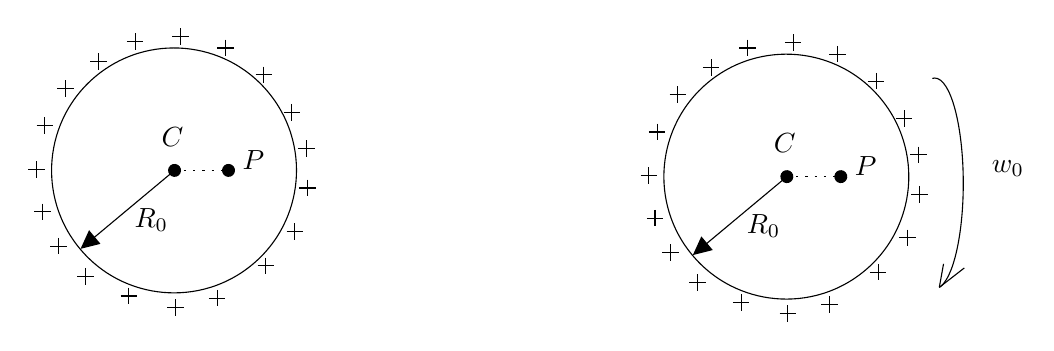
\begin{tikzpicture}[x=0.75pt,y=0.75pt,yscale=-1,xscale=1]
%uncomment if require: \path (0,300); %set diagram left start at 0, and has height of 300

%Shape: Circle [id:dp7761164188167768] 
\draw   (132.95,104.7) .. controls (157.97,83.82) and (195.18,87.18) .. (216.05,112.2) .. controls (236.93,137.22) and (233.57,174.43) .. (208.55,195.3) .. controls (183.53,216.18) and (146.32,212.82) .. (125.45,187.8) .. controls (104.57,162.78) and (107.93,125.57) .. (132.95,104.7) -- cycle ;
%Shape: Circle [id:dp8935842681351884] 
\draw  [fill={rgb, 255:red, 0; green, 0; blue, 0 }  ,fill opacity=1 ] (169.18,147.81) .. controls (170.38,146.81) and (172.18,146.97) .. (173.19,148.18) .. controls (174.19,149.38) and (174.03,151.18) .. (172.82,152.19) .. controls (171.62,153.19) and (169.82,153.03) .. (168.81,151.82) .. controls (167.81,150.62) and (167.97,148.82) .. (169.18,147.81) -- cycle ;
%Straight Lines [id:da9689860168746676] 
\draw    (171,150) -- (128,185.88) ;
\draw [shift={(125.7,187.8)}, rotate = 320.15999999999997] [fill={rgb, 255:red, 0; green, 0; blue, 0 }  ][line width=0.08]  [draw opacity=0] (8.93,-4.29) -- (0,0) -- (8.93,4.29) -- cycle    ;
%Shape: Circle [id:dp8150810955115602] 
\draw  [fill={rgb, 255:red, 0; green, 0; blue, 0 }  ,fill opacity=1 ] (195.18,147.81) .. controls (196.38,146.81) and (198.18,146.97) .. (199.19,148.18) .. controls (200.19,149.38) and (200.03,151.18) .. (198.82,152.19) .. controls (197.62,153.19) and (195.82,153.03) .. (194.81,151.82) .. controls (193.81,150.62) and (193.97,148.82) .. (195.18,147.81) -- cycle ;
\draw   (170,85.5) -- (178,85.5)(174,81.5) -- (174,89.5) ;
\draw   (191.5,91) -- (199.5,91)(195.5,87) -- (195.5,95) ;
\draw   (210,104) -- (218,104)(214,100) -- (214,108) ;
\draw   (223.5,122) -- (231.5,122)(227.5,118) -- (227.5,126) ;
\draw   (231,158.5) -- (239,158.5)(235,154.5) -- (235,162.5) ;
\draw   (225,179.5) -- (233,179.5)(229,175.5) -- (229,183.5) ;
\draw   (211,196) -- (219,196)(215,192) -- (215,200) ;
\draw   (187.5,211.5) -- (195.5,211.5)(191.5,207.5) -- (191.5,215.5) ;
\draw   (167.5,216) -- (175.5,216)(171.5,212) -- (171.5,220) ;
\draw   (145,210.5) -- (153,210.5)(149,206.5) -- (149,214.5) ;
\draw   (124,201) -- (132,201)(128,197) -- (128,205) ;
\draw   (111,186.5) -- (119,186.5)(115,182.5) -- (115,190.5) ;
\draw   (103.5,170) -- (111.5,170)(107.5,166) -- (107.5,174) ;
\draw   (100.5,149.5) -- (108.5,149.5)(104.5,145.5) -- (104.5,153.5) ;
\draw   (104.5,128.5) -- (112.5,128.5)(108.5,124.5) -- (108.5,132.5) ;
\draw   (114.5,110.5) -- (122.5,110.5)(118.5,106.5) -- (118.5,114.5) ;
\draw   (130.5,97.5) -- (138.5,97.5)(134.5,93.5) -- (134.5,101.5) ;
\draw   (148,88) -- (156,88)(152,84) -- (152,92) ;
\draw   (230.5,139.5) -- (238.5,139.5)(234.5,135.5) -- (234.5,143.5) ;
%Straight Lines [id:da468523906797927] 
\draw  [dash pattern={on 0.84pt off 2.51pt}]  (171,150) -- (197,150) ;

%Shape: Circle [id:dp6782339702375402] 
\draw   (427.95,107.7) .. controls (452.97,86.82) and (490.18,90.18) .. (511.05,115.2) .. controls (531.93,140.22) and (528.57,177.43) .. (503.55,198.3) .. controls (478.53,219.18) and (441.32,215.82) .. (420.45,190.8) .. controls (399.57,165.78) and (402.93,128.57) .. (427.95,107.7) -- cycle ;
%Shape: Circle [id:dp816051847724726] 
\draw  [fill={rgb, 255:red, 0; green, 0; blue, 0 }  ,fill opacity=1 ] (464.18,150.81) .. controls (465.38,149.81) and (467.18,149.97) .. (468.19,151.18) .. controls (469.19,152.38) and (469.03,154.18) .. (467.82,155.19) .. controls (466.62,156.19) and (464.82,156.03) .. (463.81,154.82) .. controls (462.81,153.62) and (462.97,151.82) .. (464.18,150.81) -- cycle ;
%Straight Lines [id:da6994982726647887] 
\draw    (466,153) -- (423,188.88) ;
\draw [shift={(420.7,190.8)}, rotate = 320.15999999999997] [fill={rgb, 255:red, 0; green, 0; blue, 0 }  ][line width=0.08]  [draw opacity=0] (8.93,-4.29) -- (0,0) -- (8.93,4.29) -- cycle    ;
%Shape: Circle [id:dp408532744010218] 
\draw  [fill={rgb, 255:red, 0; green, 0; blue, 0 }  ,fill opacity=1 ] (490.18,150.81) .. controls (491.38,149.81) and (493.18,149.97) .. (494.19,151.18) .. controls (495.19,152.38) and (495.03,154.18) .. (493.82,155.19) .. controls (492.62,156.19) and (490.82,156.03) .. (489.81,154.82) .. controls (488.81,153.62) and (488.97,151.82) .. (490.18,150.81) -- cycle ;
\draw   (465,88.5) -- (473,88.5)(469,84.5) -- (469,92.5) ;
\draw   (486.5,94) -- (494.5,94)(490.5,90) -- (490.5,98) ;
\draw   (505,107) -- (513,107)(509,103) -- (509,111) ;
\draw   (518.5,125) -- (526.5,125)(522.5,121) -- (522.5,129) ;
\draw   (526,161.5) -- (534,161.5)(530,157.5) -- (530,165.5) ;
\draw   (520,182.5) -- (528,182.5)(524,178.5) -- (524,186.5) ;
\draw   (506,199) -- (514,199)(510,195) -- (510,203) ;
\draw   (482.5,214.5) -- (490.5,214.5)(486.5,210.5) -- (486.5,218.5) ;
\draw   (462.5,219) -- (470.5,219)(466.5,215) -- (466.5,223) ;
\draw   (440,213.5) -- (448,213.5)(444,209.5) -- (444,217.5) ;
\draw   (419,204) -- (427,204)(423,200) -- (423,208) ;
\draw   (406,189.5) -- (414,189.5)(410,185.5) -- (410,193.5) ;
\draw   (398.5,173) -- (406.5,173)(402.5,169) -- (402.5,177) ;
\draw   (395.5,152.5) -- (403.5,152.5)(399.5,148.5) -- (399.5,156.5) ;
\draw   (399.5,131.5) -- (407.5,131.5)(403.5,127.5) -- (403.5,135.5) ;
\draw   (409.5,113.5) -- (417.5,113.5)(413.5,109.5) -- (413.5,117.5) ;
\draw   (425.5,100.5) -- (433.5,100.5)(429.5,96.5) -- (429.5,104.5) ;
\draw   (443,91) -- (451,91)(447,87) -- (447,95) ;
\draw   (525.5,142.5) -- (533.5,142.5)(529.5,138.5) -- (529.5,146.5) ;
%Straight Lines [id:da21582298906338715] 
\draw  [dash pattern={on 0.84pt off 2.51pt}]  (466,153) -- (492,153) ;

%Shape: Arc [id:dp4552345210133224] 
\draw  [draw opacity=0] (536.07,105.69) .. controls (536.46,105.56) and (536.85,105.5) .. (537.25,105.5) .. controls (544.84,105.5) and (551,128.22) .. (551,156.25) .. controls (551,181.52) and (546,202.47) .. (539.45,206.36) -- (537.25,156.25) -- cycle ; \draw   (536.07,105.69) .. controls (536.46,105.56) and (536.85,105.5) .. (537.25,105.5) .. controls (544.84,105.5) and (551,128.22) .. (551,156.25) .. controls (551,181.52) and (546,202.47) .. (539.45,206.36) ;
%Straight Lines [id:da4294719323355767] 
\draw    (539.45,206.36) -- (551.5,197) ;
%Straight Lines [id:da8231387011229039] 
\draw    (539.45,206.36) -- (541.5,195) ;

% Text Node
\draw (163.5,128) node [anchor=north west][inner sep=0.75pt]   [align=left] {$\displaystyle C$};
% Text Node
\draw (202.5,139) node [anchor=north west][inner sep=0.75pt]   [align=left] {$\displaystyle P$};
% Text Node
\draw (150.5,167) node [anchor=north west][inner sep=0.75pt]   [align=left] {$\displaystyle R_{0}$};
% Text Node
\draw (445.5,170) node [anchor=north west][inner sep=0.75pt]   [align=left] {$\displaystyle R_{0}$};
% Text Node
\draw (497.5,142) node [anchor=north west][inner sep=0.75pt]   [align=left] {$\displaystyle P$};
% Text Node
\draw (458.5,131) node [anchor=north west][inner sep=0.75pt]   [align=left] {$\displaystyle C$};
% Text Node
\draw (563.5,144) node [anchor=north west][inner sep=0.75pt]   [align=left] {$\displaystyle w_{0}$};


\end{tikzpicture}

\end{center}
\vspace{5mm}
\end{problem}
\begin{flushright}
\textbf{\Large{-Proposed by Nitin Sachan}}
\end{flushright}
\begin{solution}

{\Large{\textbf{Answer: 9}}}\\
{\Large{\textbf{{Calculation of the electric field:}}}}
%insert image of the ring

\begin{center}
    

\tikzset{every picture/.style={line width=0.75pt}} %set default line width to 0.75pt        

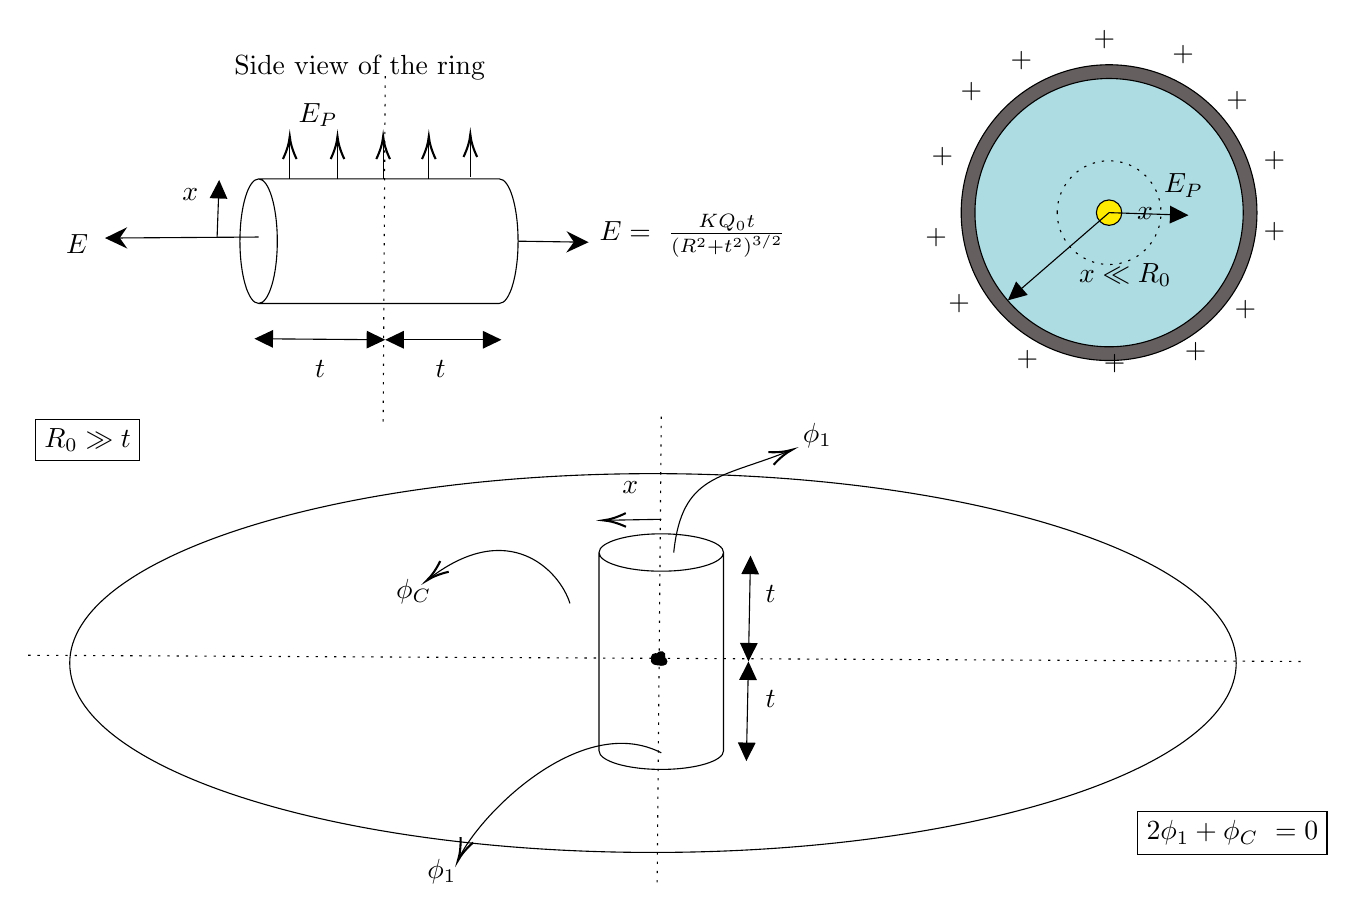
\begin{tikzpicture}[x=0.75pt,y=0.75pt,yscale=-1,xscale=1]
%uncomment if require: \path (0,446); %set diagram left start at 0, and has height of 446

%Shape: Can [id:dp15819190824810292] 
\draw   (137,89) -- (253,89) .. controls (257.97,89) and (262,102.43) .. (262,119) .. controls (262,135.57) and (257.97,149) .. (253,149) -- (137,149) .. controls (132.03,149) and (128,135.57) .. (128,119) .. controls (128,102.43) and (132.03,89) .. (137,89) .. controls (141.97,89) and (146,102.43) .. (146,119) .. controls (146,135.57) and (141.97,149) .. (137,149) ;
%Straight Lines [id:da41068477221279265] 
\draw    (137,117) -- (66,117.48) ;
\draw [shift={(63,117.5)}, rotate = 359.61] [fill={rgb, 255:red, 0; green, 0; blue, 0 }  ][line width=0.08]  [draw opacity=0] (10.72,-5.15) -- (0,0) -- (10.72,5.15) -- (7.12,0) -- cycle    ;
%Straight Lines [id:da8442222987689461] 
\draw    (117,117) -- (117.89,92.5) ;
\draw [shift={(118,89.5)}, rotate = 452.08] [fill={rgb, 255:red, 0; green, 0; blue, 0 }  ][line width=0.08]  [draw opacity=0] (8.93,-4.29) -- (0,0) -- (8.93,4.29) -- cycle    ;
%Straight Lines [id:da2625247075245154] 
\draw    (138,166.02) -- (195,166.48) ;
\draw [shift={(198,166.5)}, rotate = 180.45] [fill={rgb, 255:red, 0; green, 0; blue, 0 }  ][line width=0.08]  [draw opacity=0] (8.93,-4.29) -- (0,0) -- (8.93,4.29) -- cycle    ;
\draw [shift={(135,166)}, rotate = 0.45] [fill={rgb, 255:red, 0; green, 0; blue, 0 }  ][line width=0.08]  [draw opacity=0] (8.93,-4.29) -- (0,0) -- (8.93,4.29) -- cycle    ;
%Straight Lines [id:da4570297631367448] 
\draw    (201,166.5) -- (251,166.5) ;
\draw [shift={(254,166.5)}, rotate = 180] [fill={rgb, 255:red, 0; green, 0; blue, 0 }  ][line width=0.08]  [draw opacity=0] (8.93,-4.29) -- (0,0) -- (8.93,4.29) -- cycle    ;
\draw [shift={(198,166.5)}, rotate = 0] [fill={rgb, 255:red, 0; green, 0; blue, 0 }  ][line width=0.08]  [draw opacity=0] (8.93,-4.29) -- (0,0) -- (8.93,4.29) -- cycle    ;
%Straight Lines [id:da5310655891901901] 
\draw    (262,119) -- (293,119.46) ;
\draw [shift={(296,119.5)}, rotate = 180.84] [fill={rgb, 255:red, 0; green, 0; blue, 0 }  ][line width=0.08]  [draw opacity=0] (10.72,-5.15) -- (0,0) -- (10.72,5.15) -- (7.12,0) -- cycle    ;
%Straight Lines [id:da8928088652550399] 
\draw    (152,89) -- (152,70.5) ;
\draw [shift={(152,68.5)}, rotate = 450] [color={rgb, 255:red, 0; green, 0; blue, 0 }  ][line width=0.75]    (10.93,-3.29) .. controls (6.95,-1.4) and (3.31,-0.3) .. (0,0) .. controls (3.31,0.3) and (6.95,1.4) .. (10.93,3.29)   ;
%Straight Lines [id:da42724784975898533] 
\draw    (175,89) -- (175,70.5) ;
\draw [shift={(175,68.5)}, rotate = 450] [color={rgb, 255:red, 0; green, 0; blue, 0 }  ][line width=0.75]    (10.93,-3.29) .. controls (6.95,-1.4) and (3.31,-0.3) .. (0,0) .. controls (3.31,0.3) and (6.95,1.4) .. (10.93,3.29)   ;
%Straight Lines [id:da5269836097028531] 
\draw    (197,89) -- (197,70.5) ;
\draw [shift={(197,68.5)}, rotate = 450] [color={rgb, 255:red, 0; green, 0; blue, 0 }  ][line width=0.75]    (10.93,-3.29) .. controls (6.95,-1.4) and (3.31,-0.3) .. (0,0) .. controls (3.31,0.3) and (6.95,1.4) .. (10.93,3.29)   ;
%Straight Lines [id:da5147929730715581] 
\draw    (219,89) -- (219,70.5) ;
\draw [shift={(219,68.5)}, rotate = 450] [color={rgb, 255:red, 0; green, 0; blue, 0 }  ][line width=0.75]    (10.93,-3.29) .. controls (6.95,-1.4) and (3.31,-0.3) .. (0,0) .. controls (3.31,0.3) and (6.95,1.4) .. (10.93,3.29)   ;
%Straight Lines [id:da5389855025528796] 
\draw    (239,88) -- (239,69.5) ;
\draw [shift={(239,67.5)}, rotate = 450] [color={rgb, 255:red, 0; green, 0; blue, 0 }  ][line width=0.75]    (10.93,-3.29) .. controls (6.95,-1.4) and (3.31,-0.3) .. (0,0) .. controls (3.31,0.3) and (6.95,1.4) .. (10.93,3.29)   ;
%Straight Lines [id:da9726782656027295] 
\draw  [dash pattern={on 0.84pt off 2.51pt}]  (198,39.5) -- (197,206.5) ;
%Shape: Circle [id:dp9619821012071179] 
\draw  [fill={rgb, 255:red, 101; green, 95; blue, 95 }  ,fill opacity=1 ] (475.5,105.25) .. controls (475.5,65.9) and (507.4,34) .. (546.75,34) .. controls (586.1,34) and (618,65.9) .. (618,105.25) .. controls (618,144.6) and (586.1,176.5) .. (546.75,176.5) .. controls (507.4,176.5) and (475.5,144.6) .. (475.5,105.25) -- cycle ;
%Shape: Circle [id:dp732948933951294] 
\draw  [color={rgb, 255:red, 0; green, 0; blue, 0 }  ,draw opacity=1 ][fill={rgb, 255:red, 174; green, 220; blue, 227 }  ,fill opacity=1 ] (482.13,105.25) .. controls (482.13,69.56) and (511.06,40.63) .. (546.75,40.63) .. controls (582.44,40.63) and (611.38,69.56) .. (611.38,105.25) .. controls (611.38,140.94) and (582.44,169.88) .. (546.75,169.88) .. controls (511.06,169.88) and (482.13,140.94) .. (482.13,105.25) -- cycle ;
%Shape: Circle [id:dp8352910190885805] 
\draw  [fill={rgb, 255:red, 255; green, 235; blue, 0 }  ,fill opacity=1 ] (540.63,105.25) .. controls (540.63,101.87) and (543.37,99.13) .. (546.75,99.13) .. controls (550.13,99.13) and (552.88,101.87) .. (552.88,105.25) .. controls (552.88,108.63) and (550.13,111.38) .. (546.75,111.38) .. controls (543.37,111.38) and (540.63,108.63) .. (540.63,105.25) -- cycle ;
%Shape: Circle [id:dp8730299060620863] 
\draw  [dash pattern={on 0.84pt off 2.51pt}] (521.75,105.25) .. controls (521.75,91.44) and (532.94,80.25) .. (546.75,80.25) .. controls (560.56,80.25) and (571.75,91.44) .. (571.75,105.25) .. controls (571.75,119.06) and (560.56,130.25) .. (546.75,130.25) .. controls (532.94,130.25) and (521.75,119.06) .. (521.75,105.25) -- cycle ;
%Straight Lines [id:da1722254295607648] 
\draw    (546.75,105.25) -- (582,106.4) ;
\draw [shift={(585,106.5)}, rotate = 181.87] [fill={rgb, 255:red, 0; green, 0; blue, 0 }  ][line width=0.08]  [draw opacity=0] (8.93,-4.29) -- (0,0) -- (8.93,4.29) -- cycle    ;
%Straight Lines [id:da5064361980480354] 
\draw    (546.75,105.25) -- (500.27,145.54) ;
\draw [shift={(498,147.5)}, rotate = 319.09000000000003] [fill={rgb, 255:red, 0; green, 0; blue, 0 }  ][line width=0.08]  [draw opacity=0] (8.93,-4.29) -- (0,0) -- (8.93,4.29) -- cycle    ;
%Shape: Ellipse [id:dp6550766149413016] 
\draw   (46,322.25) .. controls (46,271.85) and (171.81,231) .. (327,231) .. controls (482.19,231) and (608,271.85) .. (608,322.25) .. controls (608,372.65) and (482.19,413.5) .. (327,413.5) .. controls (171.81,413.5) and (46,372.65) .. (46,322.25) -- cycle ;
%Shape: Can [id:dp0780646959371114] 
\draw   (361,269) -- (361,364.5) .. controls (361,369.47) and (347.57,373.5) .. (331,373.5) .. controls (314.43,373.5) and (301,369.47) .. (301,364.5) -- (301,269) .. controls (301,264.03) and (314.43,260) .. (331,260) .. controls (347.57,260) and (361,264.03) .. (361,269) .. controls (361,273.97) and (347.57,278) .. (331,278) .. controls (314.43,278) and (301,273.97) .. (301,269) ;
%Straight Lines [id:da5088975071595334] 
\draw  [dash pattern={on 0.84pt off 2.51pt}]  (331,203.5) -- (329,430.5) ;
%Straight Lines [id:da8520935926585673] 
\draw  [dash pattern={on 0.84pt off 2.51pt}]  (26,318.5) -- (641,321.5) ;
%Curve Lines [id:da375617962335254] 
\draw    (287,293.5) .. controls (282.05,277.66) and (257.5,252.02) .. (219.17,281.59) ;
\draw [shift={(218,282.5)}, rotate = 321.52] [color={rgb, 255:red, 0; green, 0; blue, 0 }  ][line width=0.75]    (10.93,-3.29) .. controls (6.95,-1.4) and (3.31,-0.3) .. (0,0) .. controls (3.31,0.3) and (6.95,1.4) .. (10.93,3.29)   ;
%Shape: Free Drawing [id:dp9039256585878004] 
\draw  [color={rgb, 255:red, 0; green, 0; blue, 0 }  ][line width=3] [line join = round][line cap = round] (331,318.5) .. controls (330.53,318.5) and (330,319.03) .. (330,319.5) ;
%Shape: Free Drawing [id:dp5738520344960787] 
\draw  [color={rgb, 255:red, 0; green, 0; blue, 0 }  ][line width=3] [line join = round][line cap = round] (328,319.5) .. controls (331.67,319.5) and (331,321.5) .. (331,321.5) .. controls (331,321.5) and (331,320.17) .. (331,319.5) ;
%Shape: Free Drawing [id:dp2196446468549671] 
\draw  [color={rgb, 255:red, 0; green, 0; blue, 0 }  ][line width=3] [line join = round][line cap = round] (331,320.5) .. controls (326.13,320.5) and (327.53,321.5) .. (332,321.5) ;
%Curve Lines [id:da906931331490308] 
\draw    (337,269) .. controls (340.94,231.08) and (359.43,233.42) .. (392.48,220.12) ;
\draw [shift={(394,219.5)}, rotate = 517.62] [color={rgb, 255:red, 0; green, 0; blue, 0 }  ][line width=0.75]    (10.93,-3.29) .. controls (6.95,-1.4) and (3.31,-0.3) .. (0,0) .. controls (3.31,0.3) and (6.95,1.4) .. (10.93,3.29)   ;
%Straight Lines [id:da5243188936789058] 
\draw    (373.06,318.5) -- (373.94,273.5) ;
\draw [shift={(374,270.5)}, rotate = 451.12] [fill={rgb, 255:red, 0; green, 0; blue, 0 }  ][line width=0.08]  [draw opacity=0] (8.93,-4.29) -- (0,0) -- (8.93,4.29) -- cycle    ;
\draw [shift={(373,321.5)}, rotate = 271.12] [fill={rgb, 255:red, 0; green, 0; blue, 0 }  ][line width=0.08]  [draw opacity=0] (8.93,-4.29) -- (0,0) -- (8.93,4.29) -- cycle    ;
%Straight Lines [id:da6438530767576001] 
\draw    (372.06,366.5) -- (372.94,324.5) ;
\draw [shift={(373,321.5)}, rotate = 451.19] [fill={rgb, 255:red, 0; green, 0; blue, 0 }  ][line width=0.08]  [draw opacity=0] (8.93,-4.29) -- (0,0) -- (8.93,4.29) -- cycle    ;
\draw [shift={(372,369.5)}, rotate = 271.19] [fill={rgb, 255:red, 0; green, 0; blue, 0 }  ][line width=0.08]  [draw opacity=0] (8.93,-4.29) -- (0,0) -- (8.93,4.29) -- cycle    ;
%Straight Lines [id:da11745459041895345] 
\draw    (331,253) -- (305,253.46) ;
\draw [shift={(303,253.5)}, rotate = 358.98] [color={rgb, 255:red, 0; green, 0; blue, 0 }  ][line width=0.75]    (10.93,-3.29) .. controls (6.95,-1.4) and (3.31,-0.3) .. (0,0) .. controls (3.31,0.3) and (6.95,1.4) .. (10.93,3.29)   ;
%Curve Lines [id:da637879725329126] 
\draw    (331,365.5) .. controls (292.97,346) and (244.49,393.99) .. (233.75,415.87) ;
\draw [shift={(233,417.5)}, rotate = 293.2] [color={rgb, 255:red, 0; green, 0; blue, 0 }  ][line width=0.75]    (10.93,-3.29) .. controls (6.95,-1.4) and (3.31,-0.3) .. (0,0) .. controls (3.31,0.3) and (6.95,1.4) .. (10.93,3.29)   ;

% Text Node
\draw (124,28) node [anchor=north west][inner sep=0.75pt]   [align=left] {Side view of the ring};
% Text Node
\draw (43,114.4) node [anchor=north west][inner sep=0.75pt]    {$E$};
% Text Node
\draw (99,92.4) node [anchor=north west][inner sep=0.75pt]    {$x$};
% Text Node
\draw (163,175.4) node [anchor=north west][inner sep=0.75pt]    {$t$};
% Text Node
\draw (221,175.4) node [anchor=north west][inner sep=0.75pt]    {$t$};
% Text Node
\draw (155,51.4) node [anchor=north west][inner sep=0.75pt]    {$E_{P}$};
% Text Node
\draw (300,104.9) node [anchor=north west][inner sep=0.75pt]    {$E=\ \frac{KQ_{0} t}{\left( R^{2} +t^{2}\right)^{3/2}}$};
% Text Node
\draw (538,16.4) node [anchor=north west][inner sep=0.75pt]    {$+$};
% Text Node
\draw (576,23.4) node [anchor=north west][inner sep=0.75pt]    {$+$};
% Text Node
\draw (602,45.4) node [anchor=north west][inner sep=0.75pt]    {$+$};
% Text Node
\draw (620,74.4) node [anchor=north west][inner sep=0.75pt]    {$+$};
% Text Node
\draw (620,108.65) node [anchor=north west][inner sep=0.75pt]    {$+$};
% Text Node
\draw (606,146.4) node [anchor=north west][inner sep=0.75pt]    {$+$};
% Text Node
\draw (582,166.4) node [anchor=north west][inner sep=0.75pt]    {$+$};
% Text Node
\draw (543,172.4) node [anchor=north west][inner sep=0.75pt]    {$+$};
% Text Node
\draw (501,170.4) node [anchor=north west][inner sep=0.75pt]    {$+$};
% Text Node
\draw (468,143.4) node [anchor=north west][inner sep=0.75pt]    {$+$};
% Text Node
\draw (457,111.4) node [anchor=north west][inner sep=0.75pt]    {$+$};
% Text Node
\draw (460,72.4) node [anchor=north west][inner sep=0.75pt]    {$+$};
% Text Node
\draw (474,41.4) node [anchor=north west][inner sep=0.75pt]    {$+$};
% Text Node
\draw (498,26.4) node [anchor=north west][inner sep=0.75pt]    {$+$};
% Text Node
\draw (572,85.4) node [anchor=north west][inner sep=0.75pt]    {$E_{P}$};
% Text Node
\draw (559,101.4) node [anchor=north west][inner sep=0.75pt]    {$x$};
% Text Node
\draw (531,128.4) node [anchor=north west][inner sep=0.75pt]    {$x\ll R_{0}$};
% Text Node
\draw (202,280.4) node [anchor=north west][inner sep=0.75pt]    {$\phi _{C}$};
% Text Node
\draw (398,205.4) node [anchor=north west][inner sep=0.75pt]    {$\phi _{1}$};
% Text Node
\draw (380,283.4) node [anchor=north west][inner sep=0.75pt]    {$t$};
% Text Node
\draw (380,334.4) node [anchor=north west][inner sep=0.75pt]    {$t$};
% Text Node
\draw (311,233.4) node [anchor=north west][inner sep=0.75pt]    {$x$};
% Text Node
\draw (217,415.4) node [anchor=north west][inner sep=0.75pt]    {$\phi _{1}$};
% Text Node
\draw (559,392.4) node [anchor=north west][inner sep=0.75pt]    {\fbox{$2\phi _{1} +\phi _{C} \ =0$}};
% Text Node
\draw (28,203.4) node [anchor=north west][inner sep=0.75pt]    {\fbox{$R_{0} \gg t$}};

\end{tikzpicture}
\end{center}
$$2\cdot E\cdot\pi x^2 + E_P\cdot 2\pi x\cdot2t=0$$ \\
$$E_P=-\frac{E\cdot x}{2t}=\frac{KQ_0t}{(R^2+t^2)^{3/2}}\cdot\frac{x}{2t}$$ \\
$$E_P=\frac{KQ_0x}{2R^3}$$
Direction towards the center of the ring.

{\Large{\textbf{Calculation of Magnetic Field:}}}
$$I=\frac{QW}{2\pi}$$ \\
%insert image 
\begin{center}
    
 
\tikzset{every picture/.style={line width=0.75pt}} %set default line width to 0.75pt        

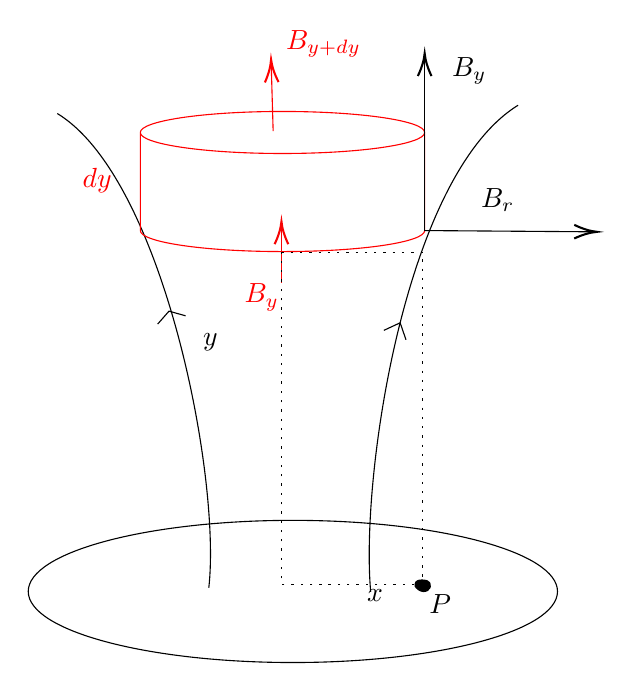
\begin{tikzpicture}[x=0.75pt,y=0.75pt,yscale=-1,xscale=1]
%uncomment if require: \path (0,398); %set diagram left start at 0, and has height of 398

%Shape: Ellipse [id:dp2804663484043828] 
\draw   (225,315.75) .. controls (225,296.83) and (282.08,281.5) .. (352.5,281.5) .. controls (422.92,281.5) and (480,296.83) .. (480,315.75) .. controls (480,334.67) and (422.92,350) .. (352.5,350) .. controls (282.08,350) and (225,334.67) .. (225,315.75) -- cycle ;
%Curve Lines [id:da1187754695910288] 
\draw    (390,316) .. controls (385,261.5) and (406,115.5) .. (461,81.5) ;
%Curve Lines [id:da29711424557538346] 
\draw    (312,314) .. controls (318,260.5) and (290,116.5) .. (239,85.5) ;
%Shape: Can [id:dp3047546383899997] 
\draw  [color={rgb, 255:red, 255; green, 0; blue, 0 }  ,draw opacity=1 ] (416,94.63) -- (416,141.88) .. controls (416,147.47) and (385.33,152) .. (347.5,152) .. controls (309.67,152) and (279,147.47) .. (279,141.88) -- (279,94.63) .. controls (279,89.03) and (309.67,84.5) .. (347.5,84.5) .. controls (385.33,84.5) and (416,89.03) .. (416,94.63) .. controls (416,100.22) and (385.33,104.75) .. (347.5,104.75) .. controls (309.67,104.75) and (279,100.22) .. (279,94.63) ;
%Straight Lines [id:da9705152159035346] 
\draw [color={rgb, 255:red, 255; green, 0; blue, 0 }  ,draw opacity=1 ]   (343,94) -- (342.06,61.5) ;
\draw [shift={(342,59.5)}, rotate = 448.34] [color={rgb, 255:red, 255; green, 0; blue, 0 }  ,draw opacity=1 ][line width=0.75]    (10.93,-3.29) .. controls (6.95,-1.4) and (3.31,-0.3) .. (0,0) .. controls (3.31,0.3) and (6.95,1.4) .. (10.93,3.29)   ;
%Straight Lines [id:da4447897859433789] 
\draw [color={rgb, 255:red, 246; green, 4; blue, 4 }  ,draw opacity=1 ]   (347,167) -- (347,139.5) ;
\draw [shift={(347,137.5)}, rotate = 450] [color={rgb, 255:red, 246; green, 4; blue, 4 }  ,draw opacity=1 ][line width=0.75]    (10.93,-3.29) .. controls (6.95,-1.4) and (3.31,-0.3) .. (0,0) .. controls (3.31,0.3) and (6.95,1.4) .. (10.93,3.29)   ;
\draw   (287.36,186.95) -- (292.82,180.71) -- (300.8,182.95) ;
\draw   (396.35,189.96) -- (404.19,186.32) -- (407,194.5) ;
%Shape: Rectangle [id:dp2677073987245866] 
\draw  [dash pattern={on 0.84pt off 2.51pt}] (347,152.25) -- (415,152.25) -- (415,312.5) -- (347,312.5) -- cycle ;
%Straight Lines [id:da9281588105501917] 
\draw    (416,141.88) -- (416,58.5) ;
\draw [shift={(416,56.5)}, rotate = 450] [color={rgb, 255:red, 0; green, 0; blue, 0 }  ][line width=0.75]    (10.93,-3.29) .. controls (6.95,-1.4) and (3.31,-0.3) .. (0,0) .. controls (3.31,0.3) and (6.95,1.4) .. (10.93,3.29)   ;
%Straight Lines [id:da6460517338951173] 
\draw    (416,141.88) -- (497,142.48) ;
\draw [shift={(499,142.5)}, rotate = 180.43] [color={rgb, 255:red, 0; green, 0; blue, 0 }  ][line width=0.75]    (10.93,-3.29) .. controls (6.95,-1.4) and (3.31,-0.3) .. (0,0) .. controls (3.31,0.3) and (6.95,1.4) .. (10.93,3.29)   ;
%Shape: Free Drawing [id:dp33977752710877707] 
\draw  [color={rgb, 255:red, 0; green, 0; blue, 0 }  ][line width=3] [line join = round][line cap = round] (416,312.5) .. controls (420.01,312.5) and (409.96,310.81) .. (414,313.5) .. controls (416.63,315.25) and (418.32,312.5) .. (416,312.5) -- cycle ;

% Text Node
\draw (348,44.4) node [anchor=north west][inner sep=0.75pt]  [color={rgb, 255:red, 255; green, 0; blue, 0 }  ,opacity=1 ]  {$B_{y+dy}$};
% Text Node
\draw (250,110.4) node [anchor=north west][inner sep=0.75pt]  [color={rgb, 255:red, 255; green, 0; blue, 0 }  ,opacity=1 ]  {$dy$};
% Text Node
\draw (328,166.4) node [anchor=north west][inner sep=0.75pt]  [color={rgb, 255:red, 255; green, 0; blue, 0 }  ,opacity=1 ]  {$B_y$};
% Text Node
\draw (428,57.4) node [anchor=north west][inner sep=0.75pt]    {$B_{y}$};
% Text Node
\draw (442,120.4) node [anchor=north west][inner sep=0.75pt]    {$B_{r}$};
% Text Node
\draw (387,313.4) node [anchor=north west][inner sep=0.75pt]    {$x$};
% Text Node
\draw (417,315.9) node [anchor=north west][inner sep=0.75pt]    {$P$};
% Text Node
\draw (308,190.4) node [anchor=north west][inner sep=0.75pt]    {$y$};


\end{tikzpicture}
\end{center}
$$B_y|_{axis}=\frac{\mu_0IR^2}{2(R^2+y^2)^{3/2}}$$
Near the axis :- $x\ll R$ 

{\Large{\textbf{{\underline{To find $B_r$:}}}}}
Using Gauss Theorem
\begin{center}
    $$B_{y+dy}\cdot\pi x^2 - B_y\cdot\pi x^2 + B_r\cdot2\pi x\cdot dy=0$$ \\
    $$B_r=\frac{-x}{2}(\frac{B_{y+dy}-B_y}{dy})=\frac{-x}{2}\cdot\frac{dB}{dy}$$ \\
    $$B_r=\frac{-x}{2}\cdot\frac{\mu_0IR^2}{2}\cdot\frac{d}{dy}[R^2+y^2]^{-3/2}$$
    $$B_r=-\frac{\mu_0IR^2x}{4}\cdot\frac{-3}{2}\cdot2y\cdot[R^2+y^2]^{-5/2}$$
    $$B_r=\frac{3\mu_0IR^2xy}{4(R^2+y^2)^{5/3}}$$
\end{center}
\color{black} $h\rightarrow 0$ 
\color{black} $\Rightarrow$
\color{black} Point $A$ and $B$ are very close to axis \\
\color{black} $$B_0=\frac{\mu_0I}{2R}$$
\color{black} 

%insert image
\begin{center}
    
\tikzset{every picture/.style={line width=0.75pt}} %set default line width to 0.75pt        

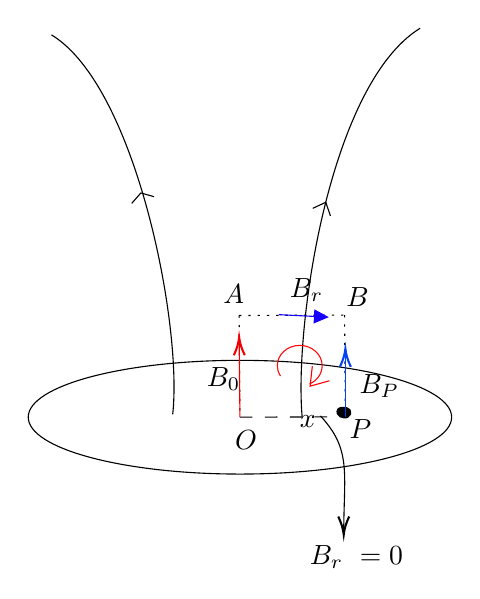
\begin{tikzpicture}[x=0.60pt,y=0.60pt,yscale=-1,xscale=1]
%uncomment if require: \path (0,398); %set diagram left start at 0, and has height of 398

%Shape: Ellipse [id:dp2804663484043828] 
\draw   (221,258.75) .. controls (221,239.83) and (278.08,224.5) .. (348.5,224.5) .. controls (418.92,224.5) and (476,239.83) .. (476,258.75) .. controls (476,277.67) and (418.92,293) .. (348.5,293) .. controls (278.08,293) and (221,277.67) .. (221,258.75) -- cycle ;
%Curve Lines [id:da1187754695910288] 
\draw    (386,259) .. controls (381,204.5) and (402,58.5) .. (457,24.5) ;
%Curve Lines [id:da29711424557538346] 
\draw    (308,257) .. controls (314,203.5) and (286,59.5) .. (235,28.5) ;
\draw   (283.36,129.95) -- (288.82,123.71) -- (296.8,125.95) ;
\draw   (392.35,132.96) -- (400.19,129.32) -- (403,137.5) ;
%Shape: Free Drawing [id:dp33977752710877707] 
\draw  [color={rgb, 255:red, 0; green, 0; blue, 0 }  ][line width=3] [line join = round][line cap = round] (412,255.5) .. controls (416.01,255.5) and (405.96,253.81) .. (410,256.5) .. controls (412.63,258.25) and (414.32,255.5) .. (412,255.5) -- cycle ;
%Straight Lines [id:da7750462412023267] 
\draw  [dash pattern={on 4.5pt off 4.5pt}]  (348.5,258.75) -- (412,258.5) ;
%Straight Lines [id:da5092487360415987] 
\draw  [dash pattern={on 0.84pt off 2.51pt}]  (348,197.5) -- (348.5,258.75) ;
%Straight Lines [id:da5012765009963169] 
\draw  [dash pattern={on 0.84pt off 2.51pt}]  (411.5,197.25) -- (412,258.5) ;
%Straight Lines [id:da13366551569980412] 
\draw  [dash pattern={on 0.84pt off 2.51pt}]  (348,197.5) -- (411.5,197.25) ;
%Straight Lines [id:da23220113707244616] 
\draw [color={rgb, 255:red, 21; green, 0; blue, 255 }  ,draw opacity=1 ]   (372,197) -- (399,198.35) ;
\draw [shift={(402,198.5)}, rotate = 182.86] [fill={rgb, 255:red, 21; green, 0; blue, 255 }  ,fill opacity=1 ][line width=0.08]  [draw opacity=0] (8.93,-4.29) -- (0,0) -- (8.93,4.29) -- cycle    ;
%Straight Lines [id:da9194837872069539] 
\draw [color={rgb, 255:red, 244; green, 0; blue, 0 }  ,draw opacity=1 ]   (348.5,258.75) -- (348.02,212.5) ;
\draw [shift={(348,210.5)}, rotate = 449.41] [color={rgb, 255:red, 244; green, 0; blue, 0 }  ,draw opacity=1 ][line width=0.75]    (10.93,-3.29) .. controls (6.95,-1.4) and (3.31,-0.3) .. (0,0) .. controls (3.31,0.3) and (6.95,1.4) .. (10.93,3.29)   ;
%Straight Lines [id:da9730008787541697] 
\draw [color={rgb, 255:red, 4; green, 66; blue, 239 }  ,draw opacity=1 ]   (412,258.5) -- (412,219.5) ;
\draw [shift={(412,217.5)}, rotate = 450] [color={rgb, 255:red, 4; green, 66; blue, 239 }  ,draw opacity=1 ][line width=0.75]    (10.93,-3.29) .. controls (6.95,-1.4) and (3.31,-0.3) .. (0,0) .. controls (3.31,0.3) and (6.95,1.4) .. (10.93,3.29)   ;
%Curve Lines [id:da8349556629731556] 
\draw    (397,258) .. controls (415.72,278.19) and (411.14,292.08) .. (411,327.85) ;
\draw [shift={(411,329.5)}, rotate = 270] [color={rgb, 255:red, 0; green, 0; blue, 0 }  ][line width=0.75]    (10.93,-3.29) .. controls (6.95,-1.4) and (3.31,-0.3) .. (0,0) .. controls (3.31,0.3) and (6.95,1.4) .. (10.93,3.29)   ;
%Shape: Arc [id:dp5014699045879913] 
\draw  [draw opacity=0] (372.87,233.97) .. controls (371.68,232.14) and (371,230.02) .. (371,227.75) .. controls (371,220.98) and (377.04,215.5) .. (384.5,215.5) .. controls (391.96,215.5) and (398,220.98) .. (398,227.75) .. controls (398,232.58) and (394.92,236.76) .. (390.44,238.75) -- (384.5,227.75) -- cycle ; \draw  [color={rgb, 255:red, 255; green, 11; blue, 11 }  ,draw opacity=1 ] (372.87,233.97) .. controls (371.68,232.14) and (371,230.02) .. (371,227.75) .. controls (371,220.98) and (377.04,215.5) .. (384.5,215.5) .. controls (391.96,215.5) and (398,220.98) .. (398,227.75) .. controls (398,232.58) and (394.92,236.76) .. (390.44,238.75) ;
\draw  [color={rgb, 255:red, 255; green, 0; blue, 0 }  ,draw opacity=1 ] (402.38,236.81) -- (390.76,240.06) -- (392.09,228.07) ;

% Text Node
\draw (383,256.4) node [anchor=north west][inner sep=0.75pt]    {$x$};
% Text Node
\draw (413,258.9) node [anchor=north west][inner sep=0.75pt]    {$P$};
% Text Node
\draw (377,173.4) node [anchor=north west][inner sep=0.75pt]    {$B_{r}$};
% Text Node
\draw (337,177.4) node [anchor=north west][inner sep=0.75pt]    {$A$};
% Text Node
\draw (411,179.4) node [anchor=north west][inner sep=0.75pt]    {$B$};
% Text Node
\draw (344,265.4) node [anchor=north west][inner sep=0.75pt]    {$O$};
% Text Node
\draw (327,227.4) node [anchor=north west][inner sep=0.75pt]    {$B_{0}$};
% Text Node
\draw (419,231.4) node [anchor=north west][inner sep=0.75pt]    {$B_{P}$};
% Text Node
\draw (389,334.4) node [anchor=north west][inner sep=0.75pt]    {$B_{r} \ =0$};


\end{tikzpicture} 
\end{center}


Using Amperes Law :
\begin{center}
    $$\underbrace{\int_{0}^{A}\vec{B}\cdot\vec{dl}}_{+B_0h}+\int_{A}^{B}\vec{B_r}\cdot\vec{dl}+\underbrace{\int_{\textbf{B}}^{P}\vec{B_p}\cdot\vec{dl}}_{-B_ph}+\underbrace{\int_{0}^{P}\vec{B}\cdot\vec{dl}}_{0}=0$$ \\
    $$\int_{A}^{B}\vec{B_r}\cdot\vec{dl}=\int_{0}^{x}\frac{3\mu_0IR^2xh}{4(R^2+y^2)^{5/3}}\cdot dx=\frac{3\mu_0IR^2x^2h}{8(R^2+y^2)^{5/3}}=\frac{3\mu_0IR^2x^2h}{8R^5}=\frac{3\mu_0Ix^2h}{8R^3}$$
\end{center}
\flushright
\fbox{$R \gg h$} \\

\flushleft
$$\Rightarrow +B_0h - B_ph +\frac{3\mu_0Ix^2h}{8R^3}=0$$
$$B_p=B_0+\frac{3\mu_0Ix^2}{8R^3}$$
$$B_p=\frac{\mu_0I}{2R}[1+\frac{3x^2}{4R^2}]$$
$$B_p=\frac{\mu_0}{2R}\cdot\frac{QW}{2\pi}(1+\frac{3x^2}{4R^2})=\frac{\mu_0QW}{4\pi R}(1+\frac{3x^2}{4R^2})$$

$$E_p=\frac{kQ_0x}{2R^3}=\frac{1}{4\pi\epsilon_0}\cdot\frac{Q_0x}{2R^3}=\frac{Q_0x}{8\pi\epsilon_0R^3}$$
$$\frac{E_p}{B_p}=\frac{2x^2}{w[4R^2+3x^2]}$$ \\


\end{solution}



%Aditya's solution
%\begin{solution}
%focal length $(f)$ of this lens :- $$ f^{-1} = %\frac{R}{n-1}$$ According to geometry :- $n$sin$\alpha$ = %sin$(\alpha +\beta)$ and $$\alpha = sin^{-1} \frac{h}{R}$$ %& $$ \alpha + \beta = sin^{-1} \frac{nh}{R} $$ %Distance$(l)$ :- $l$ = $h$ cot $\beta$ = $h$ cot %$(sin^{-1} %(\frac{nh}{R} - sin^{-1} \frac{h}{R}))$ %$$\delta x = R - %\sqrt(R^2 - h^2) $$ and we can write %$\delta{s '} = l - %\delta x - f' $ writing all the value, %we get:- $$ %\delta{s'} = \frac{\sqrt{R^2 - n^2 h^2} %\sqrt{R^2 -h^2} + n %h^2}{n \sqrt{R^2 - n^2} - \sqrt{R^2 - %n h^2}} %-\frac{nR}{n-1} + \sqrt{R^2 - h^2} $$ $$= \frac{n %\sqrt{R^2 %-n^2 h^2} + \sqrt{R^2 - h^2}}{n^2 -1 } - \frac{ %nR}{n-1} + %\sqrt{R^2 -h^2} $$ We get, $ \delta s' = %\frac{-h^2 %n^2}{2R(n-1)}$\\

%and from similarity of the triangle, we get $$\frac{h}{f}= %\frac{\delta g'}{\mid \delta s' \mid}$$\\
%$\therefore \delta g' = \mid \delta s' \mid \frac{h}{f} = %\frac{h^3 n^2}{R^2} $
%\end{solution}






\end{document}